% -----------------------------------------------------------------------------------
% This template is brought to you by the Laboratory for                             %
% Electrical Instrumentation and Embedded Systems                                   %
% at the Albert-Ludwigs-Universität in Freiburg                                     %
%                                                                                   %
% Please note: We do not provide technical support for this template                %
% However, please feel free to contribute to this template on GitHub                %
% https://github.com/imtekalex/emes_template                                        %
%                                                                                   %
% Special thanks go out to                                                          %
% Till Steinmann and Andreas Reichenbach                                            %
% -----------------------------------------------------------------------------------

% ToDo:
% Centralize Language settings so that individual chapters are also built correctly.
% Speed up build process

% Document settings
\input{settings+/docclass}
% WARNING: Proceed with caution!

% -----------------------------------------------------------------------------------
% For package standalone
% -----------------------------------------------------------------------------------
\usepackage{import}

% -----------------------------------------------------------------------------------
% Language and typeset
% -----------------------------------------------------------------------------------
\usepackage[ngerman, english]{babel}

\usepackage{subcaption}
% Umlauts and other special characters (UTF-8)
% \usepackage[utf8]{inputenc}
\usepackage{fontspec}
\setsansfont{Arial}
% \usepackage[T1]{fontenc}  % Enable accented characters and umlauts
% LuaLatex doesn't need fontenc and uses UTF-8
% \usepackage{lmodern}  % Font face


% --------------------------------------------------------------------------------
% Page formatting
% --------------------------------------------------------------------------------
% Change the header/footer for chapter beginnings and normal pages
\usepackage[automark,headsepline]{scrlayer-scrpage}

% The package provides an easy and flexible user interface to customize the page
% layout, implementing auto-centering and auto-balancing mechanisms
% WARNING: WHEN CHANGING BCOR (Binding correction), the cover needs reworking!...
\newcommand{\theBCOR}{15mm}  % Define binding correction
\usepackage[
    bindingoffset=\theBCOR,
    % showframe, % Show boxes which indicate margins and paddings
    bottom = 3.5cm, % Margins
      left = 2.5cm,
     right = 2.5cm
] {geometry}

% The package 'float' provides a container for document objects which can not be
% broken over pages, such as tables and figures
% Needed for table and figure indexes  
\usepackage{float}

% support for landscape layout
\usepackage{lscape}

% support of \tablenotes command to add notes under table
\usepackage{threeparttable}

% To allow drawing more professional tables
\usepackage{booktabs}

% --------------------------------------------------------------------------------
% Contents
% --------------------------------------------------------------------------------
% Vector graphics (for Cover page)
\usepackage{tikz} 

% Allows additional parameters when including images
\usepackage{graphicx}

% Roman font family for all headings
\addtokomafont{disposition}{\rmfamily}

% Set the line spacing to 1.5
\usepackage[onehalfspacing]{setspace}

% Improves overall text spacing
% http://www.khirevich.com/latex/microtype/
\usepackage[stretch=10]{microtype}

% Math symbols like mu outside the math environment
\usepackage{textcomp}

% A comprehensive (SI) units package∗
% For defining SI units
\usepackage[
    range-units=single,         % Formatting ranges with single unit indication: 1 - 2 m
    range-phrase=-,             % Phrase for range: 1 - 2 m vs 1 to 2 m
    separate-uncertainty=true,  % sets +- between value and uncertainty 
    multi-part-units=repeat     % In expressions with multiple values (multi part numbers) 
                                % the unit is printed each time: 1 mm x 1 mm
] {siunitx}
% https://tex.stackexchange.com/questions/124488/multi-part-numbers-and-units-in-siunitx

% Allows Sourcecodes with highlighting 
\usepackage{listings}

% This package provides user control over the layout of the three basic list
% environments: enumerate, itemize and description
\usepackage{enumitem}
\setlist{nosep} % Remove the vertical space between \item elements in all lists

% ToDo Notes
% \setlength{\marginparwidth}{2cm}
\usepackage{todonotes}
\setuptodonotes{inline, inlinepar}
\reversemarginpar  % Put ToDo notes on the binding's side
% \usepackage{soul} % Colorful ToDo notes

% Check out colors here http://latexcolor.com/
\usepackage{xcolor}

\usepackage{amsmath}    % alignment of equations

% --------------------------------------------------------------------------------
% Other elements
% --------------------------------------------------------------------------------
% Blindtext: Organic looking text dummy
\usepackage{blindtext}

% Hyperlinks within the document (PDF)
% "hidelinks" hides visual highlighting of links
\usepackage[hidelinks]{hyperref}

% Package for Glossary and Index (Acronyms are listed in a separate list) 
\usepackage[acronym, nogroupskip]{glossaries}[=v4.49] % groupskip: alphabetic grouping of entries

\usepackage{xltabular}   % <------- FOR glossaries

% Integration and management of bibliographies
\usepackage{csquotes}   % backend=biber in biblatex needs this package
\usepackage[
    style=ieee,   % style of the bibliography, entries are sorted in alphabetic order. "ieee" is another common style.
    backend=biber,      % based on package 'biber' 
    bibencoding=ascii   % ASCII Text encoding; may use "utf8" instead
] {biblatex}

% --------------------------------------------------------------------------------
%                               PATHS & FILES
% --------------------------------------------------------------------------------
% Fix paths for standalone compiling
\ifstandalone
    \def \home {..}
\else
    \def \home {.}
\fi

% Package: scrlayer-scrpage
% \def \stylePath {\home/settings+/style/page}
\input{\home/settings+/style/page}  % Load page style

% Package: graphicx
\graphicspath{{\home/images/}}  % Set path to images

% Package: listings
\input{\home/settings+/style/code.tex}  % Set path to style file
\lstset{inputpath={\home/code/}} % Default path to code listings

% Package: glossaries
\input{\home/settings+/style/symbols}  % Set path to symbols list style file
\input{\home/settings+/style/acronyms}  % Set path to acronym list style file
% -------------------------------------------------------------------------------
%               Listing of all Glossary and Acronym Entries 
%                           use as shown below
% -------------------------------------------------------------------------------

% ==== EXEMPLARY ENTRY FOR SYMBOLS LIST =========================================

% ==== EXEMPLARY ENTRY FOR ACRONYMS LIST ========================================
% \newacronym{#label}{#acronym}{#long_form}

% define new command for custom arconym entry with only two arguments
% fabricates an easier way to use \newacronym 
\newcommand{\acroX}[2]{\newacronym{#1}{#1}{#2}}
% \acroX{label and arconym}{long name}
% \acroX{CD}               {Compact Disk}

\newcommand{\acroY}[3]{\newacronym{#1}{#2}{#3}}
% \arcoY{label}{acronym}{long name}
% \acroY{CD}   {cd}     {Compact Disk}
 
\newacronym{AEP}{AEP}{Imbalance price}
\newacronym{aFRR}{aFRR}{Automatic Frequency Restoration Reserve}


\newacronym{reBAP}{reBAP}{Uniform imbalance price}
\newacronym{TSO}{TSO}{Transmission System Operator}
\newacronym{FCR}{FCR}{Frequency Containment Reserve}
\newacronym{mFRR}{mFRR}{Manual Frequency Restoration Reserve}
\newacronym{BRP}{BRP}{Balancing Responsible Party}
\newacronym{SB}{SB}{System Balance}
\newacronym{VRE}{VRE}{variable renewable energy}
\newacronym{ID1}{ID1}{intraday index ID1}
\newacronym{MAE}{MAE}{mean average error}
\newacronym{RMSE}{RMSE}{root mean squared error}
\newacronym{MSE}{MSE}{mean squared error}
\newacronym{CRPS}{CRPS}{continuous ranked probabililty score}
\newacronym{GCC}{GCC}{Grid Control Cooperation}
\newacronym{IC}{IC}{Continuous intraday}
\newacronym{VWAP}{VWAP}{volume-weighted average price}
\newacronym{VID}{VID}{traded volume within the intraday market}
\newacronym{ID AEP}{ID AEP}{Intraday Average Energy Price}
\newacronym{FRR}{FRR}{Frequency Restoration Reserve}
\newacronym{TFT}{TFT}{Temporal Fusion Transformer}
\newacronym{DLM}{DLM}{Dynamic Linear Model}
\newacronym{GB}{GB}{Gradient Boosting}
\newacronym{RF}{RF}{Random Forest}
\newacronym{ARIMAX}{ARIMAX}{Autoregressive Integrated Moving Average with eXogenous variables}
\newacronym{xLSTM}{xLSTM}{Extended Long Short-Term Memory}
\newacronym{DWD}{DWD}{Deutscher Wetterdienst}
\newacronym{ENTSO-E}{ENTSO-E}{European Network of Transmission System Operators for Electricity}
\newacronym{IDA1}{IDA1}{Intraday auction 1}
\newacronym{MOSMIX}{MOSMIX}{Model Output Statistics-MIX}
\newacronym{mLSTM}{mLSTM}{memory-optimized LSTM}
\newacronym{sLSTM}{sLSTM}{speed-optimized LSTM}

% ==== EXEMPLARY ENTRY FOR MAIN GLOSSARY ========================================

    % \newglossaryentry{policy}{name={Policy},description={Im geschäftlichen Bereich bezeichnet Policy eine interne Leit- bzw. Richtlinie, die formal durch das Unternehmen dokumentiert und über ihr Management verantwortet wird}}
    % \newglossaryentry{pcie}{name={PCI Express},description={PCI Express („Peripheral Component Interconnect Express“, abgekürzt PCIe oder PCI-E) ist ein Standard zur Verbindung von Peripheriegeräten mit dem Chipsatz eines Hauptprozessors. PCIe ist der Nachfolger von PCI, PCI-X und AGP und bietet im Vergleich zu seinen Vorgängern eine höhere Datenübertragungsrate pro Pin.}}
    % \newglossaryentry{realnumber}
  % Load glossary, symbol and acronyms list

% Package: biblatex
\addbibresource{\home/references/references.bib}  % Set path to bib resources

% Custom variables
\input{\home/settings+/variables}
% --------------------------------------------------------------------------------
%                                   OPTIONAL
% --------------------------------------------------------------------------------


% Simple arithmetic for LaTeX commands
% \usepackage{calc}

% Document Elements
% -------------------

% Index
% \usepackage{imakeidx}

% compact Lists
%\usepackage{paralist}

% visual improvements for citations
% \usepackage{epigraph}

% Create pseudo code
% https://www.overleaf.com/learn/latex/Algorithms
% \usepackage{algorithm}
% \usepackage{algorithmic}
%\usepackage[noend]{algpseudocode}

% Formatting
% -------------------
% Tweaks for scrbook, redefines commands of other packages
% \usepackage{scrhack}

% Intelligent space separator (nice for superscript?)
% \usepackage{xspace}

% Allows breaks within tables
%\usepackage{tabularx}

% Allows for page breaks in tables
% \usepackage{longtable}

% allows modifying of captions
% \usepackage{caption}

% Multiline comments
%\usepackage{verbatim}

% % Custom colors
% \definecolor{dartmouthgreen}{rgb}{0.05, 0.5, 0.06}

% IF you want to define unicode characters
% \DeclareUnicodeCharacter{0229}{\c{e}}
% \DeclareUnicodeCharacter{0306}{\u{Z}}


% Document elements
% ------------------------------------

% Table package
% \usepackage{booktabs}

% Pie diagram
% \usepackage{datapie}

% Side by Side images
% \usepackage{subcaption}

% For landscape tables
%\usepackage{pdflscape}
%\usepackage{afterpage}

% Graphics can be flow around by text
%\usepackage{wrapfig}
  % Custom variables are located in settings+/variables.tex

% -----------------------------------------------------------------------------------
% Information about the work and the author
% -----------------------------------------------------------------------------------
% Author
\author{Peter Königstein}
\matrikelnr{5110050}

% -----------------------------------------------------------------------------------
% English chair and thesis info
% -----------------------------------------------------------------------------------
\institute{Department of Computer Science}
\chair{Neurorobotics Lab}

\thesisType{Master's Thesis}
\thesisTitle{Time series forecast on the German energy market: Predicting the imbalance price using deep learning models}
\submitDate{June 30, 2025}
\editingTime{February 1, 2025 - June 30, 2025}

% Examiners
\firstExaminer{Prof. Dr. Joschka Boedecker}
\firstExaminerDepartment{Department of Computer Science}
\firstExaminerChair{Neurorobotics Lab}

\secondExaminer{Anke Weidlich}
\secondExaminerDepartment{INATECH Department of Sustainable Systems Engineering}
\secondExaminerChair{Control and Integration of Grids}

% Supervisor
\supervisor{Baohe Zhang \& Anna Rothenhäusler}
\supervisorDepartment{Department of Computer Science}
\supervisorChair{Neurorobotics Lab}

% -----------------------------------------------------------------------------------
% German chair and thesis info
% -----------------------------------------------------------------------------------
% \chair{Professur für Elektrische Messtechnik und Eingebettete Systeme}
% \institute{IMTEK -- Institut für Mikrosystemtechnik}

% \thesisType{Master Thesis}
% \thesisTitle{Erstellung einer \LaTeX~Vorlage für\\
%             Abschlussabeiten von Studierenden}
% \submitDate{10. März 2022}
% \editingTime{13. Juli 2021 - 10. März 2022}

% % Examiners
% \firstExaminer{Prof. Dr. Stefan Rupitsch}
% \firstExaminerDepartment{IMTEK -- Institut für Mikrosystemtechnik}
% \firstExaminerChair{Professur für Elektrische Messtechnik und Eingebettete Systeme}

% \secondExaminer{Prof. Dr. Max Musterperson}
% \secondExaminerDepartment{IMTEK -- Institut für Mikrosystemtechnik}
% \secondExaminerChair{Professur für irgendwas mit sicherlich ziemlich langem titel}

% % Supervisor
% \supervisor{M.Sc. Max Musterperson}
% \supervisorDepartment{IMTEK -- Institut für Mikrosystemtechnik}
% \supervisorChair{Professur für Elektrische Messtechnik und Eingebettete Systeme}

% -----------------------------------------------------------------------------------
% Main document
% -----------------------------------------------------------------------------------
\begin{document}
    % -------------------------------------------------------------------------------
    % Language settings
    % -------------------------------------------------------------------------------
    % The default language is English
    % \selectlanguage{ngerman}  % Toggle ON/OFF

    % Language-specific settings that change automatically
    \input{settings+/language}

    % -------------------------------------------------------------------------------
    % Cover page
    % -------------------------------------------------------------------------------
    \makeatletter
% --------------------------------------------------------------------------------
% Language handling
% --------------------------------------------------------------------------------
\iflanguage{english}{
    % ------------------------
    % ENGLISH DEFINITIONS HERE
    % ------------------------
    \newcommand{\coverTitle}        {Submitted to the \uniEn\\
                                     \@institute\\
                                     \@chair}
    \newcommand{\integrityTitle}    {\uniEn\\
                                     \@institute\\
                                     \@chair}

    \newcommand{\authortitle}       {Author}
    \newcommand{\matriculationnmbr} {Matriculation Number}
    \newcommand{\editingtimetitle}  {Editing Time}
    \newcommand{\examinerstitle}    {Examiners}
    \newcommand{\supervisorstitle}  {Supervisor}
    \newcommand{\declarationstitle} {Declaration}

    \newcommand{\declarationsbody}  {
        & I hereby declare, that I am the sole author and composer of this Thesis
          and that no other sources or learning aids, other than those listed,
          have been used. Furthermore, I~declare that I have acknowledged the work
          of others by providing detailed references of said work.\\
        & \\
        & I hereby also declare, that my Thesis has not been prepared for another
          examination	or assignment, either wholly or excerpts thereof.\\
    }

    \newcommand{\placeDate}         {Place, Date}
    \newcommand{\signature}         {Signature}
}{

    % ------------------------
    % GERMAN DEFINITIONS HERE
    % ------------------------
    \newcommand{\coverTitle}        {Vorgelegt an der \uni\\
                                     \@institute\\
                                     \@chair}
    \newcommand{\integrityTitle}    {\uni\\
                                     \@institute\\
                                     \@chair}

    \newcommand{\authortitle}       {Autor}
    \newcommand{\matriculationnmbr} {Matrikelnummer}
    \newcommand{\editingtimetitle}  {Zeitraum}
    \newcommand{\examinerstitle}    {Prüfer}
    \newcommand{\supervisorstitle}  {Betreuer}
    \newcommand{\declarationstitle} {Erklärung}

    \newcommand{\declarationsbody}  {
        & Hiermit erkläre ich, dass ich diese Abschlussarbeit selbstständig verfasst
          habe, keine anderen als die angegebenen Quellen/Hilfsmittel verwendet
          habe und alle Stellen, die wörtlich oder sinngemäß aus veröffentlichten
          Schriften entnommen wurden, als solche kenntlich gemacht habe.\\
        & \\
        & Darüber hinaus erkläre ich, dass diese Abschlussarbeit nicht, auch nicht
        auszugsweise, bereits für eine andere Prüfung angefertigt wurde.\\
    }

    \newcommand{\placeDate}         {Ort, Datum}
    \newcommand{\signature}         {Unterschrift}
}

% --------------------------------------------------------------------------------
% Cover
% --------------------------------------------------------------------------------
\renewcommand*{\maketitle} {

    \begin{titlepage}

        \newgeometry{left=2.5cm,right=2.5cm-1cm,top=2.5cm,bottom=1.5cm}
        \newcommand{\fold}{1cm}  % Define the size of glue fold

        % ------------------------------------------------------------------------
        % Text
        % ------------------------------------------------------------------------
        % \begin{center}

            \parindent0pt
            \setstretch{1.6}
            \fontsize{24}{24}\sffamily
                \@thesisType\\[2.2cm]

            \fontsize{30}{30}\sffamily
                \@thesisTitle\\[2.9cm]

            \fontsize{14}{14}\sffamily
                \@author\\[0.3cm]
                \@submitDate\\

        % \end{center}

        % Footer moved from bottom of page to allow dynamic header size
        \begin{tikzpicture}[remember picture,overlay]
            \node[yshift=6cm, font=\fontsize{16}{16}\sffamily, % xshift=\fold,
                  align=left] at (current page.south) {
                \coverTitle
            };
        \end{tikzpicture}

        % ------------------------------------------------------------------------
        % University seal and logo. 
        % ------------------------------------------------------------------------
        \begin{tikzpicture}[remember picture,overlay]

            % Four corner points of margins
            \coordinate (TL) at ([xshift=\fold + \theBCOR, yshift=-\theBCOR] current page.north west);
            \coordinate (TR) at ([xshift=      - \theBCOR, yshift=-\theBCOR] current page.north east);
            \coordinate (BR) at ([xshift=      - \theBCOR, yshift= \theBCOR] current page.south east);
            \coordinate (BL) at ([xshift=\fold + \theBCOR, yshift= \theBCOR] current page.south west);

            % % Layout template
            % \node[opacity=0.5, anchor=north west, xshift=\fold, yshift=0.5mm] at (current page.north west) {
            %     \includegraphics[width=\paperwidth-\fold-3mm, height=\paperheight-2mm]{images/cover/vorlage_layout.png}
            % };

            % % Glue fold
            % \node [anchor=north west,minimum width=1cm,minimum height=\paperheight, fill=black!25!white] (rect) at (current page.north west) {};

            % % Margin indicators 
            % \draw[blue!70!black,line width=1mm] ([yshift=-1cm]TL) -- (TL) -- ([xshift=+1cm]TL);
            % \draw[blue!70!black,line width=1mm] ([xshift=-1cm]TR) -- (TR) -- ([yshift=-1cm]TR);
            % \draw[blue!70!black,line width=1mm] ([yshift=+1cm]BR) -- (BR) -- ([xshift=-1cm]BR);
            % \draw[blue!70!black,line width=1mm] ([xshift=+1cm]BL) -- (BL) -- ([yshift=+1cm]BL);
            % \draw[blue!70!black,line width=0.1mm] (TL) -- (TR) -- (BR) -- (BL) -- (TL);

            % Layout content 0.075
            \node[opacity=0.08, anchor=north, xshift = 3.4cm, yshift = 2mm] at (TL) {
                \includegraphics[height=0.675\paperheight]{cover/Uni_Siegel.eps}
            };

            % \node[anchor=south west, xshift = -1mm, yshift = -1mm] at (BL) {
            %     \includegraphics[height=1.5cm]{cover/Logo_IMTEK.png}
            % };

            \node[anchor=south east, xshift = 1mm, yshift = -1.75mm] at (BR) {
                \includegraphics[width=0.5\textwidth]{images/cover/Logo_Uni.eps}
            };

            \node[anchor=north] at (current page.north) {};

        \end{tikzpicture}

    \end{titlepage}
}

% --------------------------------------------------------------------------------
% Declaration of independence (not that one)     ------->    academic integrity??
% --------------------------------------------------------------------------------
\newcommand{\decleration} {
    \begin{titlepage}
        \newgeometry{left=2.5cm+\theBCOR,right=2.5cm,top=2.5cm,bottom=2.5cm}
        \begin{center}
            \thispagestyle{plain}

            \textbf{\integrityTitle}\\

            \vskip 1.5cm

            \begin{tabular}{p{3.5cm}p{10cm}}
                \textbf{\authortitle{}}    & \@author,\\
                                           & \matriculationnmbr: \@matrikelnr\\
                                           & \\
                \textbf{\editingtimetitle} & \@editingTime\\
                                           & \\ 
                \textbf{\examinerstitle}   & \@firstExaminer,\\
                                           & \@firstExaminerDepartment\\
                                           & \@firstExaminerChair\\
                                           & \\

                                           \ifdefined \@secondExaminer
                                               & \@secondExaminer,\\
                                               & \@secondExaminerDepartment\\
                                               & \@secondExaminerChair\\
                                           \else
                                               & \\
                                               & \\
                                           \fi

                                           & \\
                \textbf{\supervisorstitle} & \@supervisor,\\
                                           & \@supervisorDepartment\\
                                           & \@supervisorChair\\
                                           & \\
                \textbf{\declarationstitle} \declarationsbody
                                           & \\
                                           & \\
                                           &
            \end{tabular}

            \parbox{0.8\textwidth} {
                \par\noindent\makebox[5cm]{\hrulefill} \hfill\makebox[5cm]{\hrulefill}%
                \par\noindent\makebox[5cm][l]{\placeDate} \hfill\makebox[5cm][l]{\signature}%
            }
        \end{center}
    \end{titlepage}
}
\makeatother

% Inserting cover page and declaration of independence (not that one)
\maketitle
\decleration
                     \cleardoublepage

    % -------------------------------------------------------------------------------
    % Abstract, Zusammenfassung, ToC
    % Lists: Symbols, Acronyms, Figures, Tables, Codes
    % -------------------------------------------------------------------------------
    % Abstract in English and German
    \pagenumbering{Roman}  % I, II, III..
    %\input{chapters/abstract}                                             \clearpage
    %\input{chapters/zusammenfassung}                                      \clearpage

    % Table of contents
    \tableofcontents                                                      \clearpage

    % List of Symbols & Acronyms
  %  \input{settings+/front_matter/lists&indexes/symbols}                  \clearpage
    \input{settings+/front_matter/lists&indexes/acronyms}                 \clearpage

    % List of Figures & Tables
    \input{settings+/front_matter/lists&indexes/figureindex}              \clearpage
    \input{settings+/front_matter/lists&indexes/tableindex}               \clearpage

    % List of C++,C,Python,... Code listings
    %\input{settings+/front_matter/lists&indexes/codeindex}                \clearpage

    % -------------------------------------------------------------------------------
    % Main Content
    % -------------------------------------------------------------------------------
    % Introduction, Goals of the work, Fundamentals, State of the Art, Content,
    % Simulation, Real World Experiment, Outlook, Acknowledgements
    \cleardoublepage
    \pagenumbering{arabic}  % 1, 2, 3..
    \documentclass[class=scrbook, crop=false]{standalone}
\usepackage[subpreambles=true]{standalone}
\ifstandalone
    % WARNING: Proceed with caution!

% -----------------------------------------------------------------------------------
% For package standalone
% -----------------------------------------------------------------------------------
\usepackage{import}

% -----------------------------------------------------------------------------------
% Language and typeset
% -----------------------------------------------------------------------------------
\usepackage[ngerman, english]{babel}

\usepackage{subcaption}
% Umlauts and other special characters (UTF-8)
% \usepackage[utf8]{inputenc}
\usepackage{fontspec}
\setsansfont{Arial}
% \usepackage[T1]{fontenc}  % Enable accented characters and umlauts
% LuaLatex doesn't need fontenc and uses UTF-8
% \usepackage{lmodern}  % Font face


% --------------------------------------------------------------------------------
% Page formatting
% --------------------------------------------------------------------------------
% Change the header/footer for chapter beginnings and normal pages
\usepackage[automark,headsepline]{scrlayer-scrpage}

% The package provides an easy and flexible user interface to customize the page
% layout, implementing auto-centering and auto-balancing mechanisms
% WARNING: WHEN CHANGING BCOR (Binding correction), the cover needs reworking!...
\newcommand{\theBCOR}{15mm}  % Define binding correction
\usepackage[
    bindingoffset=\theBCOR,
    % showframe, % Show boxes which indicate margins and paddings
    bottom = 3.5cm, % Margins
      left = 2.5cm,
     right = 2.5cm
] {geometry}

% The package 'float' provides a container for document objects which can not be
% broken over pages, such as tables and figures
% Needed for table and figure indexes  
\usepackage{float}

% support for landscape layout
\usepackage{lscape}

% support of \tablenotes command to add notes under table
\usepackage{threeparttable}

% To allow drawing more professional tables
\usepackage{booktabs}

% --------------------------------------------------------------------------------
% Contents
% --------------------------------------------------------------------------------
% Vector graphics (for Cover page)
\usepackage{tikz} 

% Allows additional parameters when including images
\usepackage{graphicx}

% Roman font family for all headings
\addtokomafont{disposition}{\rmfamily}

% Set the line spacing to 1.5
\usepackage[onehalfspacing]{setspace}

% Improves overall text spacing
% http://www.khirevich.com/latex/microtype/
\usepackage[stretch=10]{microtype}

% Math symbols like mu outside the math environment
\usepackage{textcomp}

% A comprehensive (SI) units package∗
% For defining SI units
\usepackage[
    range-units=single,         % Formatting ranges with single unit indication: 1 - 2 m
    range-phrase=-,             % Phrase for range: 1 - 2 m vs 1 to 2 m
    separate-uncertainty=true,  % sets +- between value and uncertainty 
    multi-part-units=repeat     % In expressions with multiple values (multi part numbers) 
                                % the unit is printed each time: 1 mm x 1 mm
] {siunitx}
% https://tex.stackexchange.com/questions/124488/multi-part-numbers-and-units-in-siunitx

% Allows Sourcecodes with highlighting 
\usepackage{listings}

% This package provides user control over the layout of the three basic list
% environments: enumerate, itemize and description
\usepackage{enumitem}
\setlist{nosep} % Remove the vertical space between \item elements in all lists

% ToDo Notes
% \setlength{\marginparwidth}{2cm}
\usepackage{todonotes}
\setuptodonotes{inline, inlinepar}
\reversemarginpar  % Put ToDo notes on the binding's side
% \usepackage{soul} % Colorful ToDo notes

% Check out colors here http://latexcolor.com/
\usepackage{xcolor}

\usepackage{amsmath}    % alignment of equations

% --------------------------------------------------------------------------------
% Other elements
% --------------------------------------------------------------------------------
% Blindtext: Organic looking text dummy
\usepackage{blindtext}

% Hyperlinks within the document (PDF)
% "hidelinks" hides visual highlighting of links
\usepackage[hidelinks]{hyperref}

% Package for Glossary and Index (Acronyms are listed in a separate list) 
\usepackage[acronym, nogroupskip]{glossaries}[=v4.49] % groupskip: alphabetic grouping of entries

\usepackage{xltabular}   % <------- FOR glossaries

% Integration and management of bibliographies
\usepackage{csquotes}   % backend=biber in biblatex needs this package
\usepackage[
    style=ieee,   % style of the bibliography, entries are sorted in alphabetic order. "ieee" is another common style.
    backend=biber,      % based on package 'biber' 
    bibencoding=ascii   % ASCII Text encoding; may use "utf8" instead
] {biblatex}

% --------------------------------------------------------------------------------
%                               PATHS & FILES
% --------------------------------------------------------------------------------
% Fix paths for standalone compiling
\ifstandalone
    \def \home {..}
\else
    \def \home {.}
\fi

% Package: scrlayer-scrpage
% \def \stylePath {\home/settings+/style/page}
\input{\home/settings+/style/page}  % Load page style

% Package: graphicx
\graphicspath{{\home/images/}}  % Set path to images

% Package: listings
\input{\home/settings+/style/code.tex}  % Set path to style file
\lstset{inputpath={\home/code/}} % Default path to code listings

% Package: glossaries
\input{\home/settings+/style/symbols}  % Set path to symbols list style file
\input{\home/settings+/style/acronyms}  % Set path to acronym list style file
% -------------------------------------------------------------------------------
%               Listing of all Glossary and Acronym Entries 
%                           use as shown below
% -------------------------------------------------------------------------------

% ==== EXEMPLARY ENTRY FOR SYMBOLS LIST =========================================

% ==== EXEMPLARY ENTRY FOR ACRONYMS LIST ========================================
% \newacronym{#label}{#acronym}{#long_form}

% define new command for custom arconym entry with only two arguments
% fabricates an easier way to use \newacronym 
\newcommand{\acroX}[2]{\newacronym{#1}{#1}{#2}}
% \acroX{label and arconym}{long name}
% \acroX{CD}               {Compact Disk}

\newcommand{\acroY}[3]{\newacronym{#1}{#2}{#3}}
% \arcoY{label}{acronym}{long name}
% \acroY{CD}   {cd}     {Compact Disk}
 
\newacronym{AEP}{AEP}{Imbalance price}
\newacronym{aFRR}{aFRR}{Automatic Frequency Restoration Reserve}


\newacronym{reBAP}{reBAP}{Uniform imbalance price}
\newacronym{TSO}{TSO}{Transmission System Operator}
\newacronym{FCR}{FCR}{Frequency Containment Reserve}
\newacronym{mFRR}{mFRR}{Manual Frequency Restoration Reserve}
\newacronym{BRP}{BRP}{Balancing Responsible Party}
\newacronym{SB}{SB}{System Balance}
\newacronym{VRE}{VRE}{variable renewable energy}
\newacronym{ID1}{ID1}{intraday index ID1}
\newacronym{MAE}{MAE}{mean average error}
\newacronym{RMSE}{RMSE}{root mean squared error}
\newacronym{MSE}{MSE}{mean squared error}
\newacronym{CRPS}{CRPS}{continuous ranked probabililty score}
\newacronym{GCC}{GCC}{Grid Control Cooperation}
\newacronym{IC}{IC}{Continuous intraday}
\newacronym{VWAP}{VWAP}{volume-weighted average price}
\newacronym{VID}{VID}{traded volume within the intraday market}
\newacronym{ID AEP}{ID AEP}{Intraday Average Energy Price}
\newacronym{FRR}{FRR}{Frequency Restoration Reserve}
\newacronym{TFT}{TFT}{Temporal Fusion Transformer}
\newacronym{DLM}{DLM}{Dynamic Linear Model}
\newacronym{GB}{GB}{Gradient Boosting}
\newacronym{RF}{RF}{Random Forest}
\newacronym{ARIMAX}{ARIMAX}{Autoregressive Integrated Moving Average with eXogenous variables}
\newacronym{xLSTM}{xLSTM}{Extended Long Short-Term Memory}
\newacronym{DWD}{DWD}{Deutscher Wetterdienst}
\newacronym{ENTSO-E}{ENTSO-E}{European Network of Transmission System Operators for Electricity}
\newacronym{IDA1}{IDA1}{Intraday auction 1}
\newacronym{MOSMIX}{MOSMIX}{Model Output Statistics-MIX}
\newacronym{mLSTM}{mLSTM}{memory-optimized LSTM}
\newacronym{sLSTM}{sLSTM}{speed-optimized LSTM}

% ==== EXEMPLARY ENTRY FOR MAIN GLOSSARY ========================================

    % \newglossaryentry{policy}{name={Policy},description={Im geschäftlichen Bereich bezeichnet Policy eine interne Leit- bzw. Richtlinie, die formal durch das Unternehmen dokumentiert und über ihr Management verantwortet wird}}
    % \newglossaryentry{pcie}{name={PCI Express},description={PCI Express („Peripheral Component Interconnect Express“, abgekürzt PCIe oder PCI-E) ist ein Standard zur Verbindung von Peripheriegeräten mit dem Chipsatz eines Hauptprozessors. PCIe ist der Nachfolger von PCI, PCI-X und AGP und bietet im Vergleich zu seinen Vorgängern eine höhere Datenübertragungsrate pro Pin.}}
    % \newglossaryentry{realnumber}
  % Load glossary, symbol and acronyms list

% Package: biblatex
\addbibresource{\home/references/references.bib}  % Set path to bib resources

% Custom variables
\input{\home/settings+/variables}
% --------------------------------------------------------------------------------
%                                   OPTIONAL
% --------------------------------------------------------------------------------


% Simple arithmetic for LaTeX commands
% \usepackage{calc}

% Document Elements
% -------------------

% Index
% \usepackage{imakeidx}

% compact Lists
%\usepackage{paralist}

% visual improvements for citations
% \usepackage{epigraph}

% Create pseudo code
% https://www.overleaf.com/learn/latex/Algorithms
% \usepackage{algorithm}
% \usepackage{algorithmic}
%\usepackage[noend]{algpseudocode}

% Formatting
% -------------------
% Tweaks for scrbook, redefines commands of other packages
% \usepackage{scrhack}

% Intelligent space separator (nice for superscript?)
% \usepackage{xspace}

% Allows breaks within tables
%\usepackage{tabularx}

% Allows for page breaks in tables
% \usepackage{longtable}

% allows modifying of captions
% \usepackage{caption}

% Multiline comments
%\usepackage{verbatim}

% % Custom colors
% \definecolor{dartmouthgreen}{rgb}{0.05, 0.5, 0.06}

% IF you want to define unicode characters
% \DeclareUnicodeCharacter{0229}{\c{e}}
% \DeclareUnicodeCharacter{0306}{\u{Z}}


% Document elements
% ------------------------------------

% Table package
% \usepackage{booktabs}

% Pie diagram
% \usepackage{datapie}

% Side by Side images
% \usepackage{subcaption}

% For landscape tables
%\usepackage{pdflscape}
%\usepackage{afterpage}

% Graphics can be flow around by text
%\usepackage{wrapfig}

\fi

% ----------------------------------------------------------------------------
%                                Introduction
% ----------------------------------------------------------------------------
\begin{document}

\chapter{Introduction}
\label{Chapter::Introduction}

In electrical power systems, the consumption and production of electricity must be balanced at all times for reasons of frequency stability\cite{weitemeyerIntegrationRenewableEnergy2015}. If the production outweighs the consumption there is a surplus of energy in the system and the frequency rises. Is the system short of energy due to more energy being drained from the grid than injected into it, the frequency drops.
In the German net, which this work will focus on, the frequency is set at 50hz. If the frequency deviates from this Transmission System Operators (TSOs) activate different balancing reserves to restore the net frequency. The balancing reserves consist of the frequency containment reserve (FCR), which is automatically used to keep the system in balance. This reserve is the fastest to act, providing energy in less than 30 seconds. This is followed by the automatic frequency restoration reserve is activated, which gradually replaces the FCR after 30 seconds, and finally the manual frequency restoration reserve, which can be activated to provide energy after 12.5 minutes. With these reserves TSOs ensure that the system remains in balance\cite{FrequencyReserves}.

%With more and more variable renewabl energy(VRE) sources being introduced, such as solar and wind parks, the inertia of the system decreases \cite{weitemeyerIntegrationRenewableEnergy2015}. 

In the German energy market all market players are called balancing responsible parties (BRP) \cite{narajewskiProbabilisticForecastingGerman2022}. 
They must trade excess generation or consumption with other BRPs in advance and submit the resulting schedules to the TSOs. 
These schedules may deviate from the physical volumes, resulting in an imbalance. All parties with imbalanced portfolios receive imbalance energy from the TSOs. 
The sum of all deviations in a balancing area is called the system balance (SB)\cite{eickeElectricityBalancingMarket2021}.

The TSOs calculate the price for the provided imbalance energy, this is called the imbalance price(AEP). For all control areas the uniform cross-control area imbalance price(reBAP) is used. 
Each BRP that contributed to the system imbalance, for example being short in energy while the system also is short in energy, has to pay the imbalance price for the volume needed to balance their portfolio. On the other hand BRPs that helped fight the system imbalance, for example having surplus energy while the system is short in energy, are compensated for stabilizing the net. They are paid the imbalance price for their imbalance volume\cite{eickeElectricityBalancingMarket2021}.

% With more and more variable renewabl energy(VRE) sources being introduced, such as solar and wind parks, the inertia of the system decreases \cite{weitemeyerIntegrationRenewableEnergy2015}. 


\section{Research Questions}
\label{Section::Research_Questions}
The goal of this thesis is to find out how well time series predictors work for the prediction of the imbalance price in the german energy market. 
For this task I will employ different models of variying complexity and compare their results.
With the informaiton produced by these models I am trying to get a better understanding of what information plays a large role for the reBAP.

Predicting the reBAP is a very challenging task, as many factors come into play.
Due to the reBAPs nature it is highly influenced by multiple factors, such as the system balance, current market situation and available balancing reserves. 
How these interact will be explained in \ref{Section::Imbalance_Price}. 
The models used throughout this thesis will make their prediction about the reBAP one hour before energy delivery. 
With this configuration there is still time for BRPs to trade energy to improve system stability. 


\section{Motivation}
\label{Section::Motivation}

With more and more variable renewable energy(VRE) sources being introduced into the net, such as solar and wind parks, the inertia of the system decreases \cite{weitemeyerIntegrationRenewableEnergy2015}. 
Generation of these can only be assumed using whether forecasts. If the actual wheather, for example wind speed or solar radiation, deviates from the forecasts so does the energy production. In systems with a larger VRE share this can result in a larger system imbalance. 

To help stabilize the system a good forecast about the reBAP could be useful. A good estimate of the reBAP would give BRPs an idea whether action is required to help stabilize the energy net.

\section{Objectives}
\label{Section::Objectives}
In this thesis I will try to answer the question, whether time series predictors are able to make good predictions about future imbalance prices. To answer this question I will compare different state-of-the-art time series predictors on the task of predicting the imbalance price. I will compare the performance of newly proposed models with a benchmark consisting of models that have previously been proposed for this task.

One hypothesis is, that new state-of-the-art time series predictors can outperform models previously employed on this problem, like the models presented in the next chapter. 

The results of the models are compared with the trades settled in the last hour before delivery, denoted as $ID_1$. Due to the imbalance price, BRPs are incentivised to trade electric power to balance their portfolio \cite{kochPASSIVEBALANCINGINTRADAY2020a}. The prices of trades close to the delivery time can be used as a proxy for the BRPs estimate of the imbalance price. Comparing the prediction accuracy against this index shows whether the models outperform the predictors currently used by BRPs.

 In this research I will also look into whether these models work on live data. The system imbalance is settled every 15 minutes, dividing a day into 96 timesteps \cite{NetztransparenzReBAP}. Part of the data used for the prediction consists of live data, published for each time step. 
The latest possible time of prediction is five minutes before the delivery period \cite{EPEXTradingBrochure} (Lead Time). Some of the live data for timestep $t-1$ is delayed, making it unavailable for a prediction for $t+1$ at the prediction timestep $t$. This thesis will try to find the best point in time to make a prediction about the imbalance of a timestep in the future.

%A second hypothesis is that a prediction, which utilizes the latest data is more accurate, than a prediction made at an earlier point in time.


\section{Methodology}
\label{Section::Methodology}
This thesis will try to answer the question of how well time series forecasting models are able to predict prices in the German electricity market. The performance of the models will be measured by their accuracy in predicting the imbalance price. A benchmark for this prediction will be the $ID_1$ price. Since the $ID_1$ price is the average of the trades in the hour before delivery, it serves as a proxy for the BRPs prediction of the imbalance price \cite{narajewskiProbabilisticForecastingGerman2022}. 

In this thesis I will use benchmarks, such as the previous state of the art methods for imbalance price prediction. These benchmarks will be compared with other novel time series predictors such as xLSTM, iTransformers, State Space Models and Recurrent Neural Networks to see how they perform in this domain.

The data used in these predictions will come from different sources: First, data from $netztransparenz.de$ will be used. This contains information about the past time intervals, consisting of the system imbalance, an estimate of the imbalance price and the GCC traffic light which shows the current system balance status \cite{NetztransparenzTrafficLight}. Secondly, weather data provided by the DWD is used. This data consists of information about global radiation, wind speeds and directions, and various other measures that have been condensed into a data set called $dwd-mosmix$. A more detailed overview of the data can be found here: \cite{DWDMosmix}. The data from DWD is obtained from a range of weather stations across Germany. The third type of data used in this thesis is financial data provided by the european power exchange (EPEX). This data consists of prices of different energy-auctions, as well as information on recent trades.
The European Network of Transmission System Operators for Electricity (ENTSO-E) publishes a wide range of data for the european power network. From this datasource data about forecasted load, forecasted generation will be used in this thesis. 

All of these models will be implemented using the Google Cloud environment. The data will be stored in Google's BigQuery and the models will be implemented in Vertex AI, using a virtual machine.

\section{Structure}
\label{Section::Structure}
The following chapter \ref{Chapter::Theory} contains information about how the german electricity market works and how the imbalance price is calculated
In chapter \ref{Chapter::Sota} I will show some relevant research done on this problem domain, including other models that have already been tested on the prediction of the german imbalance price. 
That chapter will also contain information about the state of the art time series predictors used in this thesis.

Information about the methodology used can be found in chapter \ref{Chapter::Implementation}, where I explain how I received and handled the data used for the training, as well as how my experiments are set up.

That chapter is followed by chapter \ref{Chapter::Implementation} in which I go over model design and archtitecutreq ??

After that chapter \ref{Chapter::Experiments} contains the different experiments, followed by the Chapter \ref{Chapter:Results} which contains the results to those experiments.

This thesis concludes with the chapter \ref{Chapter::Discussion} where the results are put into perspective and \ref{Chapter::Conclusion} where all findings are summarized.

\ifstandalone
    \printglossary
    \printbibliography[heading=bibintoc]
\fi

\end{document}
                                         \clearpage
    \documentclass[class=scrbook, crop=false]{standalone}
\usepackage[subpreambles=true]{standalone}
\ifstandalone
    % WARNING: Proceed with caution!

% -----------------------------------------------------------------------------------
% For package standalone
% -----------------------------------------------------------------------------------
\usepackage{import}

% -----------------------------------------------------------------------------------
% Language and typeset
% -----------------------------------------------------------------------------------
\usepackage[ngerman, english]{babel}

\usepackage{subcaption}
% Umlauts and other special characters (UTF-8)
% \usepackage[utf8]{inputenc}
\usepackage{fontspec}
\setsansfont{Arial}
% \usepackage[T1]{fontenc}  % Enable accented characters and umlauts
% LuaLatex doesn't need fontenc and uses UTF-8
% \usepackage{lmodern}  % Font face


% --------------------------------------------------------------------------------
% Page formatting
% --------------------------------------------------------------------------------
% Change the header/footer for chapter beginnings and normal pages
\usepackage[automark,headsepline]{scrlayer-scrpage}

% The package provides an easy and flexible user interface to customize the page
% layout, implementing auto-centering and auto-balancing mechanisms
% WARNING: WHEN CHANGING BCOR (Binding correction), the cover needs reworking!...
\newcommand{\theBCOR}{15mm}  % Define binding correction
\usepackage[
    bindingoffset=\theBCOR,
    % showframe, % Show boxes which indicate margins and paddings
    bottom = 3.5cm, % Margins
      left = 2.5cm,
     right = 2.5cm
] {geometry}

% The package 'float' provides a container for document objects which can not be
% broken over pages, such as tables and figures
% Needed for table and figure indexes  
\usepackage{float}

% support for landscape layout
\usepackage{lscape}

% support of \tablenotes command to add notes under table
\usepackage{threeparttable}

% To allow drawing more professional tables
\usepackage{booktabs}

% --------------------------------------------------------------------------------
% Contents
% --------------------------------------------------------------------------------
% Vector graphics (for Cover page)
\usepackage{tikz} 

% Allows additional parameters when including images
\usepackage{graphicx}

% Roman font family for all headings
\addtokomafont{disposition}{\rmfamily}

% Set the line spacing to 1.5
\usepackage[onehalfspacing]{setspace}

% Improves overall text spacing
% http://www.khirevich.com/latex/microtype/
\usepackage[stretch=10]{microtype}

% Math symbols like mu outside the math environment
\usepackage{textcomp}

% A comprehensive (SI) units package∗
% For defining SI units
\usepackage[
    range-units=single,         % Formatting ranges with single unit indication: 1 - 2 m
    range-phrase=-,             % Phrase for range: 1 - 2 m vs 1 to 2 m
    separate-uncertainty=true,  % sets +- between value and uncertainty 
    multi-part-units=repeat     % In expressions with multiple values (multi part numbers) 
                                % the unit is printed each time: 1 mm x 1 mm
] {siunitx}
% https://tex.stackexchange.com/questions/124488/multi-part-numbers-and-units-in-siunitx

% Allows Sourcecodes with highlighting 
\usepackage{listings}

% This package provides user control over the layout of the three basic list
% environments: enumerate, itemize and description
\usepackage{enumitem}
\setlist{nosep} % Remove the vertical space between \item elements in all lists

% ToDo Notes
% \setlength{\marginparwidth}{2cm}
\usepackage{todonotes}
\setuptodonotes{inline, inlinepar}
\reversemarginpar  % Put ToDo notes on the binding's side
% \usepackage{soul} % Colorful ToDo notes

% Check out colors here http://latexcolor.com/
\usepackage{xcolor}

\usepackage{amsmath}    % alignment of equations

% --------------------------------------------------------------------------------
% Other elements
% --------------------------------------------------------------------------------
% Blindtext: Organic looking text dummy
\usepackage{blindtext}

% Hyperlinks within the document (PDF)
% "hidelinks" hides visual highlighting of links
\usepackage[hidelinks]{hyperref}

% Package for Glossary and Index (Acronyms are listed in a separate list) 
\usepackage[acronym, nogroupskip]{glossaries}[=v4.49] % groupskip: alphabetic grouping of entries

\usepackage{xltabular}   % <------- FOR glossaries

% Integration and management of bibliographies
\usepackage{csquotes}   % backend=biber in biblatex needs this package
\usepackage[
    style=ieee,   % style of the bibliography, entries are sorted in alphabetic order. "ieee" is another common style.
    backend=biber,      % based on package 'biber' 
    bibencoding=ascii   % ASCII Text encoding; may use "utf8" instead
] {biblatex}

% --------------------------------------------------------------------------------
%                               PATHS & FILES
% --------------------------------------------------------------------------------
% Fix paths for standalone compiling
\ifstandalone
    \def \home {..}
\else
    \def \home {.}
\fi

% Package: scrlayer-scrpage
% \def \stylePath {\home/settings+/style/page}
\input{\home/settings+/style/page}  % Load page style

% Package: graphicx
\graphicspath{{\home/images/}}  % Set path to images

% Package: listings
\input{\home/settings+/style/code.tex}  % Set path to style file
\lstset{inputpath={\home/code/}} % Default path to code listings

% Package: glossaries
\input{\home/settings+/style/symbols}  % Set path to symbols list style file
\input{\home/settings+/style/acronyms}  % Set path to acronym list style file
% -------------------------------------------------------------------------------
%               Listing of all Glossary and Acronym Entries 
%                           use as shown below
% -------------------------------------------------------------------------------

% ==== EXEMPLARY ENTRY FOR SYMBOLS LIST =========================================

% ==== EXEMPLARY ENTRY FOR ACRONYMS LIST ========================================
% \newacronym{#label}{#acronym}{#long_form}

% define new command for custom arconym entry with only two arguments
% fabricates an easier way to use \newacronym 
\newcommand{\acroX}[2]{\newacronym{#1}{#1}{#2}}
% \acroX{label and arconym}{long name}
% \acroX{CD}               {Compact Disk}

\newcommand{\acroY}[3]{\newacronym{#1}{#2}{#3}}
% \arcoY{label}{acronym}{long name}
% \acroY{CD}   {cd}     {Compact Disk}
 
\newacronym{AEP}{AEP}{Imbalance price}
\newacronym{aFRR}{aFRR}{Automatic Frequency Restoration Reserve}


\newacronym{reBAP}{reBAP}{Uniform imbalance price}
\newacronym{TSO}{TSO}{Transmission System Operator}
\newacronym{FCR}{FCR}{Frequency Containment Reserve}
\newacronym{mFRR}{mFRR}{Manual Frequency Restoration Reserve}
\newacronym{BRP}{BRP}{Balancing Responsible Party}
\newacronym{SB}{SB}{System Balance}
\newacronym{VRE}{VRE}{variable renewable energy}
\newacronym{ID1}{ID1}{intraday index ID1}
\newacronym{MAE}{MAE}{mean average error}
\newacronym{RMSE}{RMSE}{root mean squared error}
\newacronym{MSE}{MSE}{mean squared error}
\newacronym{CRPS}{CRPS}{continuous ranked probabililty score}
\newacronym{GCC}{GCC}{Grid Control Cooperation}
\newacronym{IC}{IC}{Continuous intraday}
\newacronym{VWAP}{VWAP}{volume-weighted average price}
\newacronym{VID}{VID}{traded volume within the intraday market}
\newacronym{ID AEP}{ID AEP}{Intraday Average Energy Price}
\newacronym{FRR}{FRR}{Frequency Restoration Reserve}
\newacronym{TFT}{TFT}{Temporal Fusion Transformer}
\newacronym{DLM}{DLM}{Dynamic Linear Model}
\newacronym{GB}{GB}{Gradient Boosting}
\newacronym{RF}{RF}{Random Forest}
\newacronym{ARIMAX}{ARIMAX}{Autoregressive Integrated Moving Average with eXogenous variables}
\newacronym{xLSTM}{xLSTM}{Extended Long Short-Term Memory}
\newacronym{DWD}{DWD}{Deutscher Wetterdienst}
\newacronym{ENTSO-E}{ENTSO-E}{European Network of Transmission System Operators for Electricity}
\newacronym{IDA1}{IDA1}{Intraday auction 1}
\newacronym{MOSMIX}{MOSMIX}{Model Output Statistics-MIX}
\newacronym{mLSTM}{mLSTM}{memory-optimized LSTM}
\newacronym{sLSTM}{sLSTM}{speed-optimized LSTM}

% ==== EXEMPLARY ENTRY FOR MAIN GLOSSARY ========================================

    % \newglossaryentry{policy}{name={Policy},description={Im geschäftlichen Bereich bezeichnet Policy eine interne Leit- bzw. Richtlinie, die formal durch das Unternehmen dokumentiert und über ihr Management verantwortet wird}}
    % \newglossaryentry{pcie}{name={PCI Express},description={PCI Express („Peripheral Component Interconnect Express“, abgekürzt PCIe oder PCI-E) ist ein Standard zur Verbindung von Peripheriegeräten mit dem Chipsatz eines Hauptprozessors. PCIe ist der Nachfolger von PCI, PCI-X und AGP und bietet im Vergleich zu seinen Vorgängern eine höhere Datenübertragungsrate pro Pin.}}
    % \newglossaryentry{realnumber}
  % Load glossary, symbol and acronyms list

% Package: biblatex
\addbibresource{\home/references/references.bib}  % Set path to bib resources

% Custom variables
\input{\home/settings+/variables}
% --------------------------------------------------------------------------------
%                                   OPTIONAL
% --------------------------------------------------------------------------------


% Simple arithmetic for LaTeX commands
% \usepackage{calc}

% Document Elements
% -------------------

% Index
% \usepackage{imakeidx}

% compact Lists
%\usepackage{paralist}

% visual improvements for citations
% \usepackage{epigraph}

% Create pseudo code
% https://www.overleaf.com/learn/latex/Algorithms
% \usepackage{algorithm}
% \usepackage{algorithmic}
%\usepackage[noend]{algpseudocode}

% Formatting
% -------------------
% Tweaks for scrbook, redefines commands of other packages
% \usepackage{scrhack}

% Intelligent space separator (nice for superscript?)
% \usepackage{xspace}

% Allows breaks within tables
%\usepackage{tabularx}

% Allows for page breaks in tables
% \usepackage{longtable}

% allows modifying of captions
% \usepackage{caption}

% Multiline comments
%\usepackage{verbatim}

% % Custom colors
% \definecolor{dartmouthgreen}{rgb}{0.05, 0.5, 0.06}

% IF you want to define unicode characters
% \DeclareUnicodeCharacter{0229}{\c{e}}
% \DeclareUnicodeCharacter{0306}{\u{Z}}


% Document elements
% ------------------------------------

% Table package
% \usepackage{booktabs}

% Pie diagram
% \usepackage{datapie}

% Side by Side images
% \usepackage{subcaption}

% For landscape tables
%\usepackage{pdflscape}
%\usepackage{afterpage}

% Graphics can be flow around by text
%\usepackage{wrapfig}

\fi

% ----------------------------------------------------------------------------
%                               Theoretical Background
% ----------------------------------------------------------------------------
\begin{document}

%\ifstandalone
   % \selectlanguage{ngerman}  % Toggle ON/OFF

    % Language-specific settings that change automatically
    %\input{settings+/language}
%\fi

\chapter{Theoretical Background}
\label{Chapter::Theoretical_Background} % Outline text
This chapter provides background knowledge to understand the concepts in the thesis.

% Background topics that are necessary to understand your thesis
\section{German electricity market}
\label{Section::German_Electricity_Market}

In the German electricity market, each market participant is referred to as a \gls{BRP}. \gls{BRP}s are responsible for submitting energy schedules to the \gls{TSO}s that reflect their expected electricity generation and consumption.
Their goal is to keep their portfolio balanced, meaning that scheduled generation aligns with expected consumption.

Both generation and consumption are subject to uncertainty and can deviate from the submitted schedules. On the generation side, this is particularly relevant for \gls{VRE} sources such as wind and solar, whose output depends heavily on weather conditions. Similarly, energy consumption varies with social patterns—for instance, workdays versus weekends, or regular days versus school holidays \cite{neumannUsingWeatherData2023} \cite{el-azabSeasonalForecastingHourly2025}. 

Based on historical data and forecasts, \gls{BRP}s create schedules that are submitted to the \gls{TSO}s ahead of time. However due to forecast errors or sudden changes in weather or consumption, the physically delivered volumes may deviate from the submitted schedules \cite{InvestigationSystemImbalances}. In such cases, the \gls{BRP}’s portfolio is considered imbalanced. 

The deviations of all \gls{BRP}s within a balancing area are aggregated to calculate the \gls{SB} of that area. Across all German balancing areas, these are combined to form the \gls{GCC} balance. The  \gls{GCC} balance indicates whether the system, as a whole, is short or long on energy.

To maintain a stable grid frequency of 50 Hz, \gls{TSO}s must deploy balancing energy in response to the current system balance. If there is a shortage of energy (positive imbalance), \gls{TSO}s activate positive balancing energy—either by ramping up partially loaded generators or reducing demand via controllable loads. If the system has a surplus of  energy (negative imbalance), negative balancing energy is deployed—this may involve ramping down generators or increasing load (e.g., by activating flexible consumers) \cite{ActivatingReserves}. 

The imbalance volumes and associated prices are then calculated by the \gls{TSO}s and passed on to the  \gls{BRP}s.  \gls{BRP}s whose portfolios contributed to the system imbalance—e.g., being short when the system is also short—must pay the imbalance price for the volume in question. Conversely, \gls{BRP}s who help stabilize the system—e.g., by having a surplus when the system is short—are compensated accordingly. 

Understanding this market structure, including the balancing responsibilities and the mechanisms used by  \gls{TSO}s, is essential for modeling and predicting the  \gls{reBAP}. Section \ref{Section::Imbalance_Price} provides a detailed explanation of how this price is determined in detail. 

%This energy can be positive, if the grid is short of energy, or negative, if the grid has a surplus of energy. 

%If the system is in need of energy, reserve generators that run below full capacity can be activated to increase their production. Another way of introducing positive balancing energy into the grid is turning off variable loads to decrease energy consumption.

%If the system has a surplus of energy, negative balancing energy has to be dispatched. This can be done either by throttleing capacity generators which are running above minimum capacity. Negative balancing energy can also be inserted into the grid by turning on variable loads, leading to an increased energy consumption.

%The imbalance price is calculated and forwarded onto the BRPs. 
%How this price is calculated will be explained in the next chapter.%
%Each BRP whose portfolio led to increasing the system balance, for example having provided not enough energy whilst the system is also short of energy, has to pay the imbalance price for the volume of their imbalance. 
%On the other hand, BRPs which helped stabilize the system with their portfolio, for example providing more energy than consumed while the system is short of energy, are remunerated for their imbalance. 
%Next, the different auctions and their schedule will be explained. An overview can be found in \ref{fig::energy_auctions}. 

\begin{figure}[ht]
            \centering
            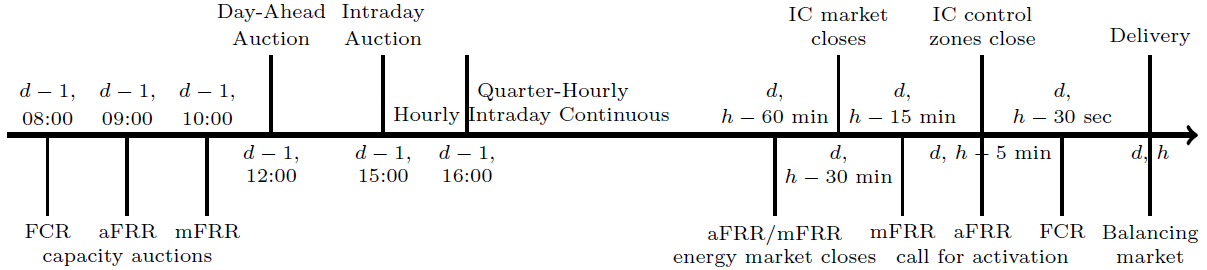
\includegraphics[width=\textwidth]{theory/energy_auctions.png}
            \caption[Timeschedule for energy market auctions]{Timeline of market auctions, intraday trading, and balancing energy activation leading up to delivery. Times are shown relative to delivery day 
d and hour 
h \cite{narajewskiProbabilisticForecastingGerman2022}.}
            \label{fig::energy_auctions}
 \end{figure}

Figure \ref{fig::energy_auctions} illustrates the auction and balancing sequence of the German electricity market, relative to the delivery timestamp (d, h).
The timeline begins on the previous day with three reserve capacity auctions:  \gls{FCR} at 08:00, aFRR at 09:00, and  \gls{mFRR} at 10:00. These auctions determine the prices for positive and negative balancing reserves, but since no data was available during this thesis, they are excluded from the analysis \cite{narajewskiProbabilisticForecastingGerman2022} .

The Day-Ahead auction follows at 12:00, and the Intraday Auction is held at 15:00.  \gls{IC} trading opens at 16:00 and continues until shortly before delivery. Unlike discrete auction events, \gls{IC} allows trading on a rolling basis \cite{EPEXTradingBrochure} \cite{narajewskiProbabilisticForecastingGerman2022} \cite{EPEXTradingBrochure}.

The \gls{IC} market closes in stages: cross-zone trades close 30 minutes before delivery, while trades within a single control zone remain possible until 5 minutes before delivery. This timestamp — 5 minutes before physical delivery — is referred to as the gate closure time throughout this thesis \cite{narajewskiProbabilisticForecastingGerman2022}  \cite{EPEXTradingBrochure}.

Understanding this market timing is essential, as it determines which information is available at prediction time, and directly influences both \gls{BRP} behavior and the imbalance price formation.

 
 
%On the far right of the figure the time of delivery is shown, denoted by $d$, $h$ of the delivery. The auctions for this timestamp start the day before. From $8:00$ to $10:00$ on the previous day reserve capacity auctions take place. These auctions decide the price for positive and negative balancing energy.
%Data about these auctions was not available at the time of this thesis, so no information about these auctions will be used throughout this thesis.
%The first auction takes place at $12:00$ one day before delivey and is called the day ahead (DA) auction. At $15:00$ the next auction, the intraday auction (IA) takes place. After that, at $16:00$ intraday continuous trading (IC) starts. Whilst the auctions are a single auction event, during the intraday continuous (IC) trading window energy can be traded at any time. The IC has different closing times. Up until $30$ minutes before delivery energy can be traded across all control zones. Trades on IC that happen within a single control zone can be done up until $5$ minutes before delivery.

%For the rest of the thesis the timestamp $5$ mintues before delivery time will be called the gate closure time.

%\subsection{Terminology}

%\subsubsection{Residual load}

%Residual load is the load  that has to be covered by not variable renewable energey (VRE) sources.
%It can be calculted by substracting the power produced by solar and wind (both off- and onshore) from the total load.

\section{Imbalance price}
\label{Section::Imbalance_Price}

 \begin{figure}[b]
            \centering
            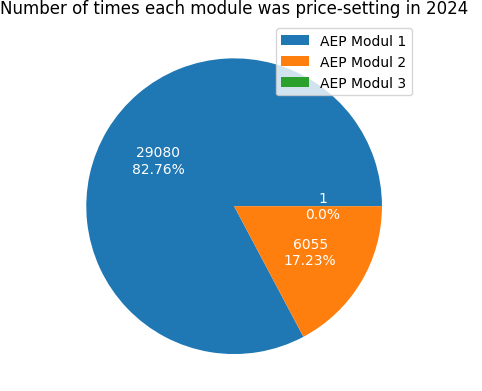
\includegraphics[width=.5\textwidth]{theory/aep_modules.pdf}
             \caption[How often each module was price-setting in 2024?]{How often each module was price-setting in 2024 \cite{NetztransparenzAEPModul}}
            \label{fig::aep_modules}
 \end{figure}
The German imbalance price — also referred to as the \gls{reBAP} — reflects the cost of balancing energy that \gls{BRP}s must pay or receive when their portfolio deviates from the submitted schedule.
To ensure consistency across control zones, a uniform price is calculated for all of Germany. The calculation is based on a modular approach defined by the \gls{TSO}s and regulatory framework \cite{NetztransparenzReBAPDefinition}.

The final imbalance price is determined from the results of three separate modules, each of which reflects a different aspect of the cost and incentive structure:
\begin{itemize}
\item Module 1: The cost of activated balancing reserves
\item Module 2: A market-based incentive to encourage portfolio balancing
\item Module 3: A scarcity signal in extreme imbalance situations
\end{itemize}
The module with the highest financial impact (depending on the sign of the system imbalance) is selected to define the \gls{reBAP} for each 15-minute settlement period. Figure \ref{fig::aep_modules} shows how often each module was price setting in 2024. Module 1 was price setting in 82,76\% and module 2 in 17,23\% of all quarter-hours\cite{NetztransparenzAEPModul}.



\subsection{Module 1: Basis component}
The basis component reflects the actual cost of activating balancing reserves. It serves as the default pricing module and is used in most settlement periods.
Two types of balancing reserves are considered:
\begin{itemize}
\item \gls{aFRR} 
\item \gls{mFRR} 
\end{itemize}

For each reserve, the \gls{VWAP} is calculated using data from the European platforms PICASSO (for \gls{aFRR}) and MARI (for \gls{mFRR}).
This results in four prices for each 15-minute interval:
\begin{itemize}
\item $VWAP_{aFRR}$ (positive and negative)
\item $VWAP_{mFRR}$ (positive and negative)
\end{itemize}

Depending on which reserve was activated, the system calculates the corresponding price ($AEP_1$). If both \gls{aFRR} and \gls{mFRR} were activated, a volume-weighted average of their \gls{VWAP}s is used.
If neither was activated, the avoided activation price is applied, typically computed as the average of the cheapest.

The resulting AEP₁ (either positive or negative) is selected based on the sign of the system balance (GCC balance)\cite{NetztransparenzReBAP}:
\begin{itemize}
\item If the system is short: the positive $AEP_1$ is used
\item If the system is long: the negative $AEP_1$ is used
\item If the system is balanced: the component is set to 0
\end{itemize}
%This module reflects the marginal cost of balancing and forms the foundation of the imbalance price in over 80\% of all intervals.




%The first module is called the basis component. 
%This module represents the cost of providing the balancing energy.

%With information provided by PICASSO the volume-weighted average price for the automatic frequency restoration reserve $VWAP_{aFRR}$ can be calculated. This is calculated for both positive and negative activations, resulting in $VWAP_{aFRR, GCC, pos, qh}$ and $VWAP_{aFRR,  GCC, neg, qh}$ for each quarter hour $qh$ and the GCC balance.
%The same calculations are done for mFRR activations using data from MARI, resulting int $VWAP_{mFRR, GCC, pos, qh}$ and $VWAP_{mFRR, GCC, neg, qh}$. 
%These valuese are used in the formulas \ref{fig::aep1_pos} and \ref{fig::aep1_neg} to calculate the values $AEP1_{pos}$ and $AEP1_{neg}$. 
%If neither aFRR or mFRR were activated during the associated quarter hour this $AEP1$ takes the value of avoided activation. This value is equal to the mean of the cheapest aFRR bid prices for the quarter hour.
%If only one of the reserves was activated $AEP1$ takes the value of the $VWAP$ of that reserve. 
%If both reserves were activated, the $AEP1$ is equal to the volume-weighted average of both $VWAPs$. The volume is denoted by the satisfied demand $SD$.

%\begin{figure}[ht]
%            \centering
%            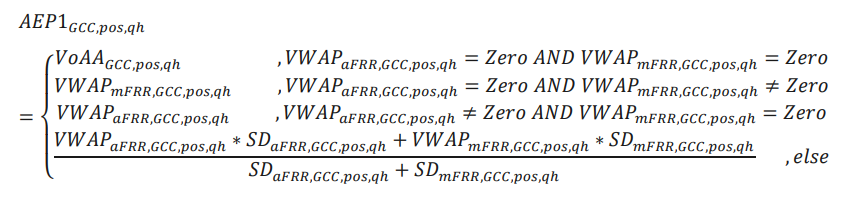
\includegraphics[width=\textwidth]{theory/aep1_pos.png}
%            \caption[Positive AEP 1 component formula]{Positive AEP 1 component formula %\cite{NetztransparenzReBAP}.}
%            \label{fig::aep1_pos}
% \end{figure}
 
 

% \begin{figure}[ht]
%            \centering
%            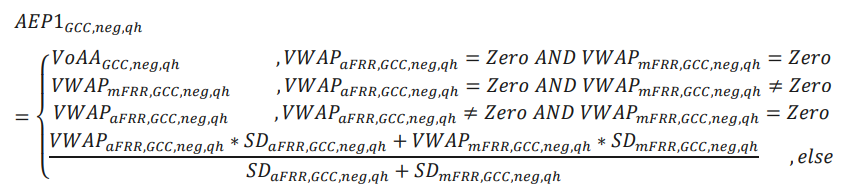
\includegraphics[width=\textwidth]{theory/aep1_neg.png}
%             \caption[Positive AEP 1 component formula]{Positive AEP 1 component formula %\cite{NetztransparenzReBAP}.}
%            \label{fig::aep1_neg}
% \end{figure}

%With both $AEP1s$, the value of the basis component can be calculated. If the system balance is positive, this module takes the value of $AEP1_{GCC, pos, qh}$. If the system balance is negative, this module takes the value of $AEP1_{GCC, neg, qh}$. If the system balance is equal to 0, this module's value is 0.

\subsection{Module 2: Incentivising component}
\label{Section::Module_2}
The incentivising component aims to discourage market participants from relying on imbalance energy and instead motivate them to actively balance their portfolios via intraday trading. The underlying idea is that imbalance energy should be more expensive than purchasing electricity directly on the market — especially shortly before delivery \cite{kochPASSIVEBALANCINGINTRADAY2020a} .

This module is applied only when there is sufficient liquidity in the intraday market for the quarter-hour in question. Specifically, the module is activated if the \gls{VID} for that interval exceeds 500 MW. If this threshold is not reached, the module is skipped, and its value is set to zero.

When activated, the \gls{ID AEP} serves as the reference point for calculating the \gls{reBAP}. This price is computed as the volume-weighted average of the most recent trades summing up to 500 MW (i.e., 125 MWh for a 15-minute period), executed as close as possible to the gate closure time.

To increase the incentive for \gls{BRP}s to remain balanced, the imbalance price is artificially adjusted by introducing a minimum price distance ($\Delta P$) between the \gls{reBAP} and the \gls{ID AEP}. This distance ramps up linearly with the absolute value of the \gls{GCC} system imbalance, up to a maximum value of 25\% of the \gls{ID AEP} — or at least €10/MWh, whichever is higher.

The logic can be summarized as follows:
\begin{itemize}
\item If the system is short (positive GCC balance):
 reBAP = ID AEP + $\Delta P$
\item If the system is long (negative GCC balance):
 reBAP = ID AEP − $\Delta P$
\item If the system is balanced:
 reBAP = ID AEP
\end{itemize}

$\Delta P$ is defined as a linear function of the GCC balance between 0 and ±500 MW. This relationship is visualized in Figure \ref{fig::delta_p_graph}, using a fixed ID AEP of €100/MWh as an example. 

From a forecasting perspective, Module 2 introduces a dynamic, nonlinear pricing logic. 
Since the final price is not directly based on \gls{ID AEP} alone, but also on the size and direction of the system imbalance, accurate forecasts of both \gls{GCC} balance and market prices are essential for reliable reBAP prediction during periods where this module is active.

In 2024, the incentivising component was the price-setting mechanism in 17.23\% of all 15-minute settlement intervals (Figure \ref{fig::aep_modules}). 
%These typically correspond to periods with moderate but directional imbalances, in which active trading signals are available near gate closure.

The next section discusses Module 3, which is triggered under conditions of extreme imbalance and scarcity of reserves.

%The goal behind module 2 is to increase the reBAP, so that it is more costly to use imbalance energy than buying the need energy on the intraday market. This should incentivise all BRPs to keep their portfolio balanced. 
%The formula for its calculation is displayed in figure \ref{fig::aep2}.and will be explained in the next paragraphs.

%For each settlement period $V_{ID}$ denotes the volume of total trades that were closed on the intraday market for this quarter. If this volume is below $500$MW, this component finds no application and takes the value of 0. If value was greater than $500$MW this module is calculated using the Intraday Price Index (ID AEP) and a minimum distance $\Delta P$. 
%The ID AEP is calculated for each quarter hour by averaging over the trades closest to the delivery time. For this calculation only a volume of 500 MW, so 125 MW/h for a quarter hour is considered.  
%The volume-weighted average price is formed from the transactions filtered this way. 
%In the case that the GCC balance is equal to 0, this module takes the value of ID AEP.  In the case of a positive GCC balance, a minimum distance $\Delta P$ is added onto the ID AEP, in case of a negative GCC balance this $\Delta P$ is substracted from the ID AEP. Between ID AEP and module 2 a minimum distance of $25\%$, but at least 10€ is established, assuming the absolute value of the GCC balance is equal to or greater than $500$ MW. This distance $\Delta P$ linearly ramps up from $0$MW to $500$MW. The formula for $\Delta P$ can be found in figure \ref{fig::delta_p} and a graph for its values with a fixed ID AEP of $100€/MWh$ is displayed in figure \ref{fig::delta_p_graph}.


 \begin{figure}[ht]
            \centering
            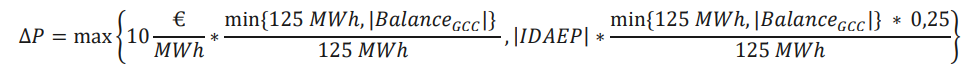
\includegraphics[width=.7\textwidth]{theory/delta_p.pdf}
             \caption[Graph for $\Delta P$ with a fixed ID AEP for $100€/MWh$]{Graph for $\Delta P$ with a fixed ID AEP for $100€/MWh$.}
            \label{fig::delta_p_graph}
 \end{figure}

 %\begin{figure}[ht]
%            \centering
%            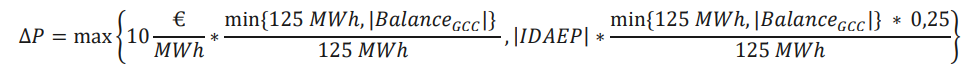
\includegraphics[width=\textwidth]{theory/delta_p.png}
%             \caption[Formula for$ \Delta P$]{Formula for $\Delta P$ .}
%            \label{fig::delta_p}
% \end{figure}
%  \begin{figure}[ht]
%            \centering
%            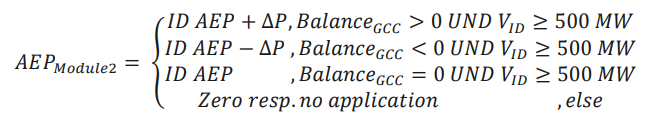
\includegraphics[width=\textwidth]{theory/aep_2.png}
%             \caption[Formula for $AEP_{Module 2}$]{Formula for $AEP_{Module 2}$.}
%            \label{fig::aep2}
% \end{figure}

\subsection{Module 3: Scarcity component}

%If the GCC balance exceeds $80\%$ of the frequency restoration reserve (FRR) for a settlement period, the scarcity component is applied. This component rarely is the price setting module of the reBAP (<1\%). The formula for this module will not be discussed here. Figure \ref{fig::aep_3} shows a graph of how this module's value changes relatively to the GCC balance.


% \begin{figure}[ht]
 %           \centering
  %          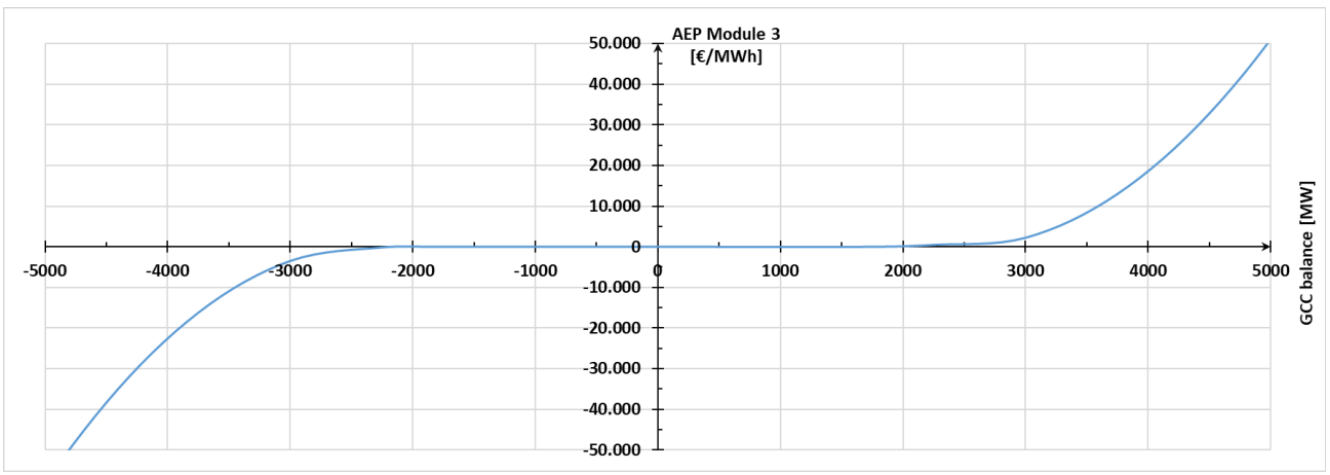
\includegraphics[width=\textwidth]{theory/aep_3.png}
%             \caption[Graph how the price of module 3 correlates with GCC balance]{Graph how the price of module 3 %correlates with GCC balance .}
%            \label{fig::aep_3}
% \end{figure}

The scarcity component is designed to reflect critical system conditions in which balancing reserves are nearly exhausted. It serves as an economic signal to incentivize all market participants to avoid any further deviation from their schedules under extreme imbalance situations.

This module is only activated if the \gls{GCC} balance (i.e., the aggregated system imbalance across all German control areas) exceeds 80\% of the available \gls{FRR} in a given settlement period. This threshold marks a high-stress scenario in which the grid approaches its technical limits for balancing energy provision.

When triggered, the scarcity component applies a penalty mechanism that leads to significantly higher imbalance prices compared to the other modules. However, due to its strict activation criteria, the module is rarely used in practice. In the year 2024, the scarcity component was the price-setting module in only one quarter-hour 

The exact formula for Module 3 is not discussed here, as its impact on overall \gls{reBAP} behavior is negligible from a statistical perspective. 
To provide an estimate of the values this module can take: in the one instance where Module 3 was price-setting in 2024, its value amounted to $10.097/MWh€$. 

Depending on the sign of the imbalance, the \gls{reBAP} is set to:
\begin{itemize}
\item the maximum of the three module values if the system is short (positive \gls{GCC} balance), or
\item the minimum if the system is long (negative \gls{GCC} balance)
\end{itemize}

This selection logic is applied uniformly across all modules. Figure \ref{fig::aep_modules} summarizes the percentage of intervals in 2024 in which each module determined the reBAP.
Even though Module 3 rarely sets the price, its existence serves as a critical backstop in the regulatory design — signaling the potential for extreme system stress and providing strong economic disincentives for imbalance during those periods.

%Depeding on the sign of the GCC balance, either the minimum or the maximum of the three modules introduced in the previous paragraphs is used. The formula for this is displayed in figure \ref{fig::rebap_neg}. If the GCC balance is positive, the module with the highest value is used. If the balance is negative the cheapest module is used to determine the reBAP.

%For the whole year 2024 the reBAP was equal to the basis component $82.76\%$, equal to the incentivising component $17.23\%$ and equal to the scarcity component $0.00\%$ of the time, with the scarcity component only being the price setting module once throughout 2024. This data is displayed in figure \ref{fig::aep_modules}.




% You can use this to add content for standalone documents if you like
% In this case we would like to show the references.
\ifstandalone
    % Bibliography
    \printbibliography[heading=bibintoc]                         \cleardoublepage

% ----------------------------------------------------------------------------
% Appendix and Glossary
% ----------------------------------------------------------------------------
%     \pagenumbering{Alph} % A, B, C..

% %     % Appendix
%     \documentclass[class=scrbook, crop=false]{standalone}
\usepackage[subpreambles=true]{standalone}
\ifstandalone
    % WARNING: Proceed with caution!

% -----------------------------------------------------------------------------------
% For package standalone
% -----------------------------------------------------------------------------------
\usepackage{import}

% -----------------------------------------------------------------------------------
% Language and typeset
% -----------------------------------------------------------------------------------
\usepackage[ngerman, english]{babel}

\usepackage{subcaption}
% Umlauts and other special characters (UTF-8)
% \usepackage[utf8]{inputenc}
\usepackage{fontspec}
\setsansfont{Arial}
% \usepackage[T1]{fontenc}  % Enable accented characters and umlauts
% LuaLatex doesn't need fontenc and uses UTF-8
% \usepackage{lmodern}  % Font face


% --------------------------------------------------------------------------------
% Page formatting
% --------------------------------------------------------------------------------
% Change the header/footer for chapter beginnings and normal pages
\usepackage[automark,headsepline]{scrlayer-scrpage}

% The package provides an easy and flexible user interface to customize the page
% layout, implementing auto-centering and auto-balancing mechanisms
% WARNING: WHEN CHANGING BCOR (Binding correction), the cover needs reworking!...
\newcommand{\theBCOR}{15mm}  % Define binding correction
\usepackage[
    bindingoffset=\theBCOR,
    % showframe, % Show boxes which indicate margins and paddings
    bottom = 3.5cm, % Margins
      left = 2.5cm,
     right = 2.5cm
] {geometry}

% The package 'float' provides a container for document objects which can not be
% broken over pages, such as tables and figures
% Needed for table and figure indexes  
\usepackage{float}

% support for landscape layout
\usepackage{lscape}

% support of \tablenotes command to add notes under table
\usepackage{threeparttable}

% To allow drawing more professional tables
\usepackage{booktabs}

% --------------------------------------------------------------------------------
% Contents
% --------------------------------------------------------------------------------
% Vector graphics (for Cover page)
\usepackage{tikz} 

% Allows additional parameters when including images
\usepackage{graphicx}

% Roman font family for all headings
\addtokomafont{disposition}{\rmfamily}

% Set the line spacing to 1.5
\usepackage[onehalfspacing]{setspace}

% Improves overall text spacing
% http://www.khirevich.com/latex/microtype/
\usepackage[stretch=10]{microtype}

% Math symbols like mu outside the math environment
\usepackage{textcomp}

% A comprehensive (SI) units package∗
% For defining SI units
\usepackage[
    range-units=single,         % Formatting ranges with single unit indication: 1 - 2 m
    range-phrase=-,             % Phrase for range: 1 - 2 m vs 1 to 2 m
    separate-uncertainty=true,  % sets +- between value and uncertainty 
    multi-part-units=repeat     % In expressions with multiple values (multi part numbers) 
                                % the unit is printed each time: 1 mm x 1 mm
] {siunitx}
% https://tex.stackexchange.com/questions/124488/multi-part-numbers-and-units-in-siunitx

% Allows Sourcecodes with highlighting 
\usepackage{listings}

% This package provides user control over the layout of the three basic list
% environments: enumerate, itemize and description
\usepackage{enumitem}
\setlist{nosep} % Remove the vertical space between \item elements in all lists

% ToDo Notes
% \setlength{\marginparwidth}{2cm}
\usepackage{todonotes}
\setuptodonotes{inline, inlinepar}
\reversemarginpar  % Put ToDo notes on the binding's side
% \usepackage{soul} % Colorful ToDo notes

% Check out colors here http://latexcolor.com/
\usepackage{xcolor}

\usepackage{amsmath}    % alignment of equations

% --------------------------------------------------------------------------------
% Other elements
% --------------------------------------------------------------------------------
% Blindtext: Organic looking text dummy
\usepackage{blindtext}

% Hyperlinks within the document (PDF)
% "hidelinks" hides visual highlighting of links
\usepackage[hidelinks]{hyperref}

% Package for Glossary and Index (Acronyms are listed in a separate list) 
\usepackage[acronym, nogroupskip]{glossaries}[=v4.49] % groupskip: alphabetic grouping of entries

\usepackage{xltabular}   % <------- FOR glossaries

% Integration and management of bibliographies
\usepackage{csquotes}   % backend=biber in biblatex needs this package
\usepackage[
    style=ieee,   % style of the bibliography, entries are sorted in alphabetic order. "ieee" is another common style.
    backend=biber,      % based on package 'biber' 
    bibencoding=ascii   % ASCII Text encoding; may use "utf8" instead
] {biblatex}

% --------------------------------------------------------------------------------
%                               PATHS & FILES
% --------------------------------------------------------------------------------
% Fix paths for standalone compiling
\ifstandalone
    \def \home {..}
\else
    \def \home {.}
\fi

% Package: scrlayer-scrpage
% \def \stylePath {\home/settings+/style/page}
\input{\home/settings+/style/page}  % Load page style

% Package: graphicx
\graphicspath{{\home/images/}}  % Set path to images

% Package: listings
\input{\home/settings+/style/code.tex}  % Set path to style file
\lstset{inputpath={\home/code/}} % Default path to code listings

% Package: glossaries
\input{\home/settings+/style/symbols}  % Set path to symbols list style file
\input{\home/settings+/style/acronyms}  % Set path to acronym list style file
\input{\home/references/glossary_acronyms}  % Load glossary, symbol and acronyms list

% Package: biblatex
\addbibresource{\home/references/references.bib}  % Set path to bib resources

% Custom variables
\input{\home/settings+/variables}
% --------------------------------------------------------------------------------
%                                   OPTIONAL
% --------------------------------------------------------------------------------


% Simple arithmetic for LaTeX commands
% \usepackage{calc}

% Document Elements
% -------------------

% Index
% \usepackage{imakeidx}

% compact Lists
%\usepackage{paralist}

% visual improvements for citations
% \usepackage{epigraph}

% Create pseudo code
% https://www.overleaf.com/learn/latex/Algorithms
% \usepackage{algorithm}
% \usepackage{algorithmic}
%\usepackage[noend]{algpseudocode}

% Formatting
% -------------------
% Tweaks for scrbook, redefines commands of other packages
% \usepackage{scrhack}

% Intelligent space separator (nice for superscript?)
% \usepackage{xspace}

% Allows breaks within tables
%\usepackage{tabularx}

% Allows for page breaks in tables
% \usepackage{longtable}

% allows modifying of captions
% \usepackage{caption}

% Multiline comments
%\usepackage{verbatim}

% % Custom colors
% \definecolor{dartmouthgreen}{rgb}{0.05, 0.5, 0.06}

% IF you want to define unicode characters
% \DeclareUnicodeCharacter{0229}{\c{e}}
% \DeclareUnicodeCharacter{0306}{\u{Z}}


% Document elements
% ------------------------------------

% Table package
% \usepackage{booktabs}

% Pie diagram
% \usepackage{datapie}

% Side by Side images
% \usepackage{subcaption}

% For landscape tables
%\usepackage{pdflscape}
%\usepackage{afterpage}

% Graphics can be flow around by text
%\usepackage{wrapfig}

\fi

% ----------------------------------------------------------------------------
%                                 Appendix
% ----------------------------------------------------------------------------
\begin{document}
\appendix

\chapter{}
\addcontentsline{toc}{chapter}{Some Appendix}
\label{Chapter::Some Appendix}
Stuff that was not important or too much for the thesis but is still important or complements the presented results.

\section{Section A}
\label{Section::Some Appendix:Section A}


\begin{table}[]
\begin{tabular}{l|l}
Parameter & Description \\\hline
 ABSF\_STD & Hourly value for absolute humidity \\
   D & Wind direction\\
   F & Wind speed\\
   FF & Wind speed (10 minute average)\\
 FX\_911	& Fastest gust of wind in the last hour \\
   P	& Air pressure at NN \\
   P0	 & Air pressure at Station \\
   P\_STD & Hourly value for air pressure \\
   R1 & Hourly precipitation height \\
   RF\_STD	& Hourly value for relative humidity \\
   RF\_TU & Relative humidity \\
   RS\_IND	& Precipitation indicator (yes/no) \\
   SD\_SO	 & Hourly sunshine duration \\
   TD	 & Dew point temperature \\
   TD\_STD	& Dew point temperature in 2m height\\
   TF\_STD & Hourly value for humidity temperature\\
   TT	 & Temperature in 2m height \\
   TT\_TU & Air temperature \\
   V\_N & Cloud coverage (all clouds) \\
   V\_S1\_CS	 & Cloud type (first layer) \\
   V\_S1\_CSA & Cloud type abbreviation (first layer) \\
   V\_S1\_HHS	& Cloud height (first layer) \\
   V\_S1\_NS	 & Cloud coverage (first layer) \\
   V\_S2\_CS & Cloud type (second layer) \\
   V\_S2\_CSA & Cloud type abbreviation (second layer) \\
   V\_S2\_HHS	& Cloud height (second layer) \\
   V\_S2\_NS	 & Cloud coverage (second layer) \\
   V\_S3\_CS & Cloud type (third layer) \\
   V\_S3\_CSA & Cloud type abbreviation (third layer) \\
   V\_S3\_HHS	& Cloud height (third layer) \\
   V\_S3\_NS	 & Cloud coverage (third layer) \\
   V\_S4\_CS & Cloud type (fourth layer) \\
   V\_S4\_CSA & Cloud type abbreviation (fourth layer) \\
   V\_S4\_HHS	& Cloud height (fourth layer) \\
   V\_S4\_NS	 & Cloud coverage (fourth layer) \\
   V\_VV	& Visibility\\
  
   WRTR & Hourly Precipitaion form \\
   WW & Hourly observed weather \\ 
   
\end{tabular}
\caption{Variables in DWD measurement data}
\label{Table::DWD_Measurement_Parameters}
\end{table}


\begin{table}[]
\begin{tabular}{l|l}
Parameter & Description \\\hline
DD & Wind direction\\
FF & Wind speed\\
FX1 & Maximum wind gust within the last hour\\
FX3 & Maximum wind gust within the last 3 hours\\
FXh & Maximum wind gust within the last 12 hours\\
FXh25 & Probability of wind gusts >= 25kn within the last 12 hours\\
FXh40 & Probability of wind gusts >= 40kn within the last 12 hours\\
FXh55 & Probability of wind gusts >= 55kn within the last 12 hours\\
N & Total cloud cover\\
N05 & Cloud cover below 500 ft.\\
Neff & Effective cloud cover\\
Nh & High cloud cover (>7 km)\\
Nl & Low cloud cover (lower than 2 km)\\
Nm & Midlevel cloud cover (2-7 km)\\
PPPP & Surface pressure, reduced\\
R602 & Probability of precipitation > 0.2mm during the last 6 hours\\
R650 & Probability of precipitation > 5.0mm during the last 6 hours\\
RR1c & Total precipitation during the last hour consistent with significant weather\\
RR3c & Total precipitation during the last 3 hours consistent with significant weather\\
RRS1c & Snow-Rain-Equivalent during the last hour\\
RRS3c & Snow-Rain-Equivalent during the last 3 hours\\
Rad1h & Global Irradiance\\
Rd02 & Probability of precipitation > 0.2mm during the last 24 hours\\
Rd50 & Probability of precipitation > 5.0mm during the last 24 hours\\
Rh00 & Probability of precipitation > 0.0mm during the last 12 hours\\
Rh02 & Probability of precipitation > 0.2mm during the last 12 hours\\
Rh10 & Probability of precipitation > 1.0mm during the last 12 hours\\
Rh50 & Probability of precipitation > 5.0mm during the last 12 hours\\
SunD1 & Sunshine duration during the last Hour\\
T5cm & Temperature 5cm above surface\\
TN & Minimum temperature - within the last 12 hours\\
TTT & Temperature 2m above surface\\
TX & Maximum temperature - within the last 12 hours\\
Td & Dewpoint 2m above surface\\
VV & Visibility\\
W1W2 & Past weather during the last 6 hours\\
ww & Significant Weather\\
wwM & Probability for fog within the last hour\\
wwM6 & Probability for fog within the last 6 hours\\
wwMh & Probability for fog within the last 12 hours\\
\end{tabular}
\caption{Variables in DWD MOSMIX data}
\label{Table::DWD_MOSMIX_Parameters}
\end{table}

\subsection{Subsection B}
\label{Subsection::Some Appendix:Subsection B}

\Blindtext
\chapter{}
\addcontentsline{toc}{chapter}{Some Appendix2}

\blindtext
\Blindtext

\end{document}
                                          \clearpage

% %     % Symbol list also counts as a glossary object
%     \printglossary[type=main]  % main glossary

% %     % Either print all entries or only used entries for all lists
%     \glsaddallunused
\fi

\end{document}
                                               \clearpage
    \documentclass[class=scrbook, crop=false]{standalone}
\usepackage[subpreambles=true]{standalone}
\ifstandalone
    % WARNING: Proceed with caution!

% -----------------------------------------------------------------------------------
% For package standalone
% -----------------------------------------------------------------------------------
\usepackage{import}

% -----------------------------------------------------------------------------------
% Language and typeset
% -----------------------------------------------------------------------------------
\usepackage[ngerman, english]{babel}

\usepackage{subcaption}
% Umlauts and other special characters (UTF-8)
% \usepackage[utf8]{inputenc}
\usepackage{fontspec}
\setsansfont{Arial}
% \usepackage[T1]{fontenc}  % Enable accented characters and umlauts
% LuaLatex doesn't need fontenc and uses UTF-8
% \usepackage{lmodern}  % Font face


% --------------------------------------------------------------------------------
% Page formatting
% --------------------------------------------------------------------------------
% Change the header/footer for chapter beginnings and normal pages
\usepackage[automark,headsepline]{scrlayer-scrpage}

% The package provides an easy and flexible user interface to customize the page
% layout, implementing auto-centering and auto-balancing mechanisms
% WARNING: WHEN CHANGING BCOR (Binding correction), the cover needs reworking!...
\newcommand{\theBCOR}{15mm}  % Define binding correction
\usepackage[
    bindingoffset=\theBCOR,
    % showframe, % Show boxes which indicate margins and paddings
    bottom = 3.5cm, % Margins
      left = 2.5cm,
     right = 2.5cm
] {geometry}

% The package 'float' provides a container for document objects which can not be
% broken over pages, such as tables and figures
% Needed for table and figure indexes  
\usepackage{float}

% support for landscape layout
\usepackage{lscape}

% support of \tablenotes command to add notes under table
\usepackage{threeparttable}

% To allow drawing more professional tables
\usepackage{booktabs}

% --------------------------------------------------------------------------------
% Contents
% --------------------------------------------------------------------------------
% Vector graphics (for Cover page)
\usepackage{tikz} 

% Allows additional parameters when including images
\usepackage{graphicx}

% Roman font family for all headings
\addtokomafont{disposition}{\rmfamily}

% Set the line spacing to 1.5
\usepackage[onehalfspacing]{setspace}

% Improves overall text spacing
% http://www.khirevich.com/latex/microtype/
\usepackage[stretch=10]{microtype}

% Math symbols like mu outside the math environment
\usepackage{textcomp}

% A comprehensive (SI) units package∗
% For defining SI units
\usepackage[
    range-units=single,         % Formatting ranges with single unit indication: 1 - 2 m
    range-phrase=-,             % Phrase for range: 1 - 2 m vs 1 to 2 m
    separate-uncertainty=true,  % sets +- between value and uncertainty 
    multi-part-units=repeat     % In expressions with multiple values (multi part numbers) 
                                % the unit is printed each time: 1 mm x 1 mm
] {siunitx}
% https://tex.stackexchange.com/questions/124488/multi-part-numbers-and-units-in-siunitx

% Allows Sourcecodes with highlighting 
\usepackage{listings}

% This package provides user control over the layout of the three basic list
% environments: enumerate, itemize and description
\usepackage{enumitem}
\setlist{nosep} % Remove the vertical space between \item elements in all lists

% ToDo Notes
% \setlength{\marginparwidth}{2cm}
\usepackage{todonotes}
\setuptodonotes{inline, inlinepar}
\reversemarginpar  % Put ToDo notes on the binding's side
% \usepackage{soul} % Colorful ToDo notes

% Check out colors here http://latexcolor.com/
\usepackage{xcolor}

\usepackage{amsmath}    % alignment of equations

% --------------------------------------------------------------------------------
% Other elements
% --------------------------------------------------------------------------------
% Blindtext: Organic looking text dummy
\usepackage{blindtext}

% Hyperlinks within the document (PDF)
% "hidelinks" hides visual highlighting of links
\usepackage[hidelinks]{hyperref}

% Package for Glossary and Index (Acronyms are listed in a separate list) 
\usepackage[acronym, nogroupskip]{glossaries}[=v4.49] % groupskip: alphabetic grouping of entries

\usepackage{xltabular}   % <------- FOR glossaries

% Integration and management of bibliographies
\usepackage{csquotes}   % backend=biber in biblatex needs this package
\usepackage[
    style=ieee,   % style of the bibliography, entries are sorted in alphabetic order. "ieee" is another common style.
    backend=biber,      % based on package 'biber' 
    bibencoding=ascii   % ASCII Text encoding; may use "utf8" instead
] {biblatex}

% --------------------------------------------------------------------------------
%                               PATHS & FILES
% --------------------------------------------------------------------------------
% Fix paths for standalone compiling
\ifstandalone
    \def \home {..}
\else
    \def \home {.}
\fi

% Package: scrlayer-scrpage
% \def \stylePath {\home/settings+/style/page}
\input{\home/settings+/style/page}  % Load page style

% Package: graphicx
\graphicspath{{\home/images/}}  % Set path to images

% Package: listings
\input{\home/settings+/style/code.tex}  % Set path to style file
\lstset{inputpath={\home/code/}} % Default path to code listings

% Package: glossaries
\input{\home/settings+/style/symbols}  % Set path to symbols list style file
\input{\home/settings+/style/acronyms}  % Set path to acronym list style file
% -------------------------------------------------------------------------------
%               Listing of all Glossary and Acronym Entries 
%                           use as shown below
% -------------------------------------------------------------------------------

% ==== EXEMPLARY ENTRY FOR SYMBOLS LIST =========================================

% ==== EXEMPLARY ENTRY FOR ACRONYMS LIST ========================================
% \newacronym{#label}{#acronym}{#long_form}

% define new command for custom arconym entry with only two arguments
% fabricates an easier way to use \newacronym 
\newcommand{\acroX}[2]{\newacronym{#1}{#1}{#2}}
% \acroX{label and arconym}{long name}
% \acroX{CD}               {Compact Disk}

\newcommand{\acroY}[3]{\newacronym{#1}{#2}{#3}}
% \arcoY{label}{acronym}{long name}
% \acroY{CD}   {cd}     {Compact Disk}
 
\newacronym{AEP}{AEP}{Imbalance price}
\newacronym{aFRR}{aFRR}{Automatic Frequency Restoration Reserve}


\newacronym{reBAP}{reBAP}{Uniform imbalance price}
\newacronym{TSO}{TSO}{Transmission System Operator}
\newacronym{FCR}{FCR}{Frequency Containment Reserve}
\newacronym{mFRR}{mFRR}{Manual Frequency Restoration Reserve}
\newacronym{BRP}{BRP}{Balancing Responsible Party}
\newacronym{SB}{SB}{System Balance}
\newacronym{VRE}{VRE}{variable renewable energy}
\newacronym{ID1}{ID1}{intraday index ID1}
\newacronym{MAE}{MAE}{mean average error}
\newacronym{RMSE}{RMSE}{root mean squared error}
\newacronym{MSE}{MSE}{mean squared error}
\newacronym{CRPS}{CRPS}{continuous ranked probabililty score}
\newacronym{GCC}{GCC}{Grid Control Cooperation}
\newacronym{IC}{IC}{Continuous intraday}
\newacronym{VWAP}{VWAP}{volume-weighted average price}
\newacronym{VID}{VID}{traded volume within the intraday market}
\newacronym{ID AEP}{ID AEP}{Intraday Average Energy Price}
\newacronym{FRR}{FRR}{Frequency Restoration Reserve}
\newacronym{TFT}{TFT}{Temporal Fusion Transformer}
\newacronym{DLM}{DLM}{Dynamic Linear Model}
\newacronym{GB}{GB}{Gradient Boosting}
\newacronym{RF}{RF}{Random Forest}
\newacronym{ARIMAX}{ARIMAX}{Autoregressive Integrated Moving Average with eXogenous variables}
\newacronym{xLSTM}{xLSTM}{Extended Long Short-Term Memory}
\newacronym{DWD}{DWD}{Deutscher Wetterdienst}
\newacronym{ENTSO-E}{ENTSO-E}{European Network of Transmission System Operators for Electricity}
\newacronym{IDA1}{IDA1}{Intraday auction 1}
\newacronym{MOSMIX}{MOSMIX}{Model Output Statistics-MIX}
\newacronym{mLSTM}{mLSTM}{memory-optimized LSTM}
\newacronym{sLSTM}{sLSTM}{speed-optimized LSTM}

% ==== EXEMPLARY ENTRY FOR MAIN GLOSSARY ========================================

    % \newglossaryentry{policy}{name={Policy},description={Im geschäftlichen Bereich bezeichnet Policy eine interne Leit- bzw. Richtlinie, die formal durch das Unternehmen dokumentiert und über ihr Management verantwortet wird}}
    % \newglossaryentry{pcie}{name={PCI Express},description={PCI Express („Peripheral Component Interconnect Express“, abgekürzt PCIe oder PCI-E) ist ein Standard zur Verbindung von Peripheriegeräten mit dem Chipsatz eines Hauptprozessors. PCIe ist der Nachfolger von PCI, PCI-X und AGP und bietet im Vergleich zu seinen Vorgängern eine höhere Datenübertragungsrate pro Pin.}}
    % \newglossaryentry{realnumber}
  % Load glossary, symbol and acronyms list

% Package: biblatex
\addbibresource{\home/references/references.bib}  % Set path to bib resources

% Custom variables
\input{\home/settings+/variables}
% --------------------------------------------------------------------------------
%                                   OPTIONAL
% --------------------------------------------------------------------------------


% Simple arithmetic for LaTeX commands
% \usepackage{calc}

% Document Elements
% -------------------

% Index
% \usepackage{imakeidx}

% compact Lists
%\usepackage{paralist}

% visual improvements for citations
% \usepackage{epigraph}

% Create pseudo code
% https://www.overleaf.com/learn/latex/Algorithms
% \usepackage{algorithm}
% \usepackage{algorithmic}
%\usepackage[noend]{algpseudocode}

% Formatting
% -------------------
% Tweaks for scrbook, redefines commands of other packages
% \usepackage{scrhack}

% Intelligent space separator (nice for superscript?)
% \usepackage{xspace}

% Allows breaks within tables
%\usepackage{tabularx}

% Allows for page breaks in tables
% \usepackage{longtable}

% allows modifying of captions
% \usepackage{caption}

% Multiline comments
%\usepackage{verbatim}

% % Custom colors
% \definecolor{dartmouthgreen}{rgb}{0.05, 0.5, 0.06}

% IF you want to define unicode characters
% \DeclareUnicodeCharacter{0229}{\c{e}}
% \DeclareUnicodeCharacter{0306}{\u{Z}}


% Document elements
% ------------------------------------

% Table package
% \usepackage{booktabs}

% Pie diagram
% \usepackage{datapie}

% Side by Side images
% \usepackage{subcaption}

% For landscape tables
%\usepackage{pdflscape}
%\usepackage{afterpage}

% Graphics can be flow around by text
%\usepackage{wrapfig}

\fi

% ----------------------------------------------------------------------------
%                               State of the Art
% ----------------------------------------------------------------------------
\begin{document}

\chapter{State of the Art}
\label{Chapter::State_of_the_Art} % Outline text

In this chapter models and papers for the prediction of the german imbalance price as well as general time series predictors will be discussed. 
With this information I will conclude this chapter by showing how this thesis fits into the current ecosystem.

% Topics that are similar to yours but are already published.
% Explain their approach and what the difference to your approach is.
\section{Related Work}
\label{Section::Related_Work}

Several other papers have worked on forecasting on the imbalance market. Different energy markets are structured differently. While the imbalance is settled every quarter hour in germany \cite{narajewskiProbabilisticForecastingGerman2022}, each settlement period is 30 minutes on the energy market in the united kingdom \cite{limaBayesianPredictiveDistributions2023}.


The works \cite{limaBayesianPredictiveDistributions2023} \cite{ganeshForecastingImbalancePrice2024} \cite{garciaForecastingSystemImbalance2006} \cite{browellPredictingElectricityImbalance2022} \cite{lucasPriceForecastingBalancing2020} \cite{dengSeasonalityDeepLearning2024} focus on the energy market in the united kingdom and use different approaches. While \cite{limaBayesianPredictiveDistributions2023}, \cite{ganeshForecastingImbalancePrice2024}, \cite{browellPredictingElectricityImbalance2022}, \cite{lucasPriceForecastingBalancing2020} and \cite{dengSeasonalityDeepLearning2024} try to make a prediction about the imbalance price, \cite{garciaForecastingSystemImbalance2006} tries to forecast the total imbalance volume. 

The volume is forecasted using three different methods, ARIMA, exponential smoothing and caterpillar forecasting.

For the papers predicting imbalance prices different models where used.
The authors of \cite{limaBayesianPredictiveDistributions2023} developped a dynamic linear model (DLM) and compared their results to GARCH and AR-GARCH. Their model outperformed GARCH and AR-GARCH on all their out-of-sample forecasting experiments. During their research they also look at how the imbalance price correlated with different error values.
In \cite{ganeshForecastingImbalancePrice2024} many different neural network algorithms were compared, namely Recurrent Neural Networks (RNN), Long Short Term Memory (LSTM), Gated Recurrent Units (GRU), Temporal Fusion Transformer (TFT), Fully Connected Neural Networks (FCNN) and the Neural basis expansion analysis for interpretable time series forecasting (N-BEATS). The FCNNs used in this paper were a significant improvement to the DLM developed in \cite{limaBayesianPredictiveDistributions2023}.
The authors of \cite{browellPredictingElectricityImbalance2022} investigated how much impact the prediction time has on the result. They used Kernel Density Estimators (KDE) and linear regression to get a forecast for the imbalance price. 
 
 For the imbalance price prediction \ref{lucasPriceForecastingBalancing2020} employed Gradient Boosting (GB), Random Forest (RF) and XGBoost. Out of the models they used RF performed the best. During their research they also looked into feature importance for all their models. They found that the net imbalance volume was the most important feature.
 
 In \cite{dengSeasonalityDeepLearning2024} a new Bidirectional LSTM (BiLSTM) and Seasonal Attention BiLSTM (SA-BiLSTM) were compared to the previously used models. The authors looked into forecasting for multiple settlement periods into the future, with SA-BiLSTM performing the best in most of the cases.
 
Apart from the UK energy market some research on the Belgian \cite{bottieauVeryShortTermProbabilisticForecasting2020} \cite{dumasProbabilisticForecastingImbalance2019}, Hungarian \cite{balazsShorttermSystemImbalance2024} and German \cite{narajewskiProbabilisticForecastingGerman2022} electricity market was published.
In the papers \cite{bottieauVeryShortTermProbabilisticForecasting2020} and \cite{balazsShorttermSystemImbalance2024} the authors used machine learning methods and auto regressive methods to predict the system imbalance in their respective energy market.
A two step probabilistic approach was suggested in \cite{dumasProbabilisticForecastingImbalance2019}. First the system imbalance is forecasted and this information is then used in a second prediction for the imbalance price.

The paper on the german electricity market \cite{narajewskiProbabilisticForecastingGerman2022} used lasso regression, gamlss and a probabilistic neural network (PNN) to try to predict the imbalance price for the german electricity market. The data for their models was split into subsets and different models with different hyperparameter configurations trained for each subset.

Many of the mentioned papers, especially the ones on the british electricity market used data from before the COVID-19 pandemic. During the pandemic the energy market changed. Models based and calibrated on pre-pandemic data can not be used to effectively forecast current energy prices \cite{abadieEnergyMarketPrices2021}.


In this thesis different models are compared on the task of predicting the imbalance price. For this task models will be used that performed well pre-pandemic (RF) as well as an alteration on LSTM called xLSTM \cite{beckXLSTMExtendedLong2024} and a new inverted Transformer (iTransformer) \cite{liuITransformerInvertedTransformers2023} architecture.


\section{Time Series Predictors}
\label{Section::Time_Series_Predictors}

In this thesis established machine learning models are compared with novel approaches for Time Series Predictors. These newer models will be introduced in the next two subsections.

%\subsection{ARIMA}
%\label{Section::ARIMA}

%\subsection{Random Forest}
%\label{Section::Random_Forest}


\subsection{xLSTM}
\label{Section::xLSTM}
Extended Long Short-Term Memory (xLSTM) is a novel model which is based on the existing Long Short-Term Memory (LSTM) \cite{gravesLongShortTermMemory2012}. The recent advances in Transformer technology outperformed LSTM models. This alteration on the LSTM model extends  the amount of parameters by introducing new LSTM cells. 
These two new cells are the sLSTM and mLSTM cell.

In the sLSTM Cell the activation function is changed. While in LSTM the activation function for the input gate is the sigmoid function, sLSTM uses the exponential function. In sLSTM the activation for the forget gate can be either the sigmoid function or the exponential function. sLSTM cells can also have multiple memory cells. This enables memory mixing via recurrent connections. A residual sLSTM cell contains a sLSTM  cell which summarizes the past in the original space. This is then linearly mapped into a higher-dimensional  space where the non linear activation function is applied. Afterwards the result is mapped back to the original space.

The second alteration of the basic LSTM cell uses a matrix memory instead of a single value. This cell is called mLSTM. It also uses exponential gating for the input gate and either sigmoid or exponential gating for the forget gate. This cell can also have multiple memorry cells, but does not support memory mixing. In a residual mLSTM cell a pre-projection linearly maps to a high-dimensional space. The mLSTM cell then summarizes the past in the high dimensional space. The result is then linearly mapped back to the original space.

An xLSTM architecture is constructed by stacking theses building blocks. An advantage of xLSTM networks is, that the computation complexity is linear and the memory complexity is constant with respect to sequence length. \cite{beckXLSTMExtendedLong2024}



\subsection{iTransformer}
\label{Section::iTransformer}

Contrary to traditional Transformers, inverted Transformers (iTransformer) use inverted inputs. Transformers use temporal embedded tokens, learning one embedding for each distinct timestep across all variates. In iTransformers the input is transposed, changing the axes. This results in each embedding being learned for a single variate across all timesteps. For traditional Transformers the amount of learned embeddings is equal to the amount of timesteps, whereas for iTransformers the amount of learned embeddings is equal to the variates. This is visualized in figure \ref{fig::iTransformer}.

\begin{figure}[ht]
            \centering
            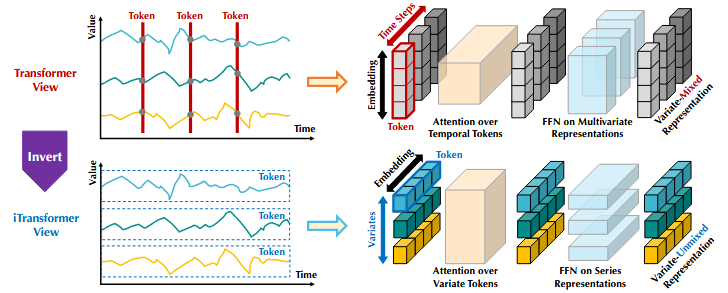
\includegraphics[width=\textwidth]{sota/iTransformer.png}
            \caption[Comparison between vanilla Transformer and iTransformer \cite{liuITransformerInvertedTransformers2023}]{Comparison between vanilla Transformer and iTransformer \cite{liuITransformerInvertedTransformers2023}}
            \label{fig::iTransformer}
 \end{figure}
 
The gains of inverting the input is significant. In the experiments the developers of the iTransformer found, that inverting the input had a benefit for various Transformers, namely the vanilla Transformer, Reformer, Informer, Flowformer and Flashformer. 
This research was done on weather data, traffic data and data about the hourly electricity consumption (ECL).
For the training of the iTransformer an updated training procedure was applied. 
For each batch only a subset of the variates are selected and the model is trained on them. 
The updated training process is a lot fasater, while the performance is still comparable with full-variate training. 
Another benefit of this training method is that the needed memory can be reduced significantly as shown in figure \ref{fig::iTransformer_Training} \cite{liuITransformerInvertedTransformers2023}

\begin{figure}[ht]
            \centering
            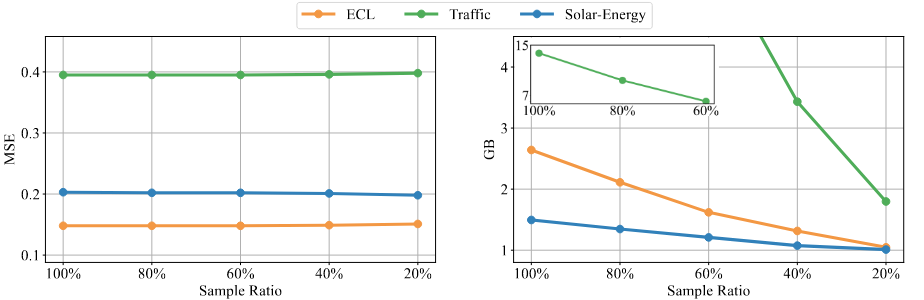
\includegraphics[width=\textwidth]{sota/iTransformer_Training.png}
            \caption[Training Performance (left) and training memory footprint (right) for training on only a subset of variates \cite{liuITransformerInvertedTransformers2023}]{Training Performance (left) and training memory footprint (right) for training on only a subset of variates \cite{liuITransformerInvertedTransformers2023}}
            \label{fig::iTransformer_Training}
 \end{figure}

\end{document}


                                                 \clearpage
    \documentclass[class=scrbook, crop=false]{standalone}
\usepackage[subpreambles=true]{standalone}
\ifstandalone
    % WARNING: Proceed with caution!

% -----------------------------------------------------------------------------------
% For package standalone
% -----------------------------------------------------------------------------------
\usepackage{import}

% -----------------------------------------------------------------------------------
% Language and typeset
% -----------------------------------------------------------------------------------
\usepackage[ngerman, english]{babel}

\usepackage{subcaption}
% Umlauts and other special characters (UTF-8)
% \usepackage[utf8]{inputenc}
\usepackage{fontspec}
\setsansfont{Arial}
% \usepackage[T1]{fontenc}  % Enable accented characters and umlauts
% LuaLatex doesn't need fontenc and uses UTF-8
% \usepackage{lmodern}  % Font face


% --------------------------------------------------------------------------------
% Page formatting
% --------------------------------------------------------------------------------
% Change the header/footer for chapter beginnings and normal pages
\usepackage[automark,headsepline]{scrlayer-scrpage}

% The package provides an easy and flexible user interface to customize the page
% layout, implementing auto-centering and auto-balancing mechanisms
% WARNING: WHEN CHANGING BCOR (Binding correction), the cover needs reworking!...
\newcommand{\theBCOR}{15mm}  % Define binding correction
\usepackage[
    bindingoffset=\theBCOR,
    % showframe, % Show boxes which indicate margins and paddings
    bottom = 3.5cm, % Margins
      left = 2.5cm,
     right = 2.5cm
] {geometry}

% The package 'float' provides a container for document objects which can not be
% broken over pages, such as tables and figures
% Needed for table and figure indexes  
\usepackage{float}

% support for landscape layout
\usepackage{lscape}

% support of \tablenotes command to add notes under table
\usepackage{threeparttable}

% To allow drawing more professional tables
\usepackage{booktabs}

% --------------------------------------------------------------------------------
% Contents
% --------------------------------------------------------------------------------
% Vector graphics (for Cover page)
\usepackage{tikz} 

% Allows additional parameters when including images
\usepackage{graphicx}

% Roman font family for all headings
\addtokomafont{disposition}{\rmfamily}

% Set the line spacing to 1.5
\usepackage[onehalfspacing]{setspace}

% Improves overall text spacing
% http://www.khirevich.com/latex/microtype/
\usepackage[stretch=10]{microtype}

% Math symbols like mu outside the math environment
\usepackage{textcomp}

% A comprehensive (SI) units package∗
% For defining SI units
\usepackage[
    range-units=single,         % Formatting ranges with single unit indication: 1 - 2 m
    range-phrase=-,             % Phrase for range: 1 - 2 m vs 1 to 2 m
    separate-uncertainty=true,  % sets +- between value and uncertainty 
    multi-part-units=repeat     % In expressions with multiple values (multi part numbers) 
                                % the unit is printed each time: 1 mm x 1 mm
] {siunitx}
% https://tex.stackexchange.com/questions/124488/multi-part-numbers-and-units-in-siunitx

% Allows Sourcecodes with highlighting 
\usepackage{listings}

% This package provides user control over the layout of the three basic list
% environments: enumerate, itemize and description
\usepackage{enumitem}
\setlist{nosep} % Remove the vertical space between \item elements in all lists

% ToDo Notes
% \setlength{\marginparwidth}{2cm}
\usepackage{todonotes}
\setuptodonotes{inline, inlinepar}
\reversemarginpar  % Put ToDo notes on the binding's side
% \usepackage{soul} % Colorful ToDo notes

% Check out colors here http://latexcolor.com/
\usepackage{xcolor}

\usepackage{amsmath}    % alignment of equations

% --------------------------------------------------------------------------------
% Other elements
% --------------------------------------------------------------------------------
% Blindtext: Organic looking text dummy
\usepackage{blindtext}

% Hyperlinks within the document (PDF)
% "hidelinks" hides visual highlighting of links
\usepackage[hidelinks]{hyperref}

% Package for Glossary and Index (Acronyms are listed in a separate list) 
\usepackage[acronym, nogroupskip]{glossaries}[=v4.49] % groupskip: alphabetic grouping of entries

\usepackage{xltabular}   % <------- FOR glossaries

% Integration and management of bibliographies
\usepackage{csquotes}   % backend=biber in biblatex needs this package
\usepackage[
    style=ieee,   % style of the bibliography, entries are sorted in alphabetic order. "ieee" is another common style.
    backend=biber,      % based on package 'biber' 
    bibencoding=ascii   % ASCII Text encoding; may use "utf8" instead
] {biblatex}

% --------------------------------------------------------------------------------
%                               PATHS & FILES
% --------------------------------------------------------------------------------
% Fix paths for standalone compiling
\ifstandalone
    \def \home {..}
\else
    \def \home {.}
\fi

% Package: scrlayer-scrpage
% \def \stylePath {\home/settings+/style/page}
\input{\home/settings+/style/page}  % Load page style

% Package: graphicx
\graphicspath{{\home/images/}}  % Set path to images

% Package: listings
\input{\home/settings+/style/code.tex}  % Set path to style file
\lstset{inputpath={\home/code/}} % Default path to code listings

% Package: glossaries
\input{\home/settings+/style/symbols}  % Set path to symbols list style file
\input{\home/settings+/style/acronyms}  % Set path to acronym list style file
% -------------------------------------------------------------------------------
%               Listing of all Glossary and Acronym Entries 
%                           use as shown below
% -------------------------------------------------------------------------------

% ==== EXEMPLARY ENTRY FOR SYMBOLS LIST =========================================

% ==== EXEMPLARY ENTRY FOR ACRONYMS LIST ========================================
% \newacronym{#label}{#acronym}{#long_form}

% define new command for custom arconym entry with only two arguments
% fabricates an easier way to use \newacronym 
\newcommand{\acroX}[2]{\newacronym{#1}{#1}{#2}}
% \acroX{label and arconym}{long name}
% \acroX{CD}               {Compact Disk}

\newcommand{\acroY}[3]{\newacronym{#1}{#2}{#3}}
% \arcoY{label}{acronym}{long name}
% \acroY{CD}   {cd}     {Compact Disk}
 
\newacronym{AEP}{AEP}{Imbalance price}
\newacronym{aFRR}{aFRR}{Automatic Frequency Restoration Reserve}


\newacronym{reBAP}{reBAP}{Uniform imbalance price}
\newacronym{TSO}{TSO}{Transmission System Operator}
\newacronym{FCR}{FCR}{Frequency Containment Reserve}
\newacronym{mFRR}{mFRR}{Manual Frequency Restoration Reserve}
\newacronym{BRP}{BRP}{Balancing Responsible Party}
\newacronym{SB}{SB}{System Balance}
\newacronym{VRE}{VRE}{variable renewable energy}
\newacronym{ID1}{ID1}{intraday index ID1}
\newacronym{MAE}{MAE}{mean average error}
\newacronym{RMSE}{RMSE}{root mean squared error}
\newacronym{MSE}{MSE}{mean squared error}
\newacronym{CRPS}{CRPS}{continuous ranked probabililty score}
\newacronym{GCC}{GCC}{Grid Control Cooperation}
\newacronym{IC}{IC}{Continuous intraday}
\newacronym{VWAP}{VWAP}{volume-weighted average price}
\newacronym{VID}{VID}{traded volume within the intraday market}
\newacronym{ID AEP}{ID AEP}{Intraday Average Energy Price}
\newacronym{FRR}{FRR}{Frequency Restoration Reserve}
\newacronym{TFT}{TFT}{Temporal Fusion Transformer}
\newacronym{DLM}{DLM}{Dynamic Linear Model}
\newacronym{GB}{GB}{Gradient Boosting}
\newacronym{RF}{RF}{Random Forest}
\newacronym{ARIMAX}{ARIMAX}{Autoregressive Integrated Moving Average with eXogenous variables}
\newacronym{xLSTM}{xLSTM}{Extended Long Short-Term Memory}
\newacronym{DWD}{DWD}{Deutscher Wetterdienst}
\newacronym{ENTSO-E}{ENTSO-E}{European Network of Transmission System Operators for Electricity}
\newacronym{IDA1}{IDA1}{Intraday auction 1}
\newacronym{MOSMIX}{MOSMIX}{Model Output Statistics-MIX}
\newacronym{mLSTM}{mLSTM}{memory-optimized LSTM}
\newacronym{sLSTM}{sLSTM}{speed-optimized LSTM}

% ==== EXEMPLARY ENTRY FOR MAIN GLOSSARY ========================================

    % \newglossaryentry{policy}{name={Policy},description={Im geschäftlichen Bereich bezeichnet Policy eine interne Leit- bzw. Richtlinie, die formal durch das Unternehmen dokumentiert und über ihr Management verantwortet wird}}
    % \newglossaryentry{pcie}{name={PCI Express},description={PCI Express („Peripheral Component Interconnect Express“, abgekürzt PCIe oder PCI-E) ist ein Standard zur Verbindung von Peripheriegeräten mit dem Chipsatz eines Hauptprozessors. PCIe ist der Nachfolger von PCI, PCI-X und AGP und bietet im Vergleich zu seinen Vorgängern eine höhere Datenübertragungsrate pro Pin.}}
    % \newglossaryentry{realnumber}
  % Load glossary, symbol and acronyms list

% Package: biblatex
\addbibresource{\home/references/references.bib}  % Set path to bib resources

% Custom variables
\input{\home/settings+/variables}
% --------------------------------------------------------------------------------
%                                   OPTIONAL
% --------------------------------------------------------------------------------


% Simple arithmetic for LaTeX commands
% \usepackage{calc}

% Document Elements
% -------------------

% Index
% \usepackage{imakeidx}

% compact Lists
%\usepackage{paralist}

% visual improvements for citations
% \usepackage{epigraph}

% Create pseudo code
% https://www.overleaf.com/learn/latex/Algorithms
% \usepackage{algorithm}
% \usepackage{algorithmic}
%\usepackage[noend]{algpseudocode}

% Formatting
% -------------------
% Tweaks for scrbook, redefines commands of other packages
% \usepackage{scrhack}

% Intelligent space separator (nice for superscript?)
% \usepackage{xspace}

% Allows breaks within tables
%\usepackage{tabularx}

% Allows for page breaks in tables
% \usepackage{longtable}

% allows modifying of captions
% \usepackage{caption}

% Multiline comments
%\usepackage{verbatim}

% % Custom colors
% \definecolor{dartmouthgreen}{rgb}{0.05, 0.5, 0.06}

% IF you want to define unicode characters
% \DeclareUnicodeCharacter{0229}{\c{e}}
% \DeclareUnicodeCharacter{0306}{\u{Z}}


% Document elements
% ------------------------------------

% Table package
% \usepackage{booktabs}

% Pie diagram
% \usepackage{datapie}

% Side by Side images
% \usepackage{subcaption}

% For landscape tables
%\usepackage{pdflscape}
%\usepackage{afterpage}

% Graphics can be flow around by text
%\usepackage{wrapfig}

\fi

% ----------------------------------------------------------------------------
%                              Methodology
% ----------------------------------------------------------------------------
% Why do i use this data 
% What is this data
% Where is the data from
% How is the data presented
% When is the data available ?

\begin{document}

\chapter{Methodology} % Outline text
\label{Chapter::Methodology}

\section{Data}
\label{Chapter::Data}
This chapter contains information about the data used for the Time Series prediction. 
The data can be separated into 3 major thematic fields: weather data, market data and energy data.

In the following sections each data source will be described. 
For each data field it will be explained why this data is used for the prediciton, as well as  how and from where the data was acquired.
%In the following sections each data source will contain an in depth description of the data, what information is available an how the data was aquired. 
%This data is processed and filtered in chapter \ref{Chapter::Feature_Engineering}.

%This chapter contains a more in depth overview about how the data was aquired and what information is available in the data used for the experiments. 
%The data used for the experiments can be separated into 3 thematic fields: energy data, market data and weather data.
%This chapter only provides a brief overview about the data sources. 


\subsection{Energy Data}
\label{Section::Energy_Data}

% Why do i use this data 
% What is this data
% Where is the data from
% How is the data presented
% When is the data available ?
Energy-related data used in this thesis is obtained from two sources: Netztransparenz and the ENTSO-E Transparency Platform. 
These sources provide quarter-hourly data on the German electricity market, including generation volumes, reserve activations, and system imbalances.
\subsection{Netztransparenz}

Netztransparenz provides publicly accessible data on the German balancing energy market. The key variables retrieved from this source include the uniform imbalance price (reBAP), the Netzregelverbund saldo (system imbalance volume), and the activated volumes of primary and secondary balancing reserves. All variables are available at a quarter-hour resolution.

The imbalance price serves as the primary prediction target in this thesis. The imbalance volume is considered a key explanatory variable, as it reflects the total deviation between scheduled and delivered power in each control area.
Both operational and quality-assured versions of the data are provided. While operational data is published 15–30 minutes after delivery, the quality-assured version becomes available with a delay of approximately 18 days. The models are trained on quality-assured data, and operational data is used for real-time simulation. Data gaps are filled using the fallback source.

 This dataset also provides information on the amount of balancing energy activated per quarter-hour, which serves as a proxy for system stress and may contain explanatory value for extreme reBAP values.
 
A full list of variables is shown in Table \ref{Table::Energy_Data_Netztransparenz}


%Netztransparenz provides detailed information about the balancing energy market. 
%The data from Netztransparenz contains the imbalance price and the imbalance volume.
%These features are essential for the prediction. 
%The imbalance price is the target variable and the imbalance volume is one of the most influential factors for the imbalance price.
%Netztransparenz also contains information about activated reserves, the primary and secondary reserves.
%This data contains the activated reserves for each quarter hour. 
%Hopefully this data improves the prediction by giving more information about the actiavated reserves.

%All of these features are provided for each quarter hour and both operational and quality-assured. The quality-assured data is available about 18 days after the operational data, with the operational data being available 15-30 minutes after the delivery time. 
%The prediction can only be done with the operational data, but the model will be trained on the quality assured data. 
%Data gaps in the quality assured data are filled with the operational data. A full list of the data used from Netztransparenz can be found in figure \ref{Table::Energy_Data_Netztransparenz}.

%The data is available publically and was downloaded using their provided API.

\begin{table}[]
\centering
\begin{tabular}{l|l|l|l}
 Data Source & Variable &  Time Resolution & Availability  \\\hline
 Netztransparenz & reBAP & 15 min & Live, 30 minutes delay \\
 Netztransparenz & NRV-saldo & 15 min & Live, 30 minutes delay \\
 Netztransparenz & Activated PRL & 15 min &Live, 30 minutes delay \\
 Netztransparenz & Activated SRL & 15 min & Live, 30 minutes delay \\
 Netztransparenz & SRL optimization & 15 min & Live, 30 minutes delay \\

\end{tabular}
\caption{Variables used from netztransparenz}
\label{Table::Energy_Data_Netztransparenz}
\end{table}

\subsection{ENTSO-E}

The European Network of Transmission System Operators for Electricity (ENTSO-E) platform provides comprehensive quarter-hourly data on the German electricity system, including load forecasts, actual load, and generation data disaggregated by energy source. Forecasts for variable renewable energy (VRE)—such as wind and solar—are published at 18:00 on the previous day, while load forecasts are available by 12:00. Actual values for all variables are typically available with a delay of no more than one hour after delivery.

ENTSO-E also provides actual generation figures for conventional sources such as lignite, hard coal, natural gas, and hydro. These values are particularly useful for interpreting system flexibility and inertia.

A full list of variables and their respective availability is presented in Table \ref{Table::Energy_Data_Entsoe}.




The European Network of Transmission System Operators for Electricity (ENTSO-E) provides data about energy volumes.
For this thesis data about load and generation for the German electricity market is used. 
An overview about the features used can be found in \ref{Table::Energy_Data_Entsoe}.

The data contains information about actual and forecasted load. Also included in the data is generation and forecast for VRE sources and actual generation for fossil energy sources. 
The load forecast is released at 12:00 on the previous day, the forecasts for VRE are released at 18:00 on the previous day. All actual measurements are available with a delay of at most 1 hour.

The time resolution for all ENTSO-E data is quarter-hourly.

All datasets are accessed and downloaded via publicly available APIs, enabling automated and reproducible data collection.

A more detailed description of the preprocessing steps, feature engineering, and exploratory data analysis will be provided in later sections.


\begin{table}[]
\centering
\begin{tabular}{l|l|l|l}
 Data Source & Variable &  Time  & Availability  \\
 &&Resolution&\\\hline
 Entso-E & Load forecast & 15 min  & 12:00 d-1 \\
 Entso-E & Load actual & 15 min  &Live, 1 h delay \\
 Entso-E & Wind onshore forecast & 15 min  & 18:00 d-1\\
 Entso-E & Wind offshore forecast & 15 min & 18:00 d-1 \\
 Entso-E & Solar forecast & 15 min & 18:00 d-1 \\
 Entso-E & Wind onshore actual generation & 15 min  &Live, 1 h delay\\
 Entso-E & Wind offshore actual generation & 15 min &Live, 1 h delay \\
 Entso-E & Solar actual generation & 15 min & Live, 1 h delay \\
 Entso-E & Other renewable actual generation & 15 min &Live, 1 h delay \\
 Entso-E & Hydro water reservoir actual generation & 15 min & Live, 1 h delay \\
 Entso-E & Run of river actual generation & 15 min &Live, 1 h delay \\
 Entso-E & Hydro pumped storage actual generation & 15 min & Live, 1 h delay \\
 Entso-E & Hydro pumped consumption & 15 min & Live, 1 h delay \\
 Entso-E & Lignite actual generation & 15 min & Live, 1 h delay \\
 Entso-E & Fossil gas actual generation & 15 min & Live, 1 h delay \\
 Entso-E & Fossil hard coal actual generation & 15 min & Live, 1 h delay \\
 Entso-E & Fossil oil actual generation & 15 min & Live, 1 h delay \\
  
\end{tabular}
\caption{Variables used from ENTSO-E}
\label{Table::Energy_Data_Entsoe}
\end{table}

\subsection{Market Data}
\label{Section::Market_Data}

Market price data is retrieved from Energy-Charts and includes both day-ahead and intraday price signals. Specifically, the following variables are used:
\begin{itemize}
\item Hourly spot price (day-ahead auction at 12:00)
\item Intraday auction price (IDA1) at 15:00,
\item Intraday indices ID1 and ID3
\item Intraday continuous average (ID FULL)
\end{itemize}

Each intraday index represents the volume-weighted average of trades executed during a specific time window before gate closure. For example, ID1 includes trades up to one hour before delivery, while ID3 covers a 3-hour window. These indices capture short-term market expectations and allow the model to align its predictions with real trading behavior.

As discussed in Section \ref{Section::Methodology}, the intraday index ID1 also serves as a benchmark for model evaluation. It reflects the implicit price forecast made by BRPs prior to gate closure and is used as the reference baseline in this thesis.

Market prices are released on a fixed schedule: the spot price and IDA1 are published the day before delivery, while the intraday indices are available at midnight after delivery. The model is trained on historical values and evaluated against the ID1 benchmark. A complete list of variables is provided in Table \ref{Table::Market_Data}.


%The market data used in this thesis is provided by Energy-Charts \cite{EnergyCharts}.
%The data used from this source is displayed in \ref{Table::Market_Data}. Information about the hourly spot price, the intraday auction 1 price (IDA1), average intraday price (ID FULL), as well as the intraday indices 1 (ID 1) and 3 (ID 3) are used.

%Each intraday index represents the volume-weighted average price of the trades during a certain period. 
%While ID 1 only considers trades that happened up to 1 hour before gate closure, ID 3 considers trades up to 3 hours before gate closure time.
%The variable Intraday continuous average is the volume-weighted average price of all trades that happened on the intraday market. 

%This data is used to provide the model with some information about prices. With this data the model should be able to grasp the niveau of the imbalance price. On top of that one of the imbalance price modules is tied to the trades that happen close to gate closure \ref{Section::Imbalance_Price}.

%The hourly spot price has a time resolution of one hour and is released on 12:00 on the previous day. The IDA1 also has a resolution of one hour and is released at 15:00 on the previous day. The information about ID 1, ID 3 and ID FULL has a time resolution of 15 minutes, but is only available at 0:00 on the day after the delivery.
    
\begin{table}[]
\centering
\begin{tabular}{l|l|l|l}
 Data Source & Variable &  Time Resolution & Availability  \\\hline
 Energy-Charts & Hourly Spot price& 1 h& 12:00 d-1 \\
 Energy-Charts & Intraday auction 1 price & 1 h &  15:00 d-1\\
 Energy-Charts & Intraday Index 1 & 15 min &  00:00 d+1\\
 Energy-Charts & Intraday Index 3 & 15 min &  00:00 d+1\\
 Energy-Charts & Intraday Contiuous Average & 15 min &  00:00 d+1\\
   
\end{tabular}
\caption{Variables used from Energy-Charts}
\label{Table::Market_Data}
\end{table}

\subsection{Weather data}
\label{Section::Weather_Data}

Weather data is obtained from the German Weather Service (DWD) using the MOSMIX dataset. This dataset contains both hourly weather forecasts and measured observations for up to 40 meteorological variables, including temperature, cloud cover, wind speed, solar radiation, and precipitation.

Data is collected from 16 weather stations distributed across Germany (see Figure \ref{fig::weather_stations}). Forecasts are available up to 10 days in advance and updated hourly. Measurements are typically available with a delay of approximately one hour after observation.

Weather data is a critical input for imbalance price forecasting, as it directly influences the generation of variable renewable energy (VRE) sources such as wind and solar.

A selected subset of variables used in this work is listed in Table \ref{Table::DWD_MOSMIX_Parameters_Small}. Details on how the forecasts are transformed into model-ready features are discussed in Chapter \ref{Section::Feature_engineering}.

%The weather data used for the prediction of the imbalance price is obtained from the German Weather Service (DWD).%
%The dataset includes both measured weather observations and forecasted weather variables, with a time resolution of 1 hour.
%Measured weather data is made available approximately one hour after observation, while weather forecasts cover a forecast horizon of up to 10 days into the future.

%Since the generation of variable renewable energy (VRE) is highly dependent on weather conditions, the incorporation of weather data is essential for accurate modeling.

%The MOSMIX dataset contains a total of 40 variables, only a subset of these were used for this thesis. The list of variables used can be found in table \ref{Table::DWD_MOSMIX_Parameters_Small}. 
%The full range of available weather variables for the measurements is summarized in Table \ref{Table::DWD_Measurement_Parameters}.
%The data is aggregated from 16 weather stations distributed across Germany.
%A complete list of the selected weather stations is provided in Appendix \ref{List::Weather_Stations}, and their geographic locations are illustrated in Figure \ref{fig::weather_stations}.

%More information about how the data is handled will be discussed in section \ref{Section::Feature_Engineering}


\begin{table}[]
\centering
\begin{tabular}{l|l}
Parameter & Description \\\hline
DD & Wind direction\\
FF & Wind speed\\
FX1 & Maximum wind gust within the last hour\\
N & Total cloud cover\\
N05 & Cloud cover below 500 ft.\\
Neff & Effective cloud cover\\
Nh & High cloud cover (>7 km)\\
Nl & Low cloud cover (lower than 2 km)\\
Nm & Midlevel cloud cover (2-7 km)\\
RR1c & Total precipitation during the last hour consistent with significant weather\\
Rad1h & Global Irradiance\\
SunD1 & Sunshine duration during the last Hour\\
T5cm & Temperature 5cm above surface\\
TTT & Temperature 2m above surface\\
wwM & Probability for fog within the last hour\\
\end{tabular}
\caption{Subset of Variables used from DWD MOSMIX data}
\label{Table::DWD_MOSMIX_Parameters_Small}
\end{table}


\begin{figure}[ht]
            \centering
            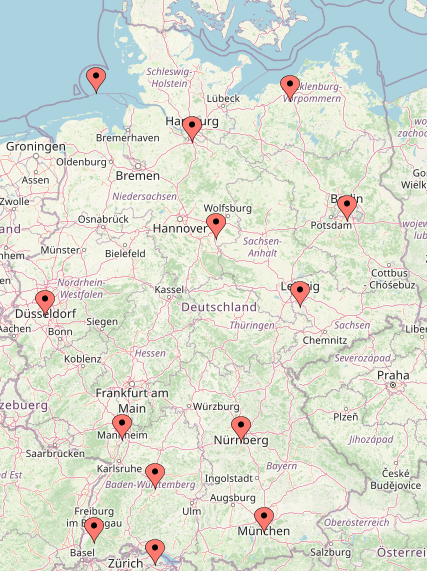
\includegraphics[width=.5\textwidth]{data/stations_map_customizer.png}
            \caption[Weather stations used]{Weather stations used}
            \label{fig::weather_stations}
 \end{figure}
 
\iffalse
\begin{table}[]
\centering
\begin{tabular}{l|l|l}
Station name & Measurements? & MOSMIX ?\\\hline
   Freiburg&Yes&Yes\\
   Hamburg&Yes&Yes\\
    Leipzig-Halle&Yes&Yes\\
    Nuernberg&Yes&Yes\\
    Stuttgart&Yes&Yes\\
    Mannheim&Yes&Yes\\
    Berlin-Tempelhof&Yes&Yes\\
    Duesseldorf&Yes&Yes\\
    Muenchen&Yes&Yes\\
   Konstanz&Yes&Yes\\
   Braunschweig&Yes&Yes\\
   Goettingen&Yes&Yes\\
   Rostock&Yes&Yes\\
   Helgoland&Yes&Yes   
\end{tabular}
\caption{Weather stations used for DWD data}
\label{Table::Weather_Stations}
\end{table}
\fi


 
 
% First explain concepts you used in your thesis like filters or methods
% Then explain your approach or algorithm
% Use flowcharts to give an overview

%\subsection{Additional Data}
%\label{Section::Additional_Data}
%On top of these 3 major thematic fields additional information about working days was used. 

%This data source is expected to capture variations in electricity load.
%School holidays and extended weekends due to public holidays are typical times for taking vacations.
%These effects will be analyzed later in the thesis.

%\subsubsection{Holidays}

%In germany there are static holidays which are always on the same day each year.
%Examples for these are christmas or the 1st of may. 
%Other holidays in germany are dependant on the date of easter. 
%An example for such a holiday is the feast of ascension, which always happens 39 days after easter.

%The bundesAPI provides an api to get information to get this information \cite{HolidayAPIUrl}.

%\subsubsection{School Holidays}

%Information about school holidays is provided by Schulferien.org \cite{SchoolHolidays}. 
%The data is displayed in a table on this website. 
%A webscraper is used to get the data.

\section{Evaluation metrics}
\label{Section:Evaluation_Metrics}

To evaluate the performance of the forecasting models, four metrics are used: two for deterministic accuracy and two for probabilistic forecast quality. This allows for a comprehensive assessment of both point forecasts and prediction intervals.

\subsection{Mean squared error (MSE) and Root Mean Squared Error (RMSE)}

The Mean Squared Error (MSE) and Root Mean Squared Error (RMSE) are used.
This metric is calculated using the formula $MSE = \frac{1}{n} \sum_{i=1}^{n}(Y_i - \hat{Y}_i)^2$
Due to the quadratic nature of this function large errors are penalized harder.

The RMSE is calculated using the formula $RMSE = \sqrt{MSE}$.
By taking the square root of the MSE the value for RMSE is in the same unit as the prediction values. 
This makes the RMSE easier to compare and interpret.

\subsection{Mean average error (MAE)}
The mean average error (MAE) is calculated using $MAE = \frac{1}{n} \sum_{i=1}^{n}|Y_i - \hat{Y}_i|$.
MAE measures the average magnitude of prediction errors, regardless of direction:
Unlike MSE, all deviations are treated equally.

This metric is in the same unit as the prediction values, making it easy to interpret.

\subsection{Continuous Ranked Probability Score (CRPS)}
CRPS evaluates the quality of probabilistic forecasts by comparing the predicted distribution to the actual outcome. In this thesis, it is approximated via pinball loss across a quantile grid: $CRPS = \frac{1}{R} \sum_{\tau\in r} PB_{\tau}$. 
This is calculated for a grid of probabilites $r$ between 0 and 1 of size $R$.
For the evaulation of the experiments $r=\{0.01, 0.02, ..., 0.99\}$ is used, resulting in $R=99$.

The formula for the pinball loss used to approximate the CRPS is $PB_{\tau} = (\tau - \mathbf{1}_{\{Y - \hat{Q}_{\tau}\}}) (Y-\hat{Q}_{\tau}) $,
where $\hat{Q}_{\tau}$ is a forecast of the $\tau -th$ quantile.

\subsection{$\tau$ \% coverage}
This metric measures the share of true values lying within a central prediction interval of width  $\tau$ .
The $\tau$ \% coverage is calculated by chosing a selecting a fraction for $\tau$ and inserting it into the formula $\tau\%-cov = \frac{1}{N} \sum_{i=1}^{N} \mathbf{1}_{\{\hat{Q}_{(1-\tau)/2} < Y_i < \hat{Q}_{(1+\tau)/2} \}}$
where $Y_i$ is the true value for datapoint $i$ and  $\hat{Q}_{\tau}$ is the $\tau -th$ quantile of all forecasts.

\section{Benchmark}
\label{Section:Benchmark}

In addition to comparing models against each other, this thesis uses the Intraday Index ID1 as a baseline benchmark. The ID1 reflects the volume-weighted average price of trades conducted on the intraday market up to one hour before delivery.

This index is used by market participants as a reference point for their final trading decisions and can be interpreted as a proxy for their implicit forecast of the imbalance price.

As explained in Section \ref{Section::Module_2} , the trades happening close to delivery time also play a formal role in Module 2 of the imbalance price calculation. In about 17\% of all settlement periods (2024), the imbalance price was directly influenced by the ID AEP value via the incentivizing component.

While the ID1 represents a strong and practical heuristic, it does not incorporate physical grid variables, weather uncertainty, or reserve activation data. Therefore, one objective of this thesis is to evaluate whether modern time series models can outperform this heuristic baseline under realistic forecasting conditions.


%During the experiments part of this thesis the models will be compared against each other.
%Another benchmark the models will be measured against is the intraday index ID1.
%The intraday index ID1 can be interpreted as a proxy for the market participants' forecast of the imbalance price.

%In a system that is short of energy, a trade for a price higher than the imbalance price would not make sense for a market participant fiscally.
%If no power is bought and instead balancing energy is used the imbalance price has to be paid. 
%As in this scenario the trade would cost more than receiving balancing energy, profit can be made by receiving balancing energy.

%As mentioned in section \ref{Section::Module_2} sometimes the imbalance price is set using the average price of the most recent prices.
%This incentive component was the price setting module only $17.23\%$ of the time in 2024.
%The most recent intraday price still is a very good and simple model \cite{narajewskiProbabilisticForecastingGerman2022}.


\end{document}
 		\clearpage
    \documentclass[class=scrbook, crop=false]{standalone}
\usepackage[subpreambles=true]{standalone}
\ifstandalone
    % WARNING: Proceed with caution!

% -----------------------------------------------------------------------------------
% For package standalone
% -----------------------------------------------------------------------------------
\usepackage{import}

% -----------------------------------------------------------------------------------
% Language and typeset
% -----------------------------------------------------------------------------------
\usepackage[ngerman, english]{babel}

\usepackage{subcaption}
% Umlauts and other special characters (UTF-8)
% \usepackage[utf8]{inputenc}
\usepackage{fontspec}
\setsansfont{Arial}
% \usepackage[T1]{fontenc}  % Enable accented characters and umlauts
% LuaLatex doesn't need fontenc and uses UTF-8
% \usepackage{lmodern}  % Font face


% --------------------------------------------------------------------------------
% Page formatting
% --------------------------------------------------------------------------------
% Change the header/footer for chapter beginnings and normal pages
\usepackage[automark,headsepline]{scrlayer-scrpage}

% The package provides an easy and flexible user interface to customize the page
% layout, implementing auto-centering and auto-balancing mechanisms
% WARNING: WHEN CHANGING BCOR (Binding correction), the cover needs reworking!...
\newcommand{\theBCOR}{15mm}  % Define binding correction
\usepackage[
    bindingoffset=\theBCOR,
    % showframe, % Show boxes which indicate margins and paddings
    bottom = 3.5cm, % Margins
      left = 2.5cm,
     right = 2.5cm
] {geometry}

% The package 'float' provides a container for document objects which can not be
% broken over pages, such as tables and figures
% Needed for table and figure indexes  
\usepackage{float}

% support for landscape layout
\usepackage{lscape}

% support of \tablenotes command to add notes under table
\usepackage{threeparttable}

% To allow drawing more professional tables
\usepackage{booktabs}

% --------------------------------------------------------------------------------
% Contents
% --------------------------------------------------------------------------------
% Vector graphics (for Cover page)
\usepackage{tikz} 

% Allows additional parameters when including images
\usepackage{graphicx}

% Roman font family for all headings
\addtokomafont{disposition}{\rmfamily}

% Set the line spacing to 1.5
\usepackage[onehalfspacing]{setspace}

% Improves overall text spacing
% http://www.khirevich.com/latex/microtype/
\usepackage[stretch=10]{microtype}

% Math symbols like mu outside the math environment
\usepackage{textcomp}

% A comprehensive (SI) units package∗
% For defining SI units
\usepackage[
    range-units=single,         % Formatting ranges with single unit indication: 1 - 2 m
    range-phrase=-,             % Phrase for range: 1 - 2 m vs 1 to 2 m
    separate-uncertainty=true,  % sets +- between value and uncertainty 
    multi-part-units=repeat     % In expressions with multiple values (multi part numbers) 
                                % the unit is printed each time: 1 mm x 1 mm
] {siunitx}
% https://tex.stackexchange.com/questions/124488/multi-part-numbers-and-units-in-siunitx

% Allows Sourcecodes with highlighting 
\usepackage{listings}

% This package provides user control over the layout of the three basic list
% environments: enumerate, itemize and description
\usepackage{enumitem}
\setlist{nosep} % Remove the vertical space between \item elements in all lists

% ToDo Notes
% \setlength{\marginparwidth}{2cm}
\usepackage{todonotes}
\setuptodonotes{inline, inlinepar}
\reversemarginpar  % Put ToDo notes on the binding's side
% \usepackage{soul} % Colorful ToDo notes

% Check out colors here http://latexcolor.com/
\usepackage{xcolor}

\usepackage{amsmath}    % alignment of equations

% --------------------------------------------------------------------------------
% Other elements
% --------------------------------------------------------------------------------
% Blindtext: Organic looking text dummy
\usepackage{blindtext}

% Hyperlinks within the document (PDF)
% "hidelinks" hides visual highlighting of links
\usepackage[hidelinks]{hyperref}

% Package for Glossary and Index (Acronyms are listed in a separate list) 
\usepackage[acronym, nogroupskip]{glossaries}[=v4.49] % groupskip: alphabetic grouping of entries

\usepackage{xltabular}   % <------- FOR glossaries

% Integration and management of bibliographies
\usepackage{csquotes}   % backend=biber in biblatex needs this package
\usepackage[
    style=ieee,   % style of the bibliography, entries are sorted in alphabetic order. "ieee" is another common style.
    backend=biber,      % based on package 'biber' 
    bibencoding=ascii   % ASCII Text encoding; may use "utf8" instead
] {biblatex}

% --------------------------------------------------------------------------------
%                               PATHS & FILES
% --------------------------------------------------------------------------------
% Fix paths for standalone compiling
\ifstandalone
    \def \home {..}
\else
    \def \home {.}
\fi

% Package: scrlayer-scrpage
% \def \stylePath {\home/settings+/style/page}
\input{\home/settings+/style/page}  % Load page style

% Package: graphicx
\graphicspath{{\home/images/}}  % Set path to images

% Package: listings
\input{\home/settings+/style/code.tex}  % Set path to style file
\lstset{inputpath={\home/code/}} % Default path to code listings

% Package: glossaries
\input{\home/settings+/style/symbols}  % Set path to symbols list style file
\input{\home/settings+/style/acronyms}  % Set path to acronym list style file
% -------------------------------------------------------------------------------
%               Listing of all Glossary and Acronym Entries 
%                           use as shown below
% -------------------------------------------------------------------------------

% ==== EXEMPLARY ENTRY FOR SYMBOLS LIST =========================================

% ==== EXEMPLARY ENTRY FOR ACRONYMS LIST ========================================
% \newacronym{#label}{#acronym}{#long_form}

% define new command for custom arconym entry with only two arguments
% fabricates an easier way to use \newacronym 
\newcommand{\acroX}[2]{\newacronym{#1}{#1}{#2}}
% \acroX{label and arconym}{long name}
% \acroX{CD}               {Compact Disk}

\newcommand{\acroY}[3]{\newacronym{#1}{#2}{#3}}
% \arcoY{label}{acronym}{long name}
% \acroY{CD}   {cd}     {Compact Disk}
 
\newacronym{AEP}{AEP}{Imbalance price}
\newacronym{aFRR}{aFRR}{Automatic Frequency Restoration Reserve}


\newacronym{reBAP}{reBAP}{Uniform imbalance price}
\newacronym{TSO}{TSO}{Transmission System Operator}
\newacronym{FCR}{FCR}{Frequency Containment Reserve}
\newacronym{mFRR}{mFRR}{Manual Frequency Restoration Reserve}
\newacronym{BRP}{BRP}{Balancing Responsible Party}
\newacronym{SB}{SB}{System Balance}
\newacronym{VRE}{VRE}{variable renewable energy}
\newacronym{ID1}{ID1}{intraday index ID1}
\newacronym{MAE}{MAE}{mean average error}
\newacronym{RMSE}{RMSE}{root mean squared error}
\newacronym{MSE}{MSE}{mean squared error}
\newacronym{CRPS}{CRPS}{continuous ranked probabililty score}
\newacronym{GCC}{GCC}{Grid Control Cooperation}
\newacronym{IC}{IC}{Continuous intraday}
\newacronym{VWAP}{VWAP}{volume-weighted average price}
\newacronym{VID}{VID}{traded volume within the intraday market}
\newacronym{ID AEP}{ID AEP}{Intraday Average Energy Price}
\newacronym{FRR}{FRR}{Frequency Restoration Reserve}
\newacronym{TFT}{TFT}{Temporal Fusion Transformer}
\newacronym{DLM}{DLM}{Dynamic Linear Model}
\newacronym{GB}{GB}{Gradient Boosting}
\newacronym{RF}{RF}{Random Forest}
\newacronym{ARIMAX}{ARIMAX}{Autoregressive Integrated Moving Average with eXogenous variables}
\newacronym{xLSTM}{xLSTM}{Extended Long Short-Term Memory}
\newacronym{DWD}{DWD}{Deutscher Wetterdienst}
\newacronym{ENTSO-E}{ENTSO-E}{European Network of Transmission System Operators for Electricity}
\newacronym{IDA1}{IDA1}{Intraday auction 1}
\newacronym{MOSMIX}{MOSMIX}{Model Output Statistics-MIX}
\newacronym{mLSTM}{mLSTM}{memory-optimized LSTM}
\newacronym{sLSTM}{sLSTM}{speed-optimized LSTM}

% ==== EXEMPLARY ENTRY FOR MAIN GLOSSARY ========================================

    % \newglossaryentry{policy}{name={Policy},description={Im geschäftlichen Bereich bezeichnet Policy eine interne Leit- bzw. Richtlinie, die formal durch das Unternehmen dokumentiert und über ihr Management verantwortet wird}}
    % \newglossaryentry{pcie}{name={PCI Express},description={PCI Express („Peripheral Component Interconnect Express“, abgekürzt PCIe oder PCI-E) ist ein Standard zur Verbindung von Peripheriegeräten mit dem Chipsatz eines Hauptprozessors. PCIe ist der Nachfolger von PCI, PCI-X und AGP und bietet im Vergleich zu seinen Vorgängern eine höhere Datenübertragungsrate pro Pin.}}
    % \newglossaryentry{realnumber}
  % Load glossary, symbol and acronyms list

% Package: biblatex
\addbibresource{\home/references/references.bib}  % Set path to bib resources

% Custom variables
\input{\home/settings+/variables}
% --------------------------------------------------------------------------------
%                                   OPTIONAL
% --------------------------------------------------------------------------------


% Simple arithmetic for LaTeX commands
% \usepackage{calc}

% Document Elements
% -------------------

% Index
% \usepackage{imakeidx}

% compact Lists
%\usepackage{paralist}

% visual improvements for citations
% \usepackage{epigraph}

% Create pseudo code
% https://www.overleaf.com/learn/latex/Algorithms
% \usepackage{algorithm}
% \usepackage{algorithmic}
%\usepackage[noend]{algpseudocode}

% Formatting
% -------------------
% Tweaks for scrbook, redefines commands of other packages
% \usepackage{scrhack}

% Intelligent space separator (nice for superscript?)
% \usepackage{xspace}

% Allows breaks within tables
%\usepackage{tabularx}

% Allows for page breaks in tables
% \usepackage{longtable}

% allows modifying of captions
% \usepackage{caption}

% Multiline comments
%\usepackage{verbatim}

% % Custom colors
% \definecolor{dartmouthgreen}{rgb}{0.05, 0.5, 0.06}

% IF you want to define unicode characters
% \DeclareUnicodeCharacter{0229}{\c{e}}
% \DeclareUnicodeCharacter{0306}{\u{Z}}


% Document elements
% ------------------------------------

% Table package
% \usepackage{booktabs}

% Pie diagram
% \usepackage{datapie}

% Side by Side images
% \usepackage{subcaption}

% For landscape tables
%\usepackage{pdflscape}
%\usepackage{afterpage}

% Graphics can be flow around by text
%\usepackage{wrapfig}

\fi
\usepackage[table]{xcolor}% http://ctan.org/pkg/xcolor

% ----------------------------------------------------------------------------
%                               Implementation
% ----------------------------------------------------------------------------
\begin{document}

\chapter{Implementation} % Outline text
\label{Chapter::Implementation}

% First explain concepts you used in your thesis like filters or methods
% Then explain your approach or algorithm
% Use flowcharts to give an overview
\section{Feature engineering}
\label{Section::Feature_engineering}
To improve predictive performance, the raw data introduced in Section \ref{Chapter::Data} is transformed into a set of engineered features. These features are designed to capture domain-specific relationships between the input variables and the imbalance price. Key transformations include the calculation of residual load and forecast errors.

Feature selection is guided by exploratory data analysis, domain knowledge, and statistical correlation with the target variable (\gls{reBAP}).


A normality check using the Anderson-Darling \cite{andersonAsymptoticTheoryCertain1952} test does not reject the assumption of normality, but due to the high skewness of $27.08$ and kurtosis of $1194.02$ normality can be rejected. Therefore, Spearman rank correlation is used to assess monotonic relationships between input features and the \gls{reBAP}.

\begin{figure}[H]
            \centering
            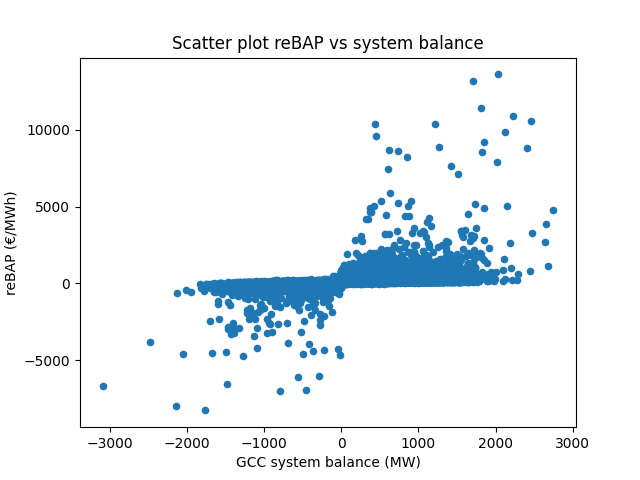
\includegraphics[width=.45\textwidth]{implementation/imbalance_scatter.pdf}
            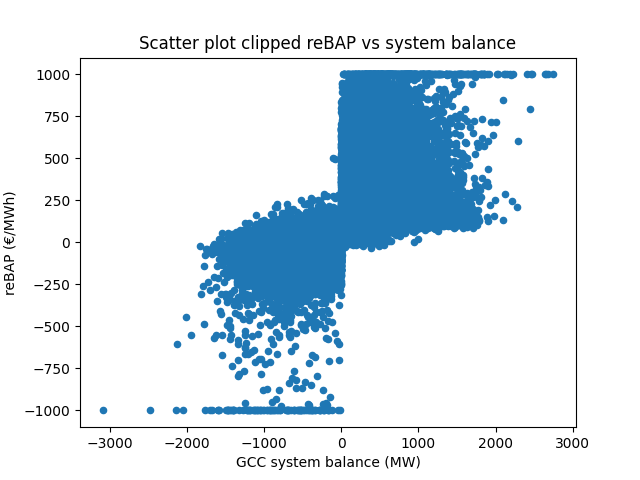
\includegraphics[width=.45\textwidth]{implementation/imbalance_scatter_clipped.pdf}
            \caption[Scatter plots for imbalance price and imbalance volume. For the plot on the right the imbalane price has been clipped to (-1000,1000) to give information about non-outliers]{Scatter plots for imbalance price and imbalance volume. For the plot on the right the imbalane price has been clipped to (-1000,1000) to give information about non-outliers}
            \label{Figure::volume_price_scatter}
\end{figure}

%The data introduced in section \ref{Chapter::Data} can be further refined to gain additional information. 
%The following sections contain information about how the data was used to create more features.
%Feature engineering was done for energy data, weather data and holiday data.

%In the following sections the correlation between features and the imbalance price will be explored.
%Using the anderson darling test \ref{andersonAsymptoticTheoryCertain1952} it was confirmed, that the data is normal distributed.
%A probability plot for the imbalance price can be seen in figure \ref{fig::rebap_distribution}. 
%The red line resembles a normal distribution. 
%The imbalance price has a skewness of $27.08$ and a kurtosis of $1194.02$, so the pearson correlation can not be used for analysing correlations.
%Instead for the following correlation analyses the spearman rank correlation will be used.

%\begin{figure}[ht]
%            \centering
 %           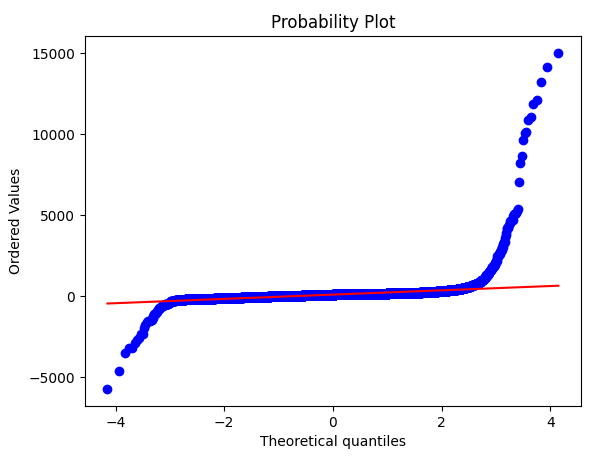
\includegraphics[width=.5\textwidth]{implementation/probability_plot.png}
%            \caption[Probability plot for the imbalance price]{Probability plot for the imbalance price}
%            \label{fig::rebap_distribution}
% \end{figure}


The imbalance volume and the imbalance price are highly correlated, having a correlation coefficient of $0.774$. 
Figure \ref{Figure::volume_price_scatter} shows scatter plots for the imbalance volume and imbalance price.
Due to the high correlation with the imbalance volume, correlations with the imbalance volumes will also be regarded for selecting new features.
The following sections describe the feature generation process for energy and weather data.


    \subsection{Energy data}
    \label{Section::FE_Energy_Data}

Several informative features are derived from the ENTSO-E dataset to capture dynamics relevant for the imbalance price. A central feature is the residual load, defined as the difference between total system load and the combined generation from wind (onshore and offshore) and solar:

Residual Load = Load−(Generation Wind\textsubscript{onshore} + Generation Wind\textsubscript{offshore} + Generation Solar)

This value reflects the part of the load that must be covered by dispatchable sources and is a key proxy for system stress.

Additionally, forecast errors are computed for load, generation, and residual load. These are calculated as the difference between forecasted and actual values for each variable. Since actual values are not available at prediction time, this feature is only available at the time the actual values are available. These features can also be used for analysis. 

    \begin{table}[h]
    \centering
    \begin{tabular}{l|l|l|l}
    Variable Name	&Forecasted Value& Actual Value	& Forecasting Error \\\hline
    Solar 		& -0.083		& -0.105		& \cellcolor{green} -0.155 \\
    Wind offshore 	& -0.164		& -0.152		& \cellcolor{green} 0.008 \\
    Wind onshore 	& -0.176		& \underline{-0.189}	& \cellcolor{green} -0.104 \\
    Load 		&0.101		& 0.121		& \cellcolor{green}  0.132 \\
    Residual Load 	& \cellcolor{green} \underline{0.343}& \cellcolor{green} \underline{0.391}& \cellcolor{green}0.192\\
    \end{tabular}

    
    \caption{Correlations between variables and \textbf{imbalance price} (rounded to next $10^{-3}$). Green cells are newly engineered features, the 3 most correlating features are underlined}
    \label{Table::Rebap_Correlations_ENTSOE}
    \end{table}

    \begin{table}[h]
    \centering
    \begin{tabular}{l|l|l|l}
    Variable Name	&Forecasted Value& Actual Value	& Forecasting Error \\\hline
    Solar 		&  -0.011		& -0.024		& \cellcolor{green} \underline{-0.149} \\
    Wind offshore 	& -0.013		&  -0.022		& \cellcolor{green}\underline{0.114}\\
    Wind onshore 	& 0.010		& 0.008		& \cellcolor{green} -0.093\\
    Load 		& 0.041		& 0.066		& \cellcolor{green}  -0.040 \\
    Residual Load 	& \cellcolor{green} 0.046& \cellcolor{green} 0.080& \cellcolor{green} \underline{0.193}\\
    \end{tabular}

    
    \caption{Correlations between variables and \textbf{imbalance volume} (rounded to next $10^{-3}$). Green cells are newly engineered features, the 3 most correlating features are underlined}
    \label{Table::Imbalance_volume_Correlations_ENTSOE}
    \end{table}

If other features that are available at prediction time correlate highly with the forecast errors, those features can be used to gain additional information.

Spearman rank correlation coefficients between the engineered features and the imbalance price are shown in Table \ref{Table::Rebap_Correlations_ENTSOE}. The strongest relationships are observed for residual load (actual and forecasted) as well as the forecast error of residual load.
Table \ref{Table::Imbalance_volume_Correlations_ENTSOE} presents the corresponding correlations with the imbalance volume. Here, the forecast errors also play a significant role, albeit with generally weaker correlations compared to the imbalance price.



   % The energy data provided by ENTSO-E can be further refined to gain additional information.
 %   One additional feature is the residual load. 
  %  Residual load is defined as the load that is not covered by VRE. 
%    This is calulated by subtracting the generation provided by solar, wind onshore and win offshore from the load.
    
   % Another way of generating more informative features is to calculate the forecasting error. 
%    For this the forecast for solar generation, wind generation and load is substracted from the actual measured values.
%    This can also be done for the residual load.
%   For each of these variables the correlation with the imbalance price is calclulated to estimate how much influence the variables have in determining the imbalance price.
 %   Table \ref{Table::Rebap_Correlations_ENTSOE} contains the results for these calculations. 
    
  %  Out of these features the forecasted and actual value for residual load and the residual load forecasting error correlate the most with the imbalance price.
 %   It should be noted that the actual values apart from the forecasts are not available at prediction time.    


%The correlation between the ENTSO-E data and the imbalance volume was calculated as well.
%The results for these calculations are displayd in table \ref{Table::Imbalance_volume_Correlations_ENTSOE}. The forecasted and actual value for the residual have a much lower correlation with the imbalance volume than with the imbalance price. The correlation between the residual load forecasting error and imbalance volume is about the same as with the imbalance price. Apart from the load the forecasting error correlates the most with the imbalance volume. 


    
    
    \subsection{Weather data}
    \label{Section::Weather_data}

The MOSMIX dataset from the \gls{DWD} provides high-resolution weather forecasts for up to 40 variables at hourly intervals. For each variable, forecasts are updated every hour and extend up to 10 days into the future.

To construct meaningful input features, two forecast timestamps are selected for each variable:
\begin{itemize}
\item the day-ahead forecast from 18:00 on the previous day 
\item the latest available forecast, typically issued two hours before gate closure
\end{itemize}
    
    \begin{table}[h]
    \centering
    \begin{tabular}{l|l}
    Variable Name	& Correlation coefficient \\\hline
   	LastFC\_FX1	&-0.254\\
	DayAhead\_FX1	&-0.25\\
	LastFC\_FF		&-0.247\\
	DayAhead\_FF 	&-0.243\\
	DayAhead\_N05	&0.185\\
	LastFC\_N05	&0.176\\
	DayAhead\_wwM	&0.167\\
	LastFC\_wwM	&0.162\\
	LastFC\_Rad1h 	&-0.128\\
	Diff\_Rad1h          	&-0.115\\
	LastFC\_SunD1     	&-0.102\\
    \end{tabular}
    
    \caption{Correlations between feature engineered MOSMIX variables and imbalance price with an absolute correlation coefficient larger than $0.1$ (rounded to next $10^{-3}$)}
    \label{Table::imbalance_price_MOSMIX_correlations}
    \end{table}
    
    \begin{table}[h]
    \centering
    \begin{tabular}{l|l}
    Variable Name	& Correlation coefficient \\\hline
	Diff\_Rad1h                          &-0.08\\
	LastFC\_N05                          &0.074\\
	DayAhead\_N05                        &0.073\\
	Diff\_TTT                           &-0.068\\
	Diff\_SunD1                         &-0.061\\
	Diff\_T5cm                          &-0.055\\
	Diff\_Nl                             &0.052\\
    \end{tabular}
    
    \caption{Correlations between feature engineered MOSMIX variables and imbalance volume (rounded to next $10^{-3}$)}
    \label{Table::imbalance_volume_MOSMIX_correlations}
    \end{table}
    
    
    \begin{table}[h]
    \centering
    \begin{tabular}{l|l}
    Variable Name	& Correlation coefficient \\\hline
	LastFC\_T5cm                        &-0.258\\
	DayAhead\_T5cm                      &-0.253\\
	LastFC\_TTT                         &-0.249\\
	DayAhead\_FF                         &0.246\\
	DayAhead\_TTT                       &-0.243\\
	LastFC\_FF                           &0.233\\
	LastFC\_Nl                           &0.221\\
	DayAhead\_FX1                        &0.216\\
	DayAhead\_Nl                         &0.205\\
	LastFC\_FX1                          &0.204\\
    \end{tabular}
    
    \caption{Correlations between feature engineered MOSMIX variables and residual load forecasting error with an absolute correlation coefficient larger than $0.2$ (rounded to next $10^{-3}$)}
    \label{Table::residual_load_fce_MOSMIX_correlations}
    \end{table}

The day-ahead forecast reflects what market participants may have relied on when submitting schedules, while the latest forecast provides the most accurate information available at prediction time.

In addition to using both forecast values directly, a third feature is calculated as the difference between the two forecasts, capturing the forecast revision and serving as a proxy for uncertainty.

Feature names are prefixed accordingly:
\begin{itemize}
\item DayAhead for the forecast of the day before
\item LastFC for the latest forecast
\item Diff  for the difference between the two
\end{itemize}
Spearman correlations between these features and the imbalance price, imbalance volume, and residual load forecasting error are reported in Tables \ref{Table::imbalance_price_MOSMIX_correlations},  \ref{Table::imbalance_volume_MOSMIX_correlations} and  \ref{Table::residual_load_fce_MOSMIX_correlations}.

The correlation with the residual load forecasting error was examined due to its observed correlation with both the reBAP and the imbalance volume. Since the MOSMIX features are available earlier than the actual residual load forecasting error, a strong correlation would allow earlier inference about future imbalance conditions.

Among the most relevant features are wind-related variables (FF, FX1), solar radiation (Rad1h, SunD1), and cloud cover (N05). These findings align with expectations, as VRE production and residual load strongly depend on weather dynamics.




    %The weather data contains a lot of datapoints, especially the MOSMIX forecast. 
  %  For each of the originally 40 features a forecast is done 240 times for each timestep. 
   % This data needs to be condensed, as not all of theses timestamps are useful.
   % There are certain timestamps which will be inspected closer for the feature engineering.
    
  %  The forecasts done by ENTSO-E are published the day before at 18:00. 
    %In the MOSMIX data this timestamp will be more closely looked at, because this is the latest forecast available for the forecast made by ENTSO-E.
    %Another important timestamp is the latest timestamp. This forecast has access to the most information, thus is most likely the most accurate forecast.
   % With a forecast being done each hour, the latest available timestamp at prediction time is the one 2 hours before gate closure time, due to the prediction happening at 1 hour before gate closure time.
   % For each of the MOSMIX variables the correlation for both of the previously discussed timestamps is checked.
    
  %  With both of these configurations for each of the variables a new feature can be created. 
   % To get an estimate for the forecasting error in the ENTSO-E data, the change in forecast can be calculated in the DWD data.
   % Under the assumption, that a more recent forecast is more accurate, the difference between the latest forecast and the forecast of the day before at $18:00$ is calculated.
   % The names for these new features are created by combining a prefix with the abbreviation for the MOSMIX feature.
  %  For the forecast from the previous day the prefix \textit{DayAhead} is used, the prefix \textit{LastFC} is used for the most recent forecast and \textit{Diff} denotes that the features is the difference between the day ahead forecast and the most recent forecast.
   % The results for the correlation analysis between the features and the imbalance can be found in table \ref{Table::imbalance_price_MOSMIX_correlations}. The results for the correlation analysis with the imbalance volume are displayed in table \ref{Table::imbalance_volume_MOSMIX_correlations}.
  %  The features containing information about wind, namely \textit{FX1} and \textit{FF}, show the highest correlation with the imbalance price. The parameter containing information about cloud coverage (\textit{N05}) is among the highest correlated with both the imbalance price and the imbalance volume. The same is true for the features containing information about solar radiation, \textit{Rad1h} and \textit{SunD1}. In general the correlation between the MOSMIX features and the imbalance volume are a lot lower than the correlations with the imbalance price.


\section{Data Split}
\label{Section::Data_Split}
To ensure a realistic evaluation of model performance, the dataset is chronologically split into three subsets:
\begin{itemize}
\item 70\% for training
\item 10\% for validation
\item 20\% for testing
\end{itemize}

The split is performed along the time axis to reflect real-world forecasting conditions and prevent data leakage between training and evaluation sets.

For Random Forest and \gls{ARIMAX}, the split can done by indexing the data. To ensure that these models have access to the same information as xLSTM and iTransformer, lagged featueres are introduced. For xLSTM and iTransformer, the data must be reshaped into time series sequences, and the split is performed explicitly on the full time-indexed dataset.

All models are evaluated on the same test period to ensure fair comparison. 

The forecast target is the reBAP one hour before energy delivery; hence, each model input only includes data available up to that point.


%To make sure the models trained during the experiments are comparable the models have to be trained and evaulated on the same dataset.
%The data was split into a set of training, validation and test data with a share of 70\%, 10\% and 20\% respectively.

%For random forest and arima this data split could be done using $train\_test\_split$ from the sklearn package. 
%With the more complex Time Series predictors xLSTM and iTransformer needing a different input shape this is a bit more complex.

%Instead the training, validation and test split was done along the temporal axis. 
%The oldest 70\% were defined as training data, the newest 20\% as test data, with the remaining 10\% being the validation data.


\section{Models}
\label{Section::Models}

Four forecasting models are used in this thesis, representing different modeling paradigms:
\begin{itemize}
\item Random Forest (ensemble learning)
\item ARIMAX (statistical time series modeling)
\item xLSTM (deep recurrent neural network)
\item iTransformer (inverted attention-based model)
\end{itemize}

The models differ in their ability to capture temporal dependencies and process structured input. Random Forest and ARIMAX require handcrafted lag features to encode time series behavior, while xLSTM and iTransformer directly process sequential data through specialized architectures.

For Random Forest, the RandomForestRegressor from scikit-learn is used, along with 4 lagged input versions for each feature (15min to 1h back). Hyperparameters are tuned using randomized search with 5-fold cross-validation, optimizing for RMSE.

For ARIMAX, the auto\_arima function from the pmdarima package is used. Only a subset of features is used as exogenous inputs due to computational constraints. Feature selection is based on the top 10 ranked variables from the Random Forest importance scores.

Both xLSTM and iTransformer require fixed-length input sequences. These are constructed using a sliding window approach with lookback lengths defined in the experiment setup (see Chapter \ref{Chapter::Experimental_Setup}). The deep learning models are implemented using PyTorch and trained on GPUs in the Google Cloud Vertex AI environment.

%In this section implementation details for each of the used models will be discussed. 
%The hyperparameter configurations might change during the experiments. 
%Any changes done specifically for an experiment will be discussed in the experiment's section.

%All the models were implemented in python. 
%
%\subsection{Random Forest}
%\label{Section::Random_Forest}

%As a random forest regressor the RandomForestRegressor provided by sklearn was used.
%Random forest can not use time series data out of the box.
%To give some more information about past timesteps shifted features are used.

%For the training in the experiments the timesteps of the previous 4 quarter hours were used.

%To find the best random forest regressor RandomizedSearchCV by sklearn was used.
%In total 20 different parameter combination were tested with a cross validation of 5.
%The performance of the models was measured using the negative mean squared error.

%\subsection{Arima}
%\label{Section::Arima}

%For the training of the arima model the module pmdarima was used.
%This module provides the function \textit{auto\_arima} to find the best arima model.
%The model was trained using the target variable as well as exogenous variables.
%The training time increases with the amount of exogenous variables.
%For that reason only a subset of features was used for this training.

%After the training of a random forest the importance of its features can be extracted using \textit{feature\_importances}. 
%The $10$ most important features were used for the training of the arima model.
%Using \textit{auto\_arima} the best parameter configuration can be found.

%\subsection{xLSTM}
%\label{Section::xLSTM}
%The configuration for the xLSTM models changes throughout the experiments and will be described in section \ref{Section::Experimental_Setup}

%\subsection{iTransformer}
%\label{Section::iTransformer}
%The configuration for the iTransformer models changes throughout the experiments and will be described in section \ref{Section::Experimental_Setup}



\end{document}
                                       \clearpage
    \documentclass[class=scrbook, crop=false]{standalone}
\usepackage[subpreambles=true]{standalone}
\ifstandalone
    % WARNING: Proceed with caution!

% -----------------------------------------------------------------------------------
% For package standalone
% -----------------------------------------------------------------------------------
\usepackage{import}

% -----------------------------------------------------------------------------------
% Language and typeset
% -----------------------------------------------------------------------------------
\usepackage[ngerman, english]{babel}

\usepackage{subcaption}
% Umlauts and other special characters (UTF-8)
% \usepackage[utf8]{inputenc}
\usepackage{fontspec}
\setsansfont{Arial}
% \usepackage[T1]{fontenc}  % Enable accented characters and umlauts
% LuaLatex doesn't need fontenc and uses UTF-8
% \usepackage{lmodern}  % Font face


% --------------------------------------------------------------------------------
% Page formatting
% --------------------------------------------------------------------------------
% Change the header/footer for chapter beginnings and normal pages
\usepackage[automark,headsepline]{scrlayer-scrpage}

% The package provides an easy and flexible user interface to customize the page
% layout, implementing auto-centering and auto-balancing mechanisms
% WARNING: WHEN CHANGING BCOR (Binding correction), the cover needs reworking!...
\newcommand{\theBCOR}{15mm}  % Define binding correction
\usepackage[
    bindingoffset=\theBCOR,
    % showframe, % Show boxes which indicate margins and paddings
    bottom = 3.5cm, % Margins
      left = 2.5cm,
     right = 2.5cm
] {geometry}

% The package 'float' provides a container for document objects which can not be
% broken over pages, such as tables and figures
% Needed for table and figure indexes  
\usepackage{float}

% support for landscape layout
\usepackage{lscape}

% support of \tablenotes command to add notes under table
\usepackage{threeparttable}

% To allow drawing more professional tables
\usepackage{booktabs}

% --------------------------------------------------------------------------------
% Contents
% --------------------------------------------------------------------------------
% Vector graphics (for Cover page)
\usepackage{tikz} 

% Allows additional parameters when including images
\usepackage{graphicx}

% Roman font family for all headings
\addtokomafont{disposition}{\rmfamily}

% Set the line spacing to 1.5
\usepackage[onehalfspacing]{setspace}

% Improves overall text spacing
% http://www.khirevich.com/latex/microtype/
\usepackage[stretch=10]{microtype}

% Math symbols like mu outside the math environment
\usepackage{textcomp}

% A comprehensive (SI) units package∗
% For defining SI units
\usepackage[
    range-units=single,         % Formatting ranges with single unit indication: 1 - 2 m
    range-phrase=-,             % Phrase for range: 1 - 2 m vs 1 to 2 m
    separate-uncertainty=true,  % sets +- between value and uncertainty 
    multi-part-units=repeat     % In expressions with multiple values (multi part numbers) 
                                % the unit is printed each time: 1 mm x 1 mm
] {siunitx}
% https://tex.stackexchange.com/questions/124488/multi-part-numbers-and-units-in-siunitx

% Allows Sourcecodes with highlighting 
\usepackage{listings}

% This package provides user control over the layout of the three basic list
% environments: enumerate, itemize and description
\usepackage{enumitem}
\setlist{nosep} % Remove the vertical space between \item elements in all lists

% ToDo Notes
% \setlength{\marginparwidth}{2cm}
\usepackage{todonotes}
\setuptodonotes{inline, inlinepar}
\reversemarginpar  % Put ToDo notes on the binding's side
% \usepackage{soul} % Colorful ToDo notes

% Check out colors here http://latexcolor.com/
\usepackage{xcolor}

\usepackage{amsmath}    % alignment of equations

% --------------------------------------------------------------------------------
% Other elements
% --------------------------------------------------------------------------------
% Blindtext: Organic looking text dummy
\usepackage{blindtext}

% Hyperlinks within the document (PDF)
% "hidelinks" hides visual highlighting of links
\usepackage[hidelinks]{hyperref}

% Package for Glossary and Index (Acronyms are listed in a separate list) 
\usepackage[acronym, nogroupskip]{glossaries}[=v4.49] % groupskip: alphabetic grouping of entries

\usepackage{xltabular}   % <------- FOR glossaries

% Integration and management of bibliographies
\usepackage{csquotes}   % backend=biber in biblatex needs this package
\usepackage[
    style=ieee,   % style of the bibliography, entries are sorted in alphabetic order. "ieee" is another common style.
    backend=biber,      % based on package 'biber' 
    bibencoding=ascii   % ASCII Text encoding; may use "utf8" instead
] {biblatex}

% --------------------------------------------------------------------------------
%                               PATHS & FILES
% --------------------------------------------------------------------------------
% Fix paths for standalone compiling
\ifstandalone
    \def \home {..}
\else
    \def \home {.}
\fi

% Package: scrlayer-scrpage
% \def \stylePath {\home/settings+/style/page}
\input{\home/settings+/style/page}  % Load page style

% Package: graphicx
\graphicspath{{\home/images/}}  % Set path to images

% Package: listings
\input{\home/settings+/style/code.tex}  % Set path to style file
\lstset{inputpath={\home/code/}} % Default path to code listings

% Package: glossaries
\input{\home/settings+/style/symbols}  % Set path to symbols list style file
\input{\home/settings+/style/acronyms}  % Set path to acronym list style file
% -------------------------------------------------------------------------------
%               Listing of all Glossary and Acronym Entries 
%                           use as shown below
% -------------------------------------------------------------------------------

% ==== EXEMPLARY ENTRY FOR SYMBOLS LIST =========================================

% ==== EXEMPLARY ENTRY FOR ACRONYMS LIST ========================================
% \newacronym{#label}{#acronym}{#long_form}

% define new command for custom arconym entry with only two arguments
% fabricates an easier way to use \newacronym 
\newcommand{\acroX}[2]{\newacronym{#1}{#1}{#2}}
% \acroX{label and arconym}{long name}
% \acroX{CD}               {Compact Disk}

\newcommand{\acroY}[3]{\newacronym{#1}{#2}{#3}}
% \arcoY{label}{acronym}{long name}
% \acroY{CD}   {cd}     {Compact Disk}
 
\newacronym{AEP}{AEP}{Imbalance price}
\newacronym{aFRR}{aFRR}{Automatic Frequency Restoration Reserve}


\newacronym{reBAP}{reBAP}{Uniform imbalance price}
\newacronym{TSO}{TSO}{Transmission System Operator}
\newacronym{FCR}{FCR}{Frequency Containment Reserve}
\newacronym{mFRR}{mFRR}{Manual Frequency Restoration Reserve}
\newacronym{BRP}{BRP}{Balancing Responsible Party}
\newacronym{SB}{SB}{System Balance}
\newacronym{VRE}{VRE}{variable renewable energy}
\newacronym{ID1}{ID1}{intraday index ID1}
\newacronym{MAE}{MAE}{mean average error}
\newacronym{RMSE}{RMSE}{root mean squared error}
\newacronym{MSE}{MSE}{mean squared error}
\newacronym{CRPS}{CRPS}{continuous ranked probabililty score}
\newacronym{GCC}{GCC}{Grid Control Cooperation}
\newacronym{IC}{IC}{Continuous intraday}
\newacronym{VWAP}{VWAP}{volume-weighted average price}
\newacronym{VID}{VID}{traded volume within the intraday market}
\newacronym{ID AEP}{ID AEP}{Intraday Average Energy Price}
\newacronym{FRR}{FRR}{Frequency Restoration Reserve}
\newacronym{TFT}{TFT}{Temporal Fusion Transformer}
\newacronym{DLM}{DLM}{Dynamic Linear Model}
\newacronym{GB}{GB}{Gradient Boosting}
\newacronym{RF}{RF}{Random Forest}
\newacronym{ARIMAX}{ARIMAX}{Autoregressive Integrated Moving Average with eXogenous variables}
\newacronym{xLSTM}{xLSTM}{Extended Long Short-Term Memory}
\newacronym{DWD}{DWD}{Deutscher Wetterdienst}
\newacronym{ENTSO-E}{ENTSO-E}{European Network of Transmission System Operators for Electricity}
\newacronym{IDA1}{IDA1}{Intraday auction 1}
\newacronym{MOSMIX}{MOSMIX}{Model Output Statistics-MIX}
\newacronym{mLSTM}{mLSTM}{memory-optimized LSTM}
\newacronym{sLSTM}{sLSTM}{speed-optimized LSTM}

% ==== EXEMPLARY ENTRY FOR MAIN GLOSSARY ========================================

    % \newglossaryentry{policy}{name={Policy},description={Im geschäftlichen Bereich bezeichnet Policy eine interne Leit- bzw. Richtlinie, die formal durch das Unternehmen dokumentiert und über ihr Management verantwortet wird}}
    % \newglossaryentry{pcie}{name={PCI Express},description={PCI Express („Peripheral Component Interconnect Express“, abgekürzt PCIe oder PCI-E) ist ein Standard zur Verbindung von Peripheriegeräten mit dem Chipsatz eines Hauptprozessors. PCIe ist der Nachfolger von PCI, PCI-X und AGP und bietet im Vergleich zu seinen Vorgängern eine höhere Datenübertragungsrate pro Pin.}}
    % \newglossaryentry{realnumber}
  % Load glossary, symbol and acronyms list

% Package: biblatex
\addbibresource{\home/references/references.bib}  % Set path to bib resources

% Custom variables
\input{\home/settings+/variables}
% --------------------------------------------------------------------------------
%                                   OPTIONAL
% --------------------------------------------------------------------------------


% Simple arithmetic for LaTeX commands
% \usepackage{calc}

% Document Elements
% -------------------

% Index
% \usepackage{imakeidx}

% compact Lists
%\usepackage{paralist}

% visual improvements for citations
% \usepackage{epigraph}

% Create pseudo code
% https://www.overleaf.com/learn/latex/Algorithms
% \usepackage{algorithm}
% \usepackage{algorithmic}
%\usepackage[noend]{algpseudocode}

% Formatting
% -------------------
% Tweaks for scrbook, redefines commands of other packages
% \usepackage{scrhack}

% Intelligent space separator (nice for superscript?)
% \usepackage{xspace}

% Allows breaks within tables
%\usepackage{tabularx}

% Allows for page breaks in tables
% \usepackage{longtable}

% allows modifying of captions
% \usepackage{caption}

% Multiline comments
%\usepackage{verbatim}

% % Custom colors
% \definecolor{dartmouthgreen}{rgb}{0.05, 0.5, 0.06}

% IF you want to define unicode characters
% \DeclareUnicodeCharacter{0229}{\c{e}}
% \DeclareUnicodeCharacter{0306}{\u{Z}}


% Document elements
% ------------------------------------

% Table package
% \usepackage{booktabs}

% Pie diagram
% \usepackage{datapie}

% Side by Side images
% \usepackage{subcaption}

% For landscape tables
%\usepackage{pdflscape}
%\usepackage{afterpage}

% Graphics can be flow around by text
%\usepackage{wrapfig}

\fi

% ----------------------------------------------------------------------------
%                               Results
% ----------------------------------------------------------------------------
\begin{document}

\chapter{Experimental Setup} % Overview text
\label{Chapter::Experimental_Setup}
   This chapter contains information about the configurations and models used for each experiment. 
   For each experiment different approaches were tried to improve the model performance.

% Explain the setup of your experiment in such a way that others could repeat it
% First, explain the environment of the experiment
% Second, explain the tools used
% Lastly, how is everything setup for the experiment, what are the variables?
% Do not discuss results here !!!
\section{Experiment: Out of the box performance}
\label{Section::Experiment_out_of_the_box}

In this experiment different Time Series predictors are compared against each other.
The models used for this are naive, random forest, arima, iTransformer and xLSTM.
The naive model is a benchmark that predicts the imbalance price to be the intraday index ID1. 

For random forest and arima some additional lagged features are created to give information about the data being time series data.
For each feature lagged features are introduced, the features are lagged by 15 minutes, 30 minutes, 45 minutes and an hour.
Also weekly lagged features are used. 
The features are lagged by one and by two weeks.

For the iTransformer model and xLSTM model the hyperparameter configuration can be found in table \ref{Table::Raw_hyperparameters}.
The hyperparameter configurations are the same across all experiments unless specified differently.
The xLSTM block configuration used for this experiment was $xlstm\_7\_1$. 
The numbers in $xlstm\_i\_k$ represent the amount of mLSTM vs sLSTM cells used in the xLSTM block.
This configuration uses 7 times as many mLSTM blocks than sLSTM blocks. 
In total 48 blocks are used. 

\begin{table}[]
\centering
\begin{tabular}{l|l|l}
 Hyperparameter name & iTransformer & xLSTM   \\\hline
 Learning rate & $10^{-3}$ & $10^{-3} $ \\
 Sequence length & 96 & 96  \\
 Batch size & 16 & 32  \\
 Embedding dimension & 512 & 128  \\
 
\end{tabular}
\caption{Hyperparameter configuration for iTransformer and xLSTM}
\label{Table::Raw_hyperparameters}
\end{table}

\section{Experiment: xLSTM different xLSTM block structures}
In this experiment different xLSTM configurations were compared. 
The goal was to check whether it would suffice to only use mLSTM or sLSTM cells compared to the model used in the previous experiment.
Three different xLSTM models were trained and their results compared.
Each model contains an xLSTM block with 48 modules.
The different models are named xlstm\_n\_m, where n:m denotes the fraction of mLSTM to sLSTM blocks.
The configurations tested were xlstm\_1\_0, xlstm\_7\_1 and xlstm\_0\_1. 

  \begin{table}[]
\centering
\begin{tabular}{l|l}
 Configuration name & Amount of mLSTM blocks & Amount of sLSTM blocks  \\\hline
 xlstm\_1\_0 & 48 & 0 \\
 xlstm\_0\_1 & 0 & 48 \\
 xlstm\_7\_1  & 42 & 6 
\end{tabular}
\caption{xLSTM Configurations}
\label{Table::xLSTM_configuratiosn}
\end{table}

\section{Experiment: iTransformer variable sequence length}
   
   In this experiment iTransformer models were trained to inspect how sequence length changes model performance.
   The idea behind this experiment was to check whether more information about the past improves the prediction.
   For this the sequence lengths 96, 192 and 384 were used. Other than that the hyperparameters were the same as shown in table \ref{Table::Raw_hyperparameters}   
   
\section{Experiment: iTransformer multiple target variables}

  In this experiment the iTransformer model was trained on multiple target variables.
  The goal of this experiment was to check whether learning to predict other variables would improve the performance.
  This kind of training should encourage the model to learn a better general understanding of the data instead of just predicting the imbalance price.
  During the training the loss is calculated on all of the target variables. 
  During the testing only the prediction for imbalance price is used to calculate the error metrics.
  A list with the target variables for each configuration can be found in table \ref{Table::Multiple_targets}, the other hyperparameters are not changed from \ref{Table::Raw_hyperparameters}.
  
  \begin{table}[]
\centering
\begin{tabular}{l|l}
 Configuration name & Target variables  \\\hline
 Intraday indices&   Intraday index IDFULL\\
 		& Intraday index ID1 \\
 		& Intraday index ID3 \\ \hline
 Entsoe data & Actual fossil gas generation  \\
 		& Actual fossil hard coal generation \\
 		& Actual lignite generation \\ \hline
 Netzregelverbund & Imbalance volume  \\
 		& Activated primary balancing capacity \\
 		& Activated secondary balancing capacity \\ \hline
 Combined & Imbalance volume   \\
 		& Intraday index IDFULL \\
 		& Actual fossil hard coal generation \\ 
\end{tabular}
\caption{Configurations for multiple target variables}
\label{Table::Multiple_Targets}
\end{table}

\section{Experiment: iTransformer longer forecast horizon}

In this experiment it was checked, whether a longer forecast horizon would increase the performance of the time series predictor.
During training and validation losses on the complete forecast horizon were used.
During testing only  the forecast which was forecast in the other experiments was used to calculate the evaluation metrics.

The goal behind this experiment was to check whether the model would benefit from trying to learn a longer trend than just a single point in time.
For this different horizons were compared. The horizon starts at the prediction timestamp, so an hour from the prediction time.
The horizons used during this experiments are 4, which corresponds to an hour, 48, which corresponds to half of a day and 96, which corresponds to a full day.
\end{document}
                                           \clearpage
    \documentclass[class=scrbook, crop=false]{standalone}
\usepackage[subpreambles=true]{standalone}
\ifstandalone
    % WARNING: Proceed with caution!

% -----------------------------------------------------------------------------------
% For package standalone
% -----------------------------------------------------------------------------------
\usepackage{import}

% -----------------------------------------------------------------------------------
% Language and typeset
% -----------------------------------------------------------------------------------
\usepackage[ngerman, english]{babel}

\usepackage{subcaption}
% Umlauts and other special characters (UTF-8)
% \usepackage[utf8]{inputenc}
\usepackage{fontspec}
\setsansfont{Arial}
% \usepackage[T1]{fontenc}  % Enable accented characters and umlauts
% LuaLatex doesn't need fontenc and uses UTF-8
% \usepackage{lmodern}  % Font face


% --------------------------------------------------------------------------------
% Page formatting
% --------------------------------------------------------------------------------
% Change the header/footer for chapter beginnings and normal pages
\usepackage[automark,headsepline]{scrlayer-scrpage}

% The package provides an easy and flexible user interface to customize the page
% layout, implementing auto-centering and auto-balancing mechanisms
% WARNING: WHEN CHANGING BCOR (Binding correction), the cover needs reworking!...
\newcommand{\theBCOR}{15mm}  % Define binding correction
\usepackage[
    bindingoffset=\theBCOR,
    % showframe, % Show boxes which indicate margins and paddings
    bottom = 3.5cm, % Margins
      left = 2.5cm,
     right = 2.5cm
] {geometry}

% The package 'float' provides a container for document objects which can not be
% broken over pages, such as tables and figures
% Needed for table and figure indexes  
\usepackage{float}

% support for landscape layout
\usepackage{lscape}

% support of \tablenotes command to add notes under table
\usepackage{threeparttable}

% To allow drawing more professional tables
\usepackage{booktabs}

% --------------------------------------------------------------------------------
% Contents
% --------------------------------------------------------------------------------
% Vector graphics (for Cover page)
\usepackage{tikz} 

% Allows additional parameters when including images
\usepackage{graphicx}

% Roman font family for all headings
\addtokomafont{disposition}{\rmfamily}

% Set the line spacing to 1.5
\usepackage[onehalfspacing]{setspace}

% Improves overall text spacing
% http://www.khirevich.com/latex/microtype/
\usepackage[stretch=10]{microtype}

% Math symbols like mu outside the math environment
\usepackage{textcomp}

% A comprehensive (SI) units package∗
% For defining SI units
\usepackage[
    range-units=single,         % Formatting ranges with single unit indication: 1 - 2 m
    range-phrase=-,             % Phrase for range: 1 - 2 m vs 1 to 2 m
    separate-uncertainty=true,  % sets +- between value and uncertainty 
    multi-part-units=repeat     % In expressions with multiple values (multi part numbers) 
                                % the unit is printed each time: 1 mm x 1 mm
] {siunitx}
% https://tex.stackexchange.com/questions/124488/multi-part-numbers-and-units-in-siunitx

% Allows Sourcecodes with highlighting 
\usepackage{listings}

% This package provides user control over the layout of the three basic list
% environments: enumerate, itemize and description
\usepackage{enumitem}
\setlist{nosep} % Remove the vertical space between \item elements in all lists

% ToDo Notes
% \setlength{\marginparwidth}{2cm}
\usepackage{todonotes}
\setuptodonotes{inline, inlinepar}
\reversemarginpar  % Put ToDo notes on the binding's side
% \usepackage{soul} % Colorful ToDo notes

% Check out colors here http://latexcolor.com/
\usepackage{xcolor}

\usepackage{amsmath}    % alignment of equations

% --------------------------------------------------------------------------------
% Other elements
% --------------------------------------------------------------------------------
% Blindtext: Organic looking text dummy
\usepackage{blindtext}

% Hyperlinks within the document (PDF)
% "hidelinks" hides visual highlighting of links
\usepackage[hidelinks]{hyperref}

% Package for Glossary and Index (Acronyms are listed in a separate list) 
\usepackage[acronym, nogroupskip]{glossaries}[=v4.49] % groupskip: alphabetic grouping of entries

\usepackage{xltabular}   % <------- FOR glossaries

% Integration and management of bibliographies
\usepackage{csquotes}   % backend=biber in biblatex needs this package
\usepackage[
    style=ieee,   % style of the bibliography, entries are sorted in alphabetic order. "ieee" is another common style.
    backend=biber,      % based on package 'biber' 
    bibencoding=ascii   % ASCII Text encoding; may use "utf8" instead
] {biblatex}

% --------------------------------------------------------------------------------
%                               PATHS & FILES
% --------------------------------------------------------------------------------
% Fix paths for standalone compiling
\ifstandalone
    \def \home {..}
\else
    \def \home {.}
\fi

% Package: scrlayer-scrpage
% \def \stylePath {\home/settings+/style/page}
\input{\home/settings+/style/page}  % Load page style

% Package: graphicx
\graphicspath{{\home/images/}}  % Set path to images

% Package: listings
\input{\home/settings+/style/code.tex}  % Set path to style file
\lstset{inputpath={\home/code/}} % Default path to code listings

% Package: glossaries
\input{\home/settings+/style/symbols}  % Set path to symbols list style file
\input{\home/settings+/style/acronyms}  % Set path to acronym list style file
% -------------------------------------------------------------------------------
%               Listing of all Glossary and Acronym Entries 
%                           use as shown below
% -------------------------------------------------------------------------------

% ==== EXEMPLARY ENTRY FOR SYMBOLS LIST =========================================

% ==== EXEMPLARY ENTRY FOR ACRONYMS LIST ========================================
% \newacronym{#label}{#acronym}{#long_form}

% define new command for custom arconym entry with only two arguments
% fabricates an easier way to use \newacronym 
\newcommand{\acroX}[2]{\newacronym{#1}{#1}{#2}}
% \acroX{label and arconym}{long name}
% \acroX{CD}               {Compact Disk}

\newcommand{\acroY}[3]{\newacronym{#1}{#2}{#3}}
% \arcoY{label}{acronym}{long name}
% \acroY{CD}   {cd}     {Compact Disk}
 
\newacronym{AEP}{AEP}{Imbalance price}
\newacronym{aFRR}{aFRR}{Automatic Frequency Restoration Reserve}


\newacronym{reBAP}{reBAP}{Uniform imbalance price}
\newacronym{TSO}{TSO}{Transmission System Operator}
\newacronym{FCR}{FCR}{Frequency Containment Reserve}
\newacronym{mFRR}{mFRR}{Manual Frequency Restoration Reserve}
\newacronym{BRP}{BRP}{Balancing Responsible Party}
\newacronym{SB}{SB}{System Balance}
\newacronym{VRE}{VRE}{variable renewable energy}
\newacronym{ID1}{ID1}{intraday index ID1}
\newacronym{MAE}{MAE}{mean average error}
\newacronym{RMSE}{RMSE}{root mean squared error}
\newacronym{MSE}{MSE}{mean squared error}
\newacronym{CRPS}{CRPS}{continuous ranked probabililty score}
\newacronym{GCC}{GCC}{Grid Control Cooperation}
\newacronym{IC}{IC}{Continuous intraday}
\newacronym{VWAP}{VWAP}{volume-weighted average price}
\newacronym{VID}{VID}{traded volume within the intraday market}
\newacronym{ID AEP}{ID AEP}{Intraday Average Energy Price}
\newacronym{FRR}{FRR}{Frequency Restoration Reserve}
\newacronym{TFT}{TFT}{Temporal Fusion Transformer}
\newacronym{DLM}{DLM}{Dynamic Linear Model}
\newacronym{GB}{GB}{Gradient Boosting}
\newacronym{RF}{RF}{Random Forest}
\newacronym{ARIMAX}{ARIMAX}{Autoregressive Integrated Moving Average with eXogenous variables}
\newacronym{xLSTM}{xLSTM}{Extended Long Short-Term Memory}
\newacronym{DWD}{DWD}{Deutscher Wetterdienst}
\newacronym{ENTSO-E}{ENTSO-E}{European Network of Transmission System Operators for Electricity}
\newacronym{IDA1}{IDA1}{Intraday auction 1}
\newacronym{MOSMIX}{MOSMIX}{Model Output Statistics-MIX}
\newacronym{mLSTM}{mLSTM}{memory-optimized LSTM}
\newacronym{sLSTM}{sLSTM}{speed-optimized LSTM}

% ==== EXEMPLARY ENTRY FOR MAIN GLOSSARY ========================================

    % \newglossaryentry{policy}{name={Policy},description={Im geschäftlichen Bereich bezeichnet Policy eine interne Leit- bzw. Richtlinie, die formal durch das Unternehmen dokumentiert und über ihr Management verantwortet wird}}
    % \newglossaryentry{pcie}{name={PCI Express},description={PCI Express („Peripheral Component Interconnect Express“, abgekürzt PCIe oder PCI-E) ist ein Standard zur Verbindung von Peripheriegeräten mit dem Chipsatz eines Hauptprozessors. PCIe ist der Nachfolger von PCI, PCI-X und AGP und bietet im Vergleich zu seinen Vorgängern eine höhere Datenübertragungsrate pro Pin.}}
    % \newglossaryentry{realnumber}
  % Load glossary, symbol and acronyms list

% Package: biblatex
\addbibresource{\home/references/references.bib}  % Set path to bib resources

% Custom variables
\input{\home/settings+/variables}
% --------------------------------------------------------------------------------
%                                   OPTIONAL
% --------------------------------------------------------------------------------


% Simple arithmetic for LaTeX commands
% \usepackage{calc}

% Document Elements
% -------------------

% Index
% \usepackage{imakeidx}

% compact Lists
%\usepackage{paralist}

% visual improvements for citations
% \usepackage{epigraph}

% Create pseudo code
% https://www.overleaf.com/learn/latex/Algorithms
% \usepackage{algorithm}
% \usepackage{algorithmic}
%\usepackage[noend]{algpseudocode}

% Formatting
% -------------------
% Tweaks for scrbook, redefines commands of other packages
% \usepackage{scrhack}

% Intelligent space separator (nice for superscript?)
% \usepackage{xspace}

% Allows breaks within tables
%\usepackage{tabularx}

% Allows for page breaks in tables
% \usepackage{longtable}

% allows modifying of captions
% \usepackage{caption}

% Multiline comments
%\usepackage{verbatim}

% % Custom colors
% \definecolor{dartmouthgreen}{rgb}{0.05, 0.5, 0.06}

% IF you want to define unicode characters
% \DeclareUnicodeCharacter{0229}{\c{e}}
% \DeclareUnicodeCharacter{0306}{\u{Z}}


% Document elements
% ------------------------------------

% Table package
% \usepackage{booktabs}

% Pie diagram
% \usepackage{datapie}

% Side by Side images
% \usepackage{subcaption}

% For landscape tables
%\usepackage{pdflscape}
%\usepackage{afterpage}

% Graphics can be flow around by text
%\usepackage{wrapfig}

\fi

% ----------------------------------------------------------------------------
%                               Discussion
% ----------------------------------------------------------------------------
\begin{document}

\chapter{Results and Discussion} % Overview text
\label{Chapter::Results and Discussion}
In this chapter, the results of the thesis are discussed. The following sections contain th results of the experiments specified in \ref{Chapter::Experiments}.                   
    In this chapter, the results of the thesis are presented and evaluated as well as, the approach of this thesis.

% Show your results and analyze them
% Explain why the results are the way they are and not different
% Go into possible measurement errors and why they occurred
% Look for anomalies and explain why they occur
\section{Results}
\label{Section::Results}

\section{Out of the box performance}

The comparison of out-of-the-box model performance (Tables \ref{Table::Out_of_the_box_performance} and \ref{Table::Out_of_the_box_performance_quantile}) highlights clear differences in how each approach handles point forecasting, probabilistic estimation, and tail risk.

The xLSTM model achieves the strongest overall performance, with the lowest MAE (84.33), outperforming the naive ID1, and lowest CRPS (40.30) across all models. It also performs competitively in RMSE (302.57), suggesting that it not only captures average-case dynamics reliably, but also handles larger deviations effectively.

The iTransformer, by contrast, achieves the lowest RMSE (200.19), suggesting strong sensitivity to extreme price events. However, it exhibits the highest MAE (139.87) and CRPS (49.24), which points to less stable average-case performance and weaker calibration. Notably, its coverage rates are the highest across all models (e.g. 98\%-coverage of 0.959).

The Random Forest model provides solid baseline performance, with a relatively low MAE (99.00) and the second-best CRPS (41.37). Its RMSE (353.81) is notably higher, indicating reduced robustness to extreme values. Nevertheless, its prediction intervals are among the most reliable in the mid quantiles, with strong 90\%- and 98\%-coverage.

The ARIMA model performs similarly to Random Forest in terms of MAE (100.50) and CRPS (42.04), but has the highest RMSE (358.75) among all models, suggesting that it fails to capture large price spikes — a known limitation of linear, autoregressive models.

As shown in Figure \ref{Figure::pinball_scores}, the iTransformer achieves the lowest normalized pinball loss at the 90th percentile, highlighting their strength in forecasting extreme imbalance price events. This suggests that this model is well-suited to anticipating high-price outliers, which aligns with their superior RMSE compared to the other models.
In contrast, Random Forest, ARIMA and xLSTM perform better in the lower and mid quantiles, aligning with their lower MAE and CRPS. These models offer more accurate average-case predictions, but struggle with extreme events, which limits their effectiveness in capturing tail risk.

Compared to the naive ID1 benchmark, the trained models show mixed performance. While Random Forest, ARIMA and xLSTM outperform ID1 in CRPS, and iTransformer in RMSE, only xLSTM achieves a lower MAE than ID1.
However, when it comes to prediction interval coverage, all models surpass the benchmark significantly, with iTransformer achieving the best 50\%, 90\%, and 98\% coverage among all models.

These results support the thesis hypothesis: modern deep learning models can outperform classical methods and naive market heuristics, particularly for tail risks. However, Random Forest proves highly competitive—offering robust performance without the need for extensive tuning or sequence modeling.


  
  \begin{table}[]
\centering
\begin{tabular}{l|l|l|l}
Model name 		&  RMSE 			& MAE 			& CRPS 			\\\hline
Naive intraday ID1 	&$ 308.69 			$&$ 93.17 			$&$ 42.90			$ \\
Random forest 		&$ 353.81 \pm 0.19	$&$  99.00	\pm 0.17	$&$ 41.37 \pm 0.06	$\\
Arima 			&$ 358.75 			$&$ 100.50 		$&$ 42.04  			$\\	
iTransformer 		&$ \underline{200.19 \pm 0.07}	$&$ 139.87	\pm 0.06	$&$ 49.24 \pm 0.04	$ \\
xLSTM 			&$ 302.57\pm 6.68	$&$ \underline{84.33 \pm 1.17}	$&$ \underline{40.30	\pm0.24} $\\
\end{tabular}
\caption{Error metrics and CRPS for out of the box performance}
\label{Table::Out_of_the_box_performance}
\end{table}
\begin{table}
\centering
\begin{tabular}{l|l|l|l}
Model name 		&  50\%-cov 		& 90\%-cov 		& 98\%-cov \\\hline
Naive intraday ID1 	&$ 0.084			$&$ 0.557 			$&$ 0.844			$ \\
Random forest 		&$ 0.147 \pm0.003	$&$ 0.772\pm 0.007	$&$ 0.945	 \pm 0.005	$\\
Arima 			&$ 0.211			$&$ 0.612	 		$&$0.810 			$\\	
iTransformer 		&$ \underline{0.356	\pm 0.001}	$&$ \underline{0.841	\pm 0.000}	$&$ \underline{0.959 \pm 0.000}	$ \\
xLSTM 			&$ 0.240 \pm 0.019	$&$ 0.759 	\pm 0.012	$&$ 0.910 \pm 0.009	 $\\
\end{tabular}
\caption{Quantile metrics for out of the box performance}
\label{Table::Out_of_the_box_performance_quantile}
\end{table}


\begin{figure}
  \centering
\begin{subfigure}{0.45\textwidth}
  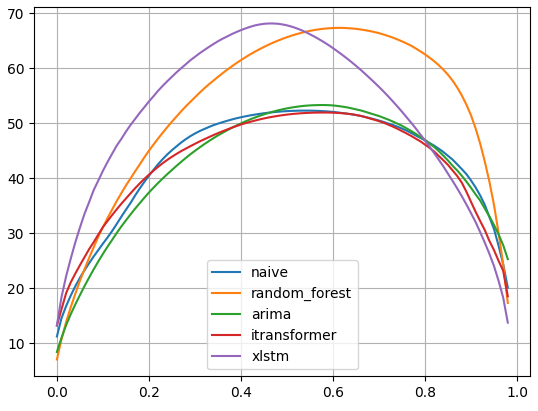
\includegraphics[width=\linewidth]{../images/results/quantile_pinball_scores.pdf}
  \caption{Quantile pinball scores for all models}
\end{subfigure}
\begin{subfigure}{0.45\textwidth}
  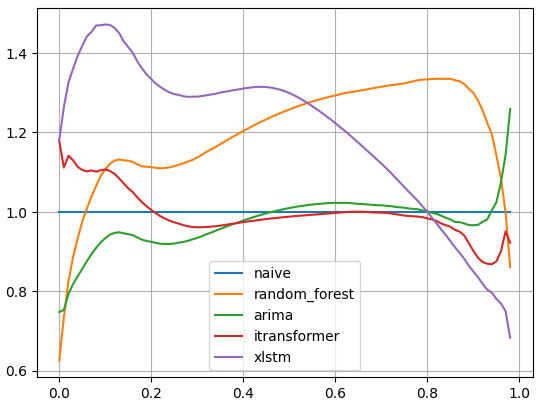
\includegraphics[width=\linewidth]{../images/results/quantile_pinball_scores_to_id1.pdf}
  \caption{Quantile pinball scores normalized based on naive}
\end{subfigure}
\caption{Quantile pinball scores for each model}
\label{Figure::pinball_scores}
\end{figure}


%Figure \ref{Figure::pinball_scores} shows the pinball scores for each quantile for each model.
%On the left the raw pinball scores are shown.
%The right graph shows the pinball score in relation to the pinball score of the naive model.
%These values are calculated by dividing the pinball score for each quantile $q$ for each model by the the pinball score for the quantile $q$ for the naive model.
%
%These charts show, that random forest performs the best on the lowest quantile and is among the best in the higher quantiles. 
%%Across most of the percentiles, from about $0.1$ to $0.8$ both random forest and xlstm have the worst pinball score.
%The xLSTM shines in the higher quantiles. 
%The pinball scores for xLSTM are the best in the higher percentiles. 
%This is in line with this model having the best RMSE, due to the nature of the otliers being very extreme.


%Figure \ref{Figure::Model_predictions} shows the predictions for the machine learning models on an example day and the actual imbalance price.

%\begin{figure}
%  \centering
%\begin{subfigure}{0.45\textwidth}
%  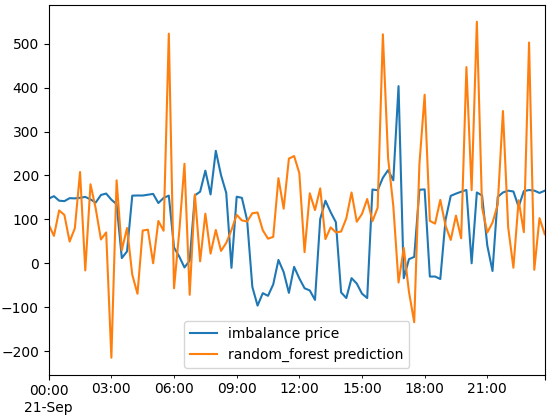
\includegraphics[width=\linewidth]{../images/results/random_forest_prediction.png}
%  \caption{Predictions of random forest}
%\end{subfigure}
%\begin{subfigure}{0.45\textwidth}
%  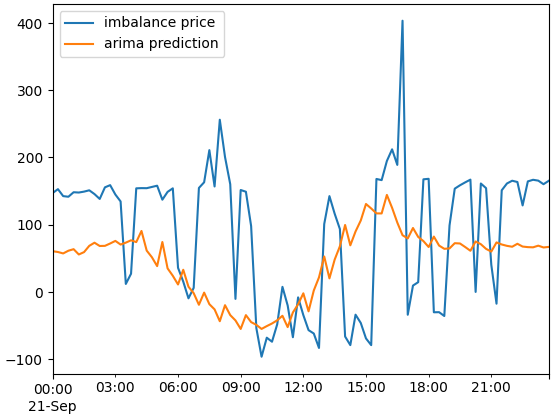
\includegraphics[width=\linewidth]{../images/results/arima_prediction.png}
%  \caption{Predictions of ARIMA}
%\end{subfigure}
%\begin{subfigure}{0.45\textwidth}
%  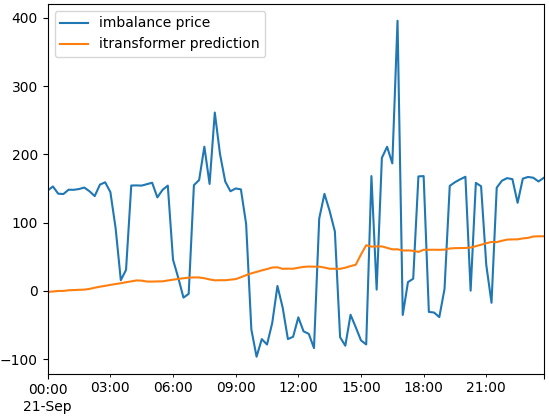
\includegraphics[width=\linewidth]{../images/results/itransformer_prediction.png}
%  \caption{Predictions of iTransformer}
%\end{subfigure}
%\begin{subfigure}{0.45\textwidth}
%  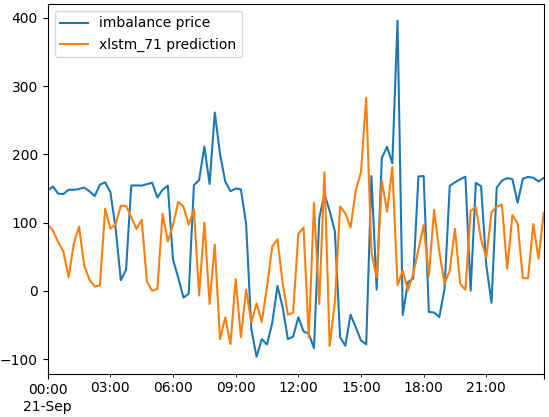
\includegraphics[width=\linewidth]{../images/results/xlstm_prediction.png}
%  \caption{Predictions of xLSTM}
%\end{subfigure}
%\caption{Predictions of the different models on example day}
%\label{Figure::Model_predictions}
%\end{figure}
%
%While random forest better predicticts the imbalance price with regards to mean average error, the xLSTM model seems to better capture outlieres, resulting in a lower mean %squared error.
%
%
\section{Different xLSTM block structures}

  \begin{table}[]
\centering
\begin{tabular}{l|l|l|l}
Configuration name 		&  RMSE 			 & MAE 			 & CRPS			\\\hline
xLSTM\_7\_1 4 seq		&$ 302.57\pm 6.68	$&$ \underline{84.33 \pm 1.17}	$&$ \underline{40.30	\pm0.24} $\\
xLSTM\_1\_0 96 seq		&$\underline{316.81\pm5.37} $&$ 85.68\pm 1.81	$& $40.34	\pm 0.32$\\
xLSTM\_1\_1 96 seq		&$ 318.48\pm12.03 	$&$87.73	\pm 3.16	$&$ 40.99	\pm 1.05$\\
xLSTM\_7\_1 96 seq	 	&$325.70 \pm5.56	$&$85.76\pm 2.09	$&$ 40.47	\pm 0.27$\\ 
\end{tabular}
\caption{Error metrics and CRPS for different xLSTM block configurations}
\label{Table::Performance_xLSTM}

\end{table}
\begin{table}
\centering
\begin{tabular}{l|l|l|l}
Configuration name 		& 50\%-cov 		& 90\%-cov 		& 98\%-cov \\\hline
xLSTM\_7\_1 4 seq	&$ 0.240 \pm 0.019	$&$ \underline{0.759 	\pm 0.012}	$&$ \underline{0.910 \pm 0.009}	 $\\
xLSTM\_1\_0 96 seq		&$\underline{ 0.277 \pm0.023}	$&$  0.743 \pm0.025	$&$ 0.886\pm0.028	$\\
xLSTM\_1\_1 96 seq		&$ 0.263 \pm0.046	$&$ 0.732 \pm0.044	$&$ 0.877\pm 0.032	$\\
xLSTM\_7\_1 96 seq	 	&$ 0.263 \pm0.021	$&$ 0.724 \pm0.014	$&$ 0.867 \pm0.010	$\\ 
\end{tabular}
\caption{Quantile metrics for different xLSTM block configurations}
\label{Table::Performance_xLSTM_quantile}
\end{table}
This experiment investigates how internal architectural choices in the xLSTM model — specifically the composition of mLSTM and sLSTM blocks — affect predictive performance. Tables \ref{Table::Performance_xLSTM} and \ref{Table::Performance_xLSTM_quantile} report the results for several variants, including the default 7\_1 configuration, as well as pure mLSTM (1\_0) and mixed (1\_1) structures. All models were trained with 96-step input sequences, except for the 7\_1 configuration with a short 4-step input, which serves as a reference for sequence length effects.

The results show that architectural variation has only a minor effect on forecasting performance. All 96-step configurations yield similar MAE (~85–88) and CRPS (~40.3–41.0), with no clear winner. The pure mLSTM model (1\_0) achieves the lowest RMSE (316.81) and best coverage (50\%-cov: 0.277), while the default mixed configuration (7\_1) performs slightly worse across all metrics.

Interestingly, the 4-sequence variant (7\_1) outperforms all 96-sequence models in both MAE (84.33) and CRPS (40.30), and reaches the highest coverage at the 90\% and 98\% levels. This suggests that shorter input sequences can yield sharper, more reactive forecasts, possibly by reducing over-smoothing and forcing the model to focus on the most recent dynamics. 

Overall, the results indicate that xLSTM performance is robust to architectural variation, and more sensitive to sequence length than to the internal mix of memory cell types.


\section{iTransformer variable sequence length}
This experiment investigates how the iTransformer model’s performance varies with different input sequence lengths. As shown in Tables \ref{Table::Performane_sequence_length} and \ref{Table::Performance_sequence_length2}, the model was evaluated using sequences of 4, 96, 192, and 384 time steps.

In terms of point forecast accuracy, longer input sequences do not lead to performance improvements. On the contrary, the shortest-sequence model (4 seq) achieves the lowest RMSE (200.19) and lowest MAE (139.87), despite having access to significantly less historical context. As sequence length increases, both MAE and RMSE deteriorate slightly, while CRPS increases notably, from 49.24 (4 seq) to 58.68 (384 seq).

This trend is even more pronounced in the quantile coverage metrics: the 4-sequence model attains the highest coverage across all levels (e.g. 90\%-cov = 0.841), while longer sequences exhibit steadily declining coverage, down to 0.282 at 90\% for the 384-step model. This suggests that longer sequence inputs lead the iTransformer to produce overconfident, underdispersed forecasts, which fail to reflect true uncertainty in imbalance price dynamics.

A possible explanation is that with longer inputs, the model tends to overfit to smoothed trends or ignore recent volatility, which reduces its responsiveness to short-term price spikes. 

Overall, these results imply that for the iTransformer architecture, shorter input sequences yield better-calibrated and more robust forecasts, particularly in capturing tail risk. This highlights a critical design consideration for sequence models: more historical context does not necessarily translate into better probabilistic performance — especially in volatile, regime-switching markets like imbalance pricing.

 \begin{table}[]
\centering
\begin{tabular}{l|l|l|l}
 Configuration name &  RMSE 		& MAE 			& CRPS \\\hline
iTransformer 4 seq    &$ 200.19 \pm 0.07	$&$ 139.87	\pm 0.06	$&$ \underline{49.24 \pm 0.04	}$ \\
 iTransformer 96 seq &$  \underline{186.15 \pm  0.12} $&$ \underline{135.78 \pm 0.06} $ &$  54.93\pm 0.02$\\
 iTransformer 192 seq &$ 188.02 \pm 0.01$ &$ 135.90 \pm 0.01$&$ 56.49 \pm0.13 $ \\
 iTransformer 384 seq &$ 188.16 \pm 0.58 $&$ 135.85 \pm 0.31 $&$ 58.68 \pm 0.11 $ \\
\end{tabular}
\caption{Error metrics and CRPS for different sequence lengths}
\label{Table::Performance_sequence_length}

\end{table}
\begin{table}
\centering
\begin{tabular}{l|l|l|l}
 Configuration name 	& 50\%-cov 		& 90\%-cov 		& 98\%-cov \\\hline
iTransformer  4 seq   	&$ \underline{0.356	\pm 0.001}$&$ \underline{0.841	\pm 0.000}	$&$\underline{0.959 \pm 0.000}	$ \\
 iTransformer 96 seq 	&$ 0.088 \pm 0.004$&$ 0.540 \pm 0.012$ 	&$ 0.755 \pm 0.003$ \\
 iTransformer 192 seq 	&$ 0.072 \pm 0.002$&$ 0.415\pm 0.016$ 	&$ 0.660 \pm 0.008$ \\
 iTransformer 384 seq 	&$ 0.049 \pm 0.002 $&$ 0.282 \pm 0.011$	&$ 0.475 \pm 0.030$\\
\end{tabular}
\caption{Quantile metrics for for different sequence lengths}
\label{Table::Performance_sequence_length2}
\end{table}



\section{iTransformer multiple target variables}

This experiment evaluates whether the iTransformer benefits from multi-target learning, i.e., jointly forecasting imbalance price along with additional target variables such as intraday indices, ENTSO-E physical data, and Netzregelverbund indicators. Table \ref{Table::Performance_targets} compares the predictive performance of models trained on different target combinations, including a combined configuration encompassing all auxiliary series.

Across all setups, no substantial performance improvements are observed. All variants achieve nearly identical RMSE (~185.5–186.0), MAE (~135.4–135.8), and CRPS (~54.8–54.9). Similarly, Table \ref{Table::Performance_targets2} shows minimal variation in quantile coverage metrics, with the combined model performing only marginally better at the 50\%-level (0.098) but showing no consistent gains at higher coverage levels.

These results suggest that the selected auxiliary targets — while related to the system state — do not provide additional predictive structure that improves the reBAP forecast. A likely reason is that these variables either correlate only weakly with the imbalance price or introduce noise that dilutes the learning signal for the main target.

Overall, this experiment indicates that multi-target learning does not enhance performance in this setting, and that focused single-target modeling may be preferable for probabilistic imbalance price forecasting — unless better-aligned or more informative auxiliary variables can be identified.

 \begin{table}[]
\centering
\begin{tabular}{l|l|l|l}
 Configuration name			&  RMSE 			& MAE 			& CRPS 			 \\\hline
 iTransformer intraday indices 		&$ 185.95\pm 0.46	$&$ 135.67 \pm 0.30	$&$ 54.84\pm0.17	$\\
 iTransformer entsoe data		&$  185.95 \pm 0.38 $&$ 135.65 \pm 0.19		$&$ 54.93 \pm 0.011		 $\\
 iTransformer netzregelverbund 	& $186.05 \pm 0.35	$&$ 135.80\pm0.27	$&$ 54.90\pm 0.02	$\\
 iTransformer combined 		&$ \underline{185.52 \pm 0.93}	$&$ \underline{135.36\pm 0.61}	$&$ \underline{54.81\pm 0.18	2} $\\
\end{tabular}
\caption{Error metrics and CRPS for multiple target variables}
\label{Table::Performance_targets}
\end{table}
\begin{table}
\centering
\begin{tabular}{l|l|l|l}
 Configuration name			& 50\%-cov 		& 90\%-cov 		& 98\%-cov \\\hline
 iTransformer intraday indices 		&$0.090\pm 0.009	$& $0.546\pm 0.011	$ & $0.755 \pm 0.002$\\
 iTransformer entsoe data		&$0.090 \pm  0.002	$&$ 0.533 \pm 0.004	$&$0.755 \pm 0.006 $\\
 iTransformer netzregelverbund 	&$0.085\pm 0.004	$&$\underline{0.551 \pm 0.010}	$&$ 0.750 \pm 0.003$\\
 iTransformer combined 		&$ \underline{0.098\pm 0.015}	$&$ 0.542 \pm 0.018 	$&$ \underline{0.755 \pm 0.003}$\\
\end{tabular}
\caption{Quantile metrics for for  multiple target variables}
\label{Table::Performance_targets2}
\end{table}


%\begin{figure}
% % \centering
%\begin{subfigure}{0.45\textwidth}
%  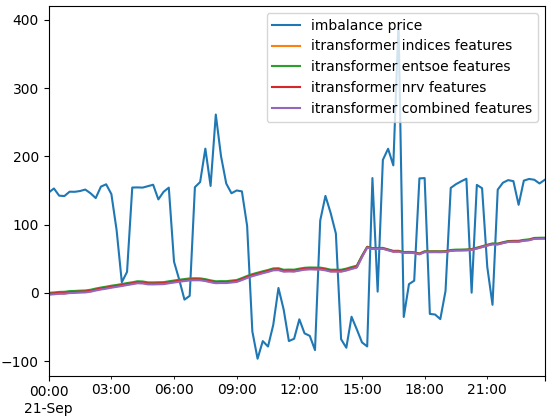
\includegraphics[width=\linewidth]{../images/results/itransformer_target_variables_aep.png}
%  \caption{Predictions of models with imbalance price}
%\end{subfigure}
%\begin{subfigure}{0.45\textwidth}
%  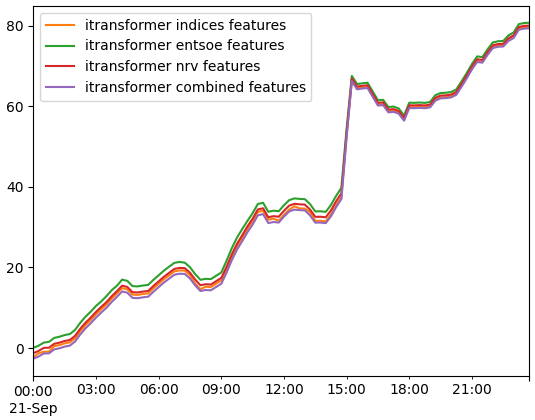
\includegraphics[width=\linewidth]{../images/results/itransformer_target_variables_alone.png}
%  \caption{Predictions of models without imbalance price}
%\end{subfigure}
%\caption{Predictions of iTransformers trained on multiple target variables}
%\label{Figure::Targets_prediction}
%\end{figure}


\section{iTransformer different prediction horizons}
This experiment explores whether training the iTransformer to forecast longer horizons improves its ability to predict the one-hour-ahead imbalance price. The model was trained with forecast horizons of 4, 12, 24, 48, and 96 steps, and evaluated solely on the one-hour-ahead target.

As shown in Tables \ref{Table::Performance_targets_horizon} and \ref{Table::Performance_targets_horizon2}, all configurations perform nearly identically. Differences in RMSE, MAE, and CRPS across horizons are minimal (less than 0.3 points in each metric), and quantile coverage metrics vary only in the third decimal place. The longest-horizon model (96 steps) does not outperform shorter-horizon models — in fact, it shows slightly worse MAE (135.99) and CRPS (54.94), though the differences are insignificant.

These results suggest that longer forecast horizons do not yield any benefit for short-term imbalance price prediction in this setup. A likely explanation is that the model is trained to optimize the entire sequence output, which can dilute the learning focus on the one-hour-ahead value. Additionally, longer sequences may introduce training complexity without additional relevant signal.

This experiment implies that training the model specifically for the target horizon is sufficient, and that increasing the output range does not lead to generalization gains

 \begin{table}[]
\centering
\begin{tabular}{l|l|l|l}
 Configuration name			&  RMSE 			& MAE 			& CRPS 	\\\hline
 iTransformer 4 horizon		& $\underline{186.16 \pm 0.02}	$&$ 135.79 \pm 0.03	$&$54.92 \pm 0.01$\\
 iTransformer 12 horizon		&$ 186.24\pm 0.11	$&$135.89 \pm 0.14	$&$54.89 \pm 0.02$ \\
 iTransformer 24 horizon		&$ 186.17	\pm 0.01	$&$ \underline{135.76 \pm 0.03}	$&$54.89	\pm 0.01$\\
 iTransformer 48 horizon		&$ 186.22  \pm 0.03	$&$\underline{ 135.76 \pm 0.04	}$&$\underline{54.88	\pm 0.00}$ \\
 iTransformer 96 horizon		&$ 186.47	\pm 0.01	$&$ 135.99 \pm 0.02	$&$54.94	\pm 0.00$\\
\end{tabular}
\caption{iTransformer performance for multiple target variables}
\label{Table::Performance_targets_horizon}
\end{table}
\begin{table}
\centering
\begin{tabular}{l|l|l|l}
 Configuration name			&   50\%-cov 		& 90\%-cov 		& 98\%-cov \\\hline
 iTransformer 4 horizon		&$\underline{0.086 \pm 0.001}	$&$ 0.541\pm 0.003 	$&$\underline{0.756 \pm 0.001}$\\
 iTransformer 12 horizon		&$0.084\pm 0.002	$&$ \underline{0.549\pm 0.009}	$ &$ 0.753 \pm 0.003$ \\
 iTransformer 24 horizon		&$0.084\pm 0.001	$&$0.543\pm 0.002	 $&$0.755 \pm 0.001$\\
 iTransformer 48 horizon		&$0.085\pm 0.001	$&$ 0.543\pm 0.002	 $&$\underline{ 0.756\pm 0.001}$ \\
 iTransformer 96 horizon		&$0.083\pm 0.000	$&$ 0.544\pm 0.001	 $&$ \underline{0.756 \pm 0.000}$\\
\end{tabular}
\caption{iTransformer performance for multiple target variables}
\label{Table::Performance_targets_horizon2}
\end{table}

%\begin{figure}
%  \centering
%\begin{subfigure}{0.45\textwidth}
%  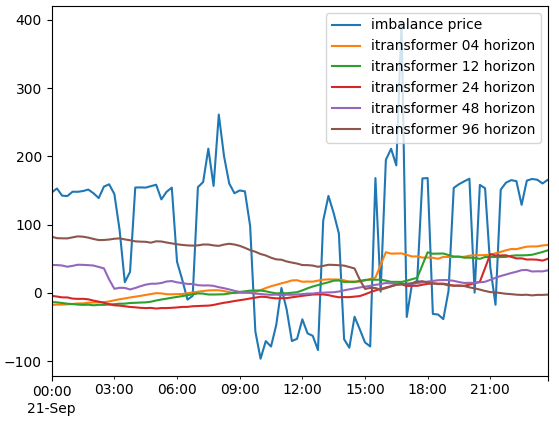
\includegraphics[width=\linewidth]{../images/results/itransformer_horizon_lengths.png}
%  \caption{Predictions of models with imbalance price}
%\end{subfigure}
%\begin{subfigure}{0.45\textwidth}
%  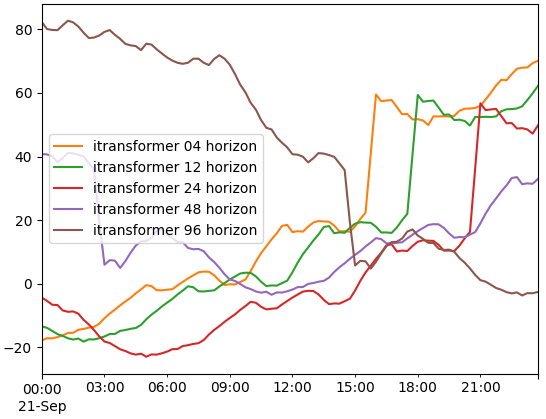
\includegraphics[width=\linewidth]{../images/results/itransformer_horizon_lengths_alone.png}
%  \caption{Predictions of models without imbalance price}
%\end{subfigure}
%\caption{Predictions of iTransformers trained on different forecasting horizons}
%\label{fig:fig}
%\end{figure}


\section{Feature Importance: Insights from Random Forest}
\label{Section::Analysis or Evaluation of Something}    


Table  \ref{Table::Feature_importance} lists the 15 most important input features used by the Random Forest model, aggregated across time-shifted variants. The top-ranked features are dominated by market price signals, most notably the hourly spot price and IDA1, which stand out with clearly higher importance values than the rest. This underscores the strong influence of recent and forward market indicators in reBAP prediction.

Subsequent features — including lagged intraday indices (IDFULL, ID3, ID1), the AEP schätzer, and fossil generation metrics (hard coal, lignite) — show a more gradual decline in importance, suggesting that a moderately wide set of features contributes meaningfully to the model’s performance. In particular, forecasted residual load stands out over shifted or error-based versions, indicating that forward-looking demand-supply imbalances are more informative than retrospective deviations.

Weather-related variables such as temperature at 1m depth, wet temperature, and wind offshore forecast error also appear in the top 15. The presence of forecasting errors over raw values for wind points to the importance of uncertainty signals from volatile renewables.

Overall, the results suggest that the Random Forest relies on a core set of market-driven features, supported by operational and meteorological indicators. Rather than focusing on a narrow subset, the model balances high-impact features with a broader context, reflecting the multifactorial nature of imbalance price formation.



%Table \ref{Table::Feature_importance} contains information about the most important features for the random forest prediction.
%The top 6 most important features consist of information about prices. Interesting is, that the intraday index shifted by one day still has a very high feature importance.
%The next two most important features \textit{lignite actual generation shifted by 30 minuts} and \textit{fossil hard coal actual generation shifted 30 minutes} contain %information about generated energy provided by fossil energy sources.
%The third features containing information about fossil energy sources ranks 14\textsuperscript{th} most important. 
%The importance of features doesn't change much after the  10\textsuperscript{th} most important feature.
%Out of the wheather data the temperature was the most important, followed by the difference in forecast for the solar radiation within one hour.
%Notable information from this importance is that the forecasted residual load is more important to the model than the shifted actual residual load or the shifted forecasting %error.
%For solar and wind offshore generation the opposite is true. 
%The shifted forecasting error is more important than both the forecast and the shifted actual measurement.

\begin{table}[]
\centering
\begin{tabular}{l|l|l}
 Feature rank & Parameter & Importance \\\hline
 1-5 & Hourly spot price& 0.0970\\
 6-9, 14& IDA1&0.0582 \\
 12, 15, 16, 17, 40&intraday IDFULL shifted 1 day & 0.0306 \\
 10, 19, 21, 26, 32  &aep schaetzer shifted 30 minutes&0.0303\\
 11, 20, 24, 25, 29 &intraday ID3 shifted 1 day &0.0283\\
 13, 18, 22, 23, 69 & intraday ID1 shifted 1 day &0.0271\\
 27, 28, 31, 46, 71 & entsoe fossil hard coal actual generation & 0.0203\\
 30, 34, 35, 36, 39 & entsoe lignite actual generation & 0.0196 \\
 33, 37, 41, 48, 66 & forecasted residual load & 0.0177 \\
 38, 51, 52, 85, 98 & entsoe wind onshore actual & 0.0154 \\
42, 57, 65, 75, 80 & entsoe fossil gas actual generation & 0.0151 \\
44, 61, 63, 70, 141 & dwd measurements temperatur in 1m depth & 0.0145 \\
55, 62, 67, 87, 93 & dwd measurements wet temperature & 0.0143 \\
58, 76, 81, 101, 118 & wind offshore forecasting error & 0.0135 \\
 
\end{tabular}
\caption{15 most important features of random forest sorted from most important to least important. For each feature all shifted values are aggregated to get the importance.}
\label{Table::Feature_importance}
\end{table}


\end{document}
 		 \clearpage
   % \documentclass[class=scrbook, crop=false]{standalone}
\usepackage[subpreambles=true]{standalone}
\ifstandalone
    % WARNING: Proceed with caution!

% -----------------------------------------------------------------------------------
% For package standalone
% -----------------------------------------------------------------------------------
\usepackage{import}

% -----------------------------------------------------------------------------------
% Language and typeset
% -----------------------------------------------------------------------------------
\usepackage[ngerman, english]{babel}

\usepackage{subcaption}
% Umlauts and other special characters (UTF-8)
% \usepackage[utf8]{inputenc}
\usepackage{fontspec}
\setsansfont{Arial}
% \usepackage[T1]{fontenc}  % Enable accented characters and umlauts
% LuaLatex doesn't need fontenc and uses UTF-8
% \usepackage{lmodern}  % Font face


% --------------------------------------------------------------------------------
% Page formatting
% --------------------------------------------------------------------------------
% Change the header/footer for chapter beginnings and normal pages
\usepackage[automark,headsepline]{scrlayer-scrpage}

% The package provides an easy and flexible user interface to customize the page
% layout, implementing auto-centering and auto-balancing mechanisms
% WARNING: WHEN CHANGING BCOR (Binding correction), the cover needs reworking!...
\newcommand{\theBCOR}{15mm}  % Define binding correction
\usepackage[
    bindingoffset=\theBCOR,
    % showframe, % Show boxes which indicate margins and paddings
    bottom = 3.5cm, % Margins
      left = 2.5cm,
     right = 2.5cm
] {geometry}

% The package 'float' provides a container for document objects which can not be
% broken over pages, such as tables and figures
% Needed for table and figure indexes  
\usepackage{float}

% support for landscape layout
\usepackage{lscape}

% support of \tablenotes command to add notes under table
\usepackage{threeparttable}

% To allow drawing more professional tables
\usepackage{booktabs}

% --------------------------------------------------------------------------------
% Contents
% --------------------------------------------------------------------------------
% Vector graphics (for Cover page)
\usepackage{tikz} 

% Allows additional parameters when including images
\usepackage{graphicx}

% Roman font family for all headings
\addtokomafont{disposition}{\rmfamily}

% Set the line spacing to 1.5
\usepackage[onehalfspacing]{setspace}

% Improves overall text spacing
% http://www.khirevich.com/latex/microtype/
\usepackage[stretch=10]{microtype}

% Math symbols like mu outside the math environment
\usepackage{textcomp}

% A comprehensive (SI) units package∗
% For defining SI units
\usepackage[
    range-units=single,         % Formatting ranges with single unit indication: 1 - 2 m
    range-phrase=-,             % Phrase for range: 1 - 2 m vs 1 to 2 m
    separate-uncertainty=true,  % sets +- between value and uncertainty 
    multi-part-units=repeat     % In expressions with multiple values (multi part numbers) 
                                % the unit is printed each time: 1 mm x 1 mm
] {siunitx}
% https://tex.stackexchange.com/questions/124488/multi-part-numbers-and-units-in-siunitx

% Allows Sourcecodes with highlighting 
\usepackage{listings}

% This package provides user control over the layout of the three basic list
% environments: enumerate, itemize and description
\usepackage{enumitem}
\setlist{nosep} % Remove the vertical space between \item elements in all lists

% ToDo Notes
% \setlength{\marginparwidth}{2cm}
\usepackage{todonotes}
\setuptodonotes{inline, inlinepar}
\reversemarginpar  % Put ToDo notes on the binding's side
% \usepackage{soul} % Colorful ToDo notes

% Check out colors here http://latexcolor.com/
\usepackage{xcolor}

\usepackage{amsmath}    % alignment of equations

% --------------------------------------------------------------------------------
% Other elements
% --------------------------------------------------------------------------------
% Blindtext: Organic looking text dummy
\usepackage{blindtext}

% Hyperlinks within the document (PDF)
% "hidelinks" hides visual highlighting of links
\usepackage[hidelinks]{hyperref}

% Package for Glossary and Index (Acronyms are listed in a separate list) 
\usepackage[acronym, nogroupskip]{glossaries}[=v4.49] % groupskip: alphabetic grouping of entries

\usepackage{xltabular}   % <------- FOR glossaries

% Integration and management of bibliographies
\usepackage{csquotes}   % backend=biber in biblatex needs this package
\usepackage[
    style=ieee,   % style of the bibliography, entries are sorted in alphabetic order. "ieee" is another common style.
    backend=biber,      % based on package 'biber' 
    bibencoding=ascii   % ASCII Text encoding; may use "utf8" instead
] {biblatex}

% --------------------------------------------------------------------------------
%                               PATHS & FILES
% --------------------------------------------------------------------------------
% Fix paths for standalone compiling
\ifstandalone
    \def \home {..}
\else
    \def \home {.}
\fi

% Package: scrlayer-scrpage
% \def \stylePath {\home/settings+/style/page}
\input{\home/settings+/style/page}  % Load page style

% Package: graphicx
\graphicspath{{\home/images/}}  % Set path to images

% Package: listings
\input{\home/settings+/style/code.tex}  % Set path to style file
\lstset{inputpath={\home/code/}} % Default path to code listings

% Package: glossaries
\input{\home/settings+/style/symbols}  % Set path to symbols list style file
\input{\home/settings+/style/acronyms}  % Set path to acronym list style file
% -------------------------------------------------------------------------------
%               Listing of all Glossary and Acronym Entries 
%                           use as shown below
% -------------------------------------------------------------------------------

% ==== EXEMPLARY ENTRY FOR SYMBOLS LIST =========================================

% ==== EXEMPLARY ENTRY FOR ACRONYMS LIST ========================================
% \newacronym{#label}{#acronym}{#long_form}

% define new command for custom arconym entry with only two arguments
% fabricates an easier way to use \newacronym 
\newcommand{\acroX}[2]{\newacronym{#1}{#1}{#2}}
% \acroX{label and arconym}{long name}
% \acroX{CD}               {Compact Disk}

\newcommand{\acroY}[3]{\newacronym{#1}{#2}{#3}}
% \arcoY{label}{acronym}{long name}
% \acroY{CD}   {cd}     {Compact Disk}
 
\newacronym{AEP}{AEP}{Imbalance price}
\newacronym{aFRR}{aFRR}{Automatic Frequency Restoration Reserve}


\newacronym{reBAP}{reBAP}{Uniform imbalance price}
\newacronym{TSO}{TSO}{Transmission System Operator}
\newacronym{FCR}{FCR}{Frequency Containment Reserve}
\newacronym{mFRR}{mFRR}{Manual Frequency Restoration Reserve}
\newacronym{BRP}{BRP}{Balancing Responsible Party}
\newacronym{SB}{SB}{System Balance}
\newacronym{VRE}{VRE}{variable renewable energy}
\newacronym{ID1}{ID1}{intraday index ID1}
\newacronym{MAE}{MAE}{mean average error}
\newacronym{RMSE}{RMSE}{root mean squared error}
\newacronym{MSE}{MSE}{mean squared error}
\newacronym{CRPS}{CRPS}{continuous ranked probabililty score}
\newacronym{GCC}{GCC}{Grid Control Cooperation}
\newacronym{IC}{IC}{Continuous intraday}
\newacronym{VWAP}{VWAP}{volume-weighted average price}
\newacronym{VID}{VID}{traded volume within the intraday market}
\newacronym{ID AEP}{ID AEP}{Intraday Average Energy Price}
\newacronym{FRR}{FRR}{Frequency Restoration Reserve}
\newacronym{TFT}{TFT}{Temporal Fusion Transformer}
\newacronym{DLM}{DLM}{Dynamic Linear Model}
\newacronym{GB}{GB}{Gradient Boosting}
\newacronym{RF}{RF}{Random Forest}
\newacronym{ARIMAX}{ARIMAX}{Autoregressive Integrated Moving Average with eXogenous variables}
\newacronym{xLSTM}{xLSTM}{Extended Long Short-Term Memory}
\newacronym{DWD}{DWD}{Deutscher Wetterdienst}
\newacronym{ENTSO-E}{ENTSO-E}{European Network of Transmission System Operators for Electricity}
\newacronym{IDA1}{IDA1}{Intraday auction 1}
\newacronym{MOSMIX}{MOSMIX}{Model Output Statistics-MIX}
\newacronym{mLSTM}{mLSTM}{memory-optimized LSTM}
\newacronym{sLSTM}{sLSTM}{speed-optimized LSTM}

% ==== EXEMPLARY ENTRY FOR MAIN GLOSSARY ========================================

    % \newglossaryentry{policy}{name={Policy},description={Im geschäftlichen Bereich bezeichnet Policy eine interne Leit- bzw. Richtlinie, die formal durch das Unternehmen dokumentiert und über ihr Management verantwortet wird}}
    % \newglossaryentry{pcie}{name={PCI Express},description={PCI Express („Peripheral Component Interconnect Express“, abgekürzt PCIe oder PCI-E) ist ein Standard zur Verbindung von Peripheriegeräten mit dem Chipsatz eines Hauptprozessors. PCIe ist der Nachfolger von PCI, PCI-X und AGP und bietet im Vergleich zu seinen Vorgängern eine höhere Datenübertragungsrate pro Pin.}}
    % \newglossaryentry{realnumber}
  % Load glossary, symbol and acronyms list

% Package: biblatex
\addbibresource{\home/references/references.bib}  % Set path to bib resources

% Custom variables
\input{\home/settings+/variables}
% --------------------------------------------------------------------------------
%                                   OPTIONAL
% --------------------------------------------------------------------------------


% Simple arithmetic for LaTeX commands
% \usepackage{calc}

% Document Elements
% -------------------

% Index
% \usepackage{imakeidx}

% compact Lists
%\usepackage{paralist}

% visual improvements for citations
% \usepackage{epigraph}

% Create pseudo code
% https://www.overleaf.com/learn/latex/Algorithms
% \usepackage{algorithm}
% \usepackage{algorithmic}
%\usepackage[noend]{algpseudocode}

% Formatting
% -------------------
% Tweaks for scrbook, redefines commands of other packages
% \usepackage{scrhack}

% Intelligent space separator (nice for superscript?)
% \usepackage{xspace}

% Allows breaks within tables
%\usepackage{tabularx}

% Allows for page breaks in tables
% \usepackage{longtable}

% allows modifying of captions
% \usepackage{caption}

% Multiline comments
%\usepackage{verbatim}

% % Custom colors
% \definecolor{dartmouthgreen}{rgb}{0.05, 0.5, 0.06}

% IF you want to define unicode characters
% \DeclareUnicodeCharacter{0229}{\c{e}}
% \DeclareUnicodeCharacter{0306}{\u{Z}}


% Document elements
% ------------------------------------

% Table package
% \usepackage{booktabs}

% Pie diagram
% \usepackage{datapie}

% Side by Side images
% \usepackage{subcaption}

% For landscape tables
%\usepackage{pdflscape}
%\usepackage{afterpage}

% Graphics can be flow around by text
%\usepackage{wrapfig}

\fi

% ----------------------------------------------------------------------------
%                               Summary
% ----------------------------------------------------------------------------
\begin{document}

\chapter{Summary}
\label{Chapter::Summary}
    In this chapter, there is a short summary? results of the thesis are presented and evaluated as well as, the approach of this thesis.

In the experiments random forest performed remarkably well. 
When looking at MAE it outperformed all the other models. 
This might be due to the additional information passed to random forest. 
Only random forest and ARIMA received information about past days and past weeks for the same timestamp. 
With Load and Generation behaving periodically with a period of one day and one week, this information might have a large impact.

The ARIMA model has access to the same information but the model does not seem to be able to capture the complexity of the time series.
Another reason why random forest outperformed the other models is because the hyperparameters were tuned a little. 
For this method the best model was determined by using random search, testing 20 different configurations in the process.
The hyperparameter tuning used tried to reduce mean squared error.

This makes it more impressing that xLSTM has a lower RMSE than random forest, even without hyper parameter tuning.

Most of the models were not able to beat the naive intraday index ID1 when looking at MAE. 
This might be due to the fact that information about current prices are lacking. 
The ID1 is composed of market decisions done by BRPs, which have access to market prices.
Additionally no information about balancing reserves was included in the training process for the machine learning models.

The performance of the more complex time series predictors can also be explained by the lack of hyperparameter tuning. 


% Show your results and analyze them
% Explain why the results are the way they are and not different
% Go into possible measurement errors and why they occurred
% Look for anomalies and explain why they occur
\section{Analysis or Evaluation of Something}
\label{Section::Short Analysis or Evaluation of Something}    
    Text

\end{document}
                                              \clearpage
    \documentclass[class=scrbook, crop=false]{standalone}
\usepackage[subpreambles=true]{standalone}
\ifstandalone
    % WARNING: Proceed with caution!

% -----------------------------------------------------------------------------------
% For package standalone
% -----------------------------------------------------------------------------------
\usepackage{import}

% -----------------------------------------------------------------------------------
% Language and typeset
% -----------------------------------------------------------------------------------
\usepackage[ngerman, english]{babel}

\usepackage{subcaption}
% Umlauts and other special characters (UTF-8)
% \usepackage[utf8]{inputenc}
\usepackage{fontspec}
\setsansfont{Arial}
% \usepackage[T1]{fontenc}  % Enable accented characters and umlauts
% LuaLatex doesn't need fontenc and uses UTF-8
% \usepackage{lmodern}  % Font face


% --------------------------------------------------------------------------------
% Page formatting
% --------------------------------------------------------------------------------
% Change the header/footer for chapter beginnings and normal pages
\usepackage[automark,headsepline]{scrlayer-scrpage}

% The package provides an easy and flexible user interface to customize the page
% layout, implementing auto-centering and auto-balancing mechanisms
% WARNING: WHEN CHANGING BCOR (Binding correction), the cover needs reworking!...
\newcommand{\theBCOR}{15mm}  % Define binding correction
\usepackage[
    bindingoffset=\theBCOR,
    % showframe, % Show boxes which indicate margins and paddings
    bottom = 3.5cm, % Margins
      left = 2.5cm,
     right = 2.5cm
] {geometry}

% The package 'float' provides a container for document objects which can not be
% broken over pages, such as tables and figures
% Needed for table and figure indexes  
\usepackage{float}

% support for landscape layout
\usepackage{lscape}

% support of \tablenotes command to add notes under table
\usepackage{threeparttable}

% To allow drawing more professional tables
\usepackage{booktabs}

% --------------------------------------------------------------------------------
% Contents
% --------------------------------------------------------------------------------
% Vector graphics (for Cover page)
\usepackage{tikz} 

% Allows additional parameters when including images
\usepackage{graphicx}

% Roman font family for all headings
\addtokomafont{disposition}{\rmfamily}

% Set the line spacing to 1.5
\usepackage[onehalfspacing]{setspace}

% Improves overall text spacing
% http://www.khirevich.com/latex/microtype/
\usepackage[stretch=10]{microtype}

% Math symbols like mu outside the math environment
\usepackage{textcomp}

% A comprehensive (SI) units package∗
% For defining SI units
\usepackage[
    range-units=single,         % Formatting ranges with single unit indication: 1 - 2 m
    range-phrase=-,             % Phrase for range: 1 - 2 m vs 1 to 2 m
    separate-uncertainty=true,  % sets +- between value and uncertainty 
    multi-part-units=repeat     % In expressions with multiple values (multi part numbers) 
                                % the unit is printed each time: 1 mm x 1 mm
] {siunitx}
% https://tex.stackexchange.com/questions/124488/multi-part-numbers-and-units-in-siunitx

% Allows Sourcecodes with highlighting 
\usepackage{listings}

% This package provides user control over the layout of the three basic list
% environments: enumerate, itemize and description
\usepackage{enumitem}
\setlist{nosep} % Remove the vertical space between \item elements in all lists

% ToDo Notes
% \setlength{\marginparwidth}{2cm}
\usepackage{todonotes}
\setuptodonotes{inline, inlinepar}
\reversemarginpar  % Put ToDo notes on the binding's side
% \usepackage{soul} % Colorful ToDo notes

% Check out colors here http://latexcolor.com/
\usepackage{xcolor}

\usepackage{amsmath}    % alignment of equations

% --------------------------------------------------------------------------------
% Other elements
% --------------------------------------------------------------------------------
% Blindtext: Organic looking text dummy
\usepackage{blindtext}

% Hyperlinks within the document (PDF)
% "hidelinks" hides visual highlighting of links
\usepackage[hidelinks]{hyperref}

% Package for Glossary and Index (Acronyms are listed in a separate list) 
\usepackage[acronym, nogroupskip]{glossaries}[=v4.49] % groupskip: alphabetic grouping of entries

\usepackage{xltabular}   % <------- FOR glossaries

% Integration and management of bibliographies
\usepackage{csquotes}   % backend=biber in biblatex needs this package
\usepackage[
    style=ieee,   % style of the bibliography, entries are sorted in alphabetic order. "ieee" is another common style.
    backend=biber,      % based on package 'biber' 
    bibencoding=ascii   % ASCII Text encoding; may use "utf8" instead
] {biblatex}

% --------------------------------------------------------------------------------
%                               PATHS & FILES
% --------------------------------------------------------------------------------
% Fix paths for standalone compiling
\ifstandalone
    \def \home {..}
\else
    \def \home {.}
\fi

% Package: scrlayer-scrpage
% \def \stylePath {\home/settings+/style/page}
\input{\home/settings+/style/page}  % Load page style

% Package: graphicx
\graphicspath{{\home/images/}}  % Set path to images

% Package: listings
\input{\home/settings+/style/code.tex}  % Set path to style file
\lstset{inputpath={\home/code/}} % Default path to code listings

% Package: glossaries
\input{\home/settings+/style/symbols}  % Set path to symbols list style file
\input{\home/settings+/style/acronyms}  % Set path to acronym list style file
% -------------------------------------------------------------------------------
%               Listing of all Glossary and Acronym Entries 
%                           use as shown below
% -------------------------------------------------------------------------------

% ==== EXEMPLARY ENTRY FOR SYMBOLS LIST =========================================

% ==== EXEMPLARY ENTRY FOR ACRONYMS LIST ========================================
% \newacronym{#label}{#acronym}{#long_form}

% define new command for custom arconym entry with only two arguments
% fabricates an easier way to use \newacronym 
\newcommand{\acroX}[2]{\newacronym{#1}{#1}{#2}}
% \acroX{label and arconym}{long name}
% \acroX{CD}               {Compact Disk}

\newcommand{\acroY}[3]{\newacronym{#1}{#2}{#3}}
% \arcoY{label}{acronym}{long name}
% \acroY{CD}   {cd}     {Compact Disk}
 
\newacronym{AEP}{AEP}{Imbalance price}
\newacronym{aFRR}{aFRR}{Automatic Frequency Restoration Reserve}


\newacronym{reBAP}{reBAP}{Uniform imbalance price}
\newacronym{TSO}{TSO}{Transmission System Operator}
\newacronym{FCR}{FCR}{Frequency Containment Reserve}
\newacronym{mFRR}{mFRR}{Manual Frequency Restoration Reserve}
\newacronym{BRP}{BRP}{Balancing Responsible Party}
\newacronym{SB}{SB}{System Balance}
\newacronym{VRE}{VRE}{variable renewable energy}
\newacronym{ID1}{ID1}{intraday index ID1}
\newacronym{MAE}{MAE}{mean average error}
\newacronym{RMSE}{RMSE}{root mean squared error}
\newacronym{MSE}{MSE}{mean squared error}
\newacronym{CRPS}{CRPS}{continuous ranked probabililty score}
\newacronym{GCC}{GCC}{Grid Control Cooperation}
\newacronym{IC}{IC}{Continuous intraday}
\newacronym{VWAP}{VWAP}{volume-weighted average price}
\newacronym{VID}{VID}{traded volume within the intraday market}
\newacronym{ID AEP}{ID AEP}{Intraday Average Energy Price}
\newacronym{FRR}{FRR}{Frequency Restoration Reserve}
\newacronym{TFT}{TFT}{Temporal Fusion Transformer}
\newacronym{DLM}{DLM}{Dynamic Linear Model}
\newacronym{GB}{GB}{Gradient Boosting}
\newacronym{RF}{RF}{Random Forest}
\newacronym{ARIMAX}{ARIMAX}{Autoregressive Integrated Moving Average with eXogenous variables}
\newacronym{xLSTM}{xLSTM}{Extended Long Short-Term Memory}
\newacronym{DWD}{DWD}{Deutscher Wetterdienst}
\newacronym{ENTSO-E}{ENTSO-E}{European Network of Transmission System Operators for Electricity}
\newacronym{IDA1}{IDA1}{Intraday auction 1}
\newacronym{MOSMIX}{MOSMIX}{Model Output Statistics-MIX}
\newacronym{mLSTM}{mLSTM}{memory-optimized LSTM}
\newacronym{sLSTM}{sLSTM}{speed-optimized LSTM}

% ==== EXEMPLARY ENTRY FOR MAIN GLOSSARY ========================================

    % \newglossaryentry{policy}{name={Policy},description={Im geschäftlichen Bereich bezeichnet Policy eine interne Leit- bzw. Richtlinie, die formal durch das Unternehmen dokumentiert und über ihr Management verantwortet wird}}
    % \newglossaryentry{pcie}{name={PCI Express},description={PCI Express („Peripheral Component Interconnect Express“, abgekürzt PCIe oder PCI-E) ist ein Standard zur Verbindung von Peripheriegeräten mit dem Chipsatz eines Hauptprozessors. PCIe ist der Nachfolger von PCI, PCI-X und AGP und bietet im Vergleich zu seinen Vorgängern eine höhere Datenübertragungsrate pro Pin.}}
    % \newglossaryentry{realnumber}
  % Load glossary, symbol and acronyms list

% Package: biblatex
\addbibresource{\home/references/references.bib}  % Set path to bib resources

% Custom variables
\input{\home/settings+/variables}
% --------------------------------------------------------------------------------
%                                   OPTIONAL
% --------------------------------------------------------------------------------


% Simple arithmetic for LaTeX commands
% \usepackage{calc}

% Document Elements
% -------------------

% Index
% \usepackage{imakeidx}

% compact Lists
%\usepackage{paralist}

% visual improvements for citations
% \usepackage{epigraph}

% Create pseudo code
% https://www.overleaf.com/learn/latex/Algorithms
% \usepackage{algorithm}
% \usepackage{algorithmic}
%\usepackage[noend]{algpseudocode}

% Formatting
% -------------------
% Tweaks for scrbook, redefines commands of other packages
% \usepackage{scrhack}

% Intelligent space separator (nice for superscript?)
% \usepackage{xspace}

% Allows breaks within tables
%\usepackage{tabularx}

% Allows for page breaks in tables
% \usepackage{longtable}

% allows modifying of captions
% \usepackage{caption}

% Multiline comments
%\usepackage{verbatim}

% % Custom colors
% \definecolor{dartmouthgreen}{rgb}{0.05, 0.5, 0.06}

% IF you want to define unicode characters
% \DeclareUnicodeCharacter{0229}{\c{e}}
% \DeclareUnicodeCharacter{0306}{\u{Z}}


% Document elements
% ------------------------------------

% Table package
% \usepackage{booktabs}

% Pie diagram
% \usepackage{datapie}

% Side by Side images
% \usepackage{subcaption}

% For landscape tables
%\usepackage{pdflscape}
%\usepackage{afterpage}

% Graphics can be flow around by text
%\usepackage{wrapfig}

\fi

% ----------------------------------------------------------------------------
%                               Conclusion
% ----------------------------------------------------------------------------
\begin{document}

\chapter{Conclusion} % Overview text
\label{Chapter::Conclusion}

% Summaries your thesis including your results.
% Reference the sections they discuss topics in more detail
\section{Summary}
\label{Section::Summary}
This thesis explored the use of machine learning and deep learning models for short-term probabilistic forecasting of the German imbalance price (reBAP). A variety of models — including Random Forest, ARIMA, iTransformer, and xLSTM — were evaluated in a structured set of experiments using deterministic and probabilistic error metrics.

The results demonstrate that xLSTM delivers the most accurate and well-calibrated forecasts overall, achieving the lowest MAE and CRPS, along with strong quantile coverage across most levels. This makes xLSTM the most effective model for general-purpose reBAP forecasting, especially when balanced accuracy and uncertainty quantification are required.

In contrast, the iTransformer model excels at predicting extreme events. It achieves the lowest RMSE and highest coverage at the 90\% and 98\% levels, indicating its strength in modeling tail risks. However, this comes at the cost of higher average error and weaker sharpness.

Random Forest and ARIMA provide solid average-case predictions, but struggle to capture the full distribution of price spikes — as reflected in their poor RMSE and low tail coverage. 

Additional experiments investigated the influence of architectural and input-related factors. Notably, multi-target learning did not improve performance, and increasing the forecast horizon yielded no meaningful gain in one-hour-ahead prediction. Shorter input sequences improved iTransformer’s sharpness and coverage, while variations in xLSTM block structure had only minor effects.

A feature importance analysis confirmed that reBAP is primarily driven by market-based indicators such as intraday indices and the day-ahead spot price, followed by fossil generation and residual load forecasts. Forecast errors in wind production also contributed useful information, particularly for modeling uncertainty.

In conclusion, this work shows that deep learning models — especially xLSTM for average accuracy and iTransformer for tail sensitivity — outperform classical approaches in short-term probabilistic reBAP forecasting. These findings highlight the value of aligning model architecture and training configuration with the underlying characteristics of the target variable and application context.


%In the experiments random forest performed remarkably well. 
%When looking at MAE it outperformed all the other models. 
%This might be due to the additional information passed to random forest. 
%Only random forest and ARIMA received information about past days and past weeks for the same timestamp. 
%With Load and Generation behaving periodically with a period of one day and one week, this information might have a large impact.
%
%The ARIMA model has access to the same information but the model does not seem to be able to capture the complexity of the time series.
%Another reason why random forest outperformed the other models is because the hyperparameters were tuned a little. 
%For this method the best model was determined by using random search, testing 20 different configurations in the process.
%The hyperparameter tuning used tried to reduce mean squared error.
%
%This makes it more impressing that xLSTM has a lower RMSE than random forest, even without hyper parameter tuning.
%
%Most of the models were not able to beat the naive intraday index ID1 when looking at MAE. 
%This might be due to the fact that information about current prices are lacking. 
%The ID1 is composed of market decisions done by BRPs, which have access to market prices.
%Additionally no information about balancing reserves was included in the training process for the machine learning models.
%
%The performance of the more complex time series predictors can also be explained by the lack of hyperparameter tuning. 
%

\end{document}
                                           \clearpage
    \documentclass[class=scrbook, crop=false]{standalone}
\usepackage[subpreambles=true]{standalone}
\ifstandalone
    % WARNING: Proceed with caution!

% -----------------------------------------------------------------------------------
% For package standalone
% -----------------------------------------------------------------------------------
\usepackage{import}

% -----------------------------------------------------------------------------------
% Language and typeset
% -----------------------------------------------------------------------------------
\usepackage[ngerman, english]{babel}

\usepackage{subcaption}
% Umlauts and other special characters (UTF-8)
% \usepackage[utf8]{inputenc}
\usepackage{fontspec}
\setsansfont{Arial}
% \usepackage[T1]{fontenc}  % Enable accented characters and umlauts
% LuaLatex doesn't need fontenc and uses UTF-8
% \usepackage{lmodern}  % Font face


% --------------------------------------------------------------------------------
% Page formatting
% --------------------------------------------------------------------------------
% Change the header/footer for chapter beginnings and normal pages
\usepackage[automark,headsepline]{scrlayer-scrpage}

% The package provides an easy and flexible user interface to customize the page
% layout, implementing auto-centering and auto-balancing mechanisms
% WARNING: WHEN CHANGING BCOR (Binding correction), the cover needs reworking!...
\newcommand{\theBCOR}{15mm}  % Define binding correction
\usepackage[
    bindingoffset=\theBCOR,
    % showframe, % Show boxes which indicate margins and paddings
    bottom = 3.5cm, % Margins
      left = 2.5cm,
     right = 2.5cm
] {geometry}

% The package 'float' provides a container for document objects which can not be
% broken over pages, such as tables and figures
% Needed for table and figure indexes  
\usepackage{float}

% support for landscape layout
\usepackage{lscape}

% support of \tablenotes command to add notes under table
\usepackage{threeparttable}

% To allow drawing more professional tables
\usepackage{booktabs}

% --------------------------------------------------------------------------------
% Contents
% --------------------------------------------------------------------------------
% Vector graphics (for Cover page)
\usepackage{tikz} 

% Allows additional parameters when including images
\usepackage{graphicx}

% Roman font family for all headings
\addtokomafont{disposition}{\rmfamily}

% Set the line spacing to 1.5
\usepackage[onehalfspacing]{setspace}

% Improves overall text spacing
% http://www.khirevich.com/latex/microtype/
\usepackage[stretch=10]{microtype}

% Math symbols like mu outside the math environment
\usepackage{textcomp}

% A comprehensive (SI) units package∗
% For defining SI units
\usepackage[
    range-units=single,         % Formatting ranges with single unit indication: 1 - 2 m
    range-phrase=-,             % Phrase for range: 1 - 2 m vs 1 to 2 m
    separate-uncertainty=true,  % sets +- between value and uncertainty 
    multi-part-units=repeat     % In expressions with multiple values (multi part numbers) 
                                % the unit is printed each time: 1 mm x 1 mm
] {siunitx}
% https://tex.stackexchange.com/questions/124488/multi-part-numbers-and-units-in-siunitx

% Allows Sourcecodes with highlighting 
\usepackage{listings}

% This package provides user control over the layout of the three basic list
% environments: enumerate, itemize and description
\usepackage{enumitem}
\setlist{nosep} % Remove the vertical space between \item elements in all lists

% ToDo Notes
% \setlength{\marginparwidth}{2cm}
\usepackage{todonotes}
\setuptodonotes{inline, inlinepar}
\reversemarginpar  % Put ToDo notes on the binding's side
% \usepackage{soul} % Colorful ToDo notes

% Check out colors here http://latexcolor.com/
\usepackage{xcolor}

\usepackage{amsmath}    % alignment of equations

% --------------------------------------------------------------------------------
% Other elements
% --------------------------------------------------------------------------------
% Blindtext: Organic looking text dummy
\usepackage{blindtext}

% Hyperlinks within the document (PDF)
% "hidelinks" hides visual highlighting of links
\usepackage[hidelinks]{hyperref}

% Package for Glossary and Index (Acronyms are listed in a separate list) 
\usepackage[acronym, nogroupskip]{glossaries}[=v4.49] % groupskip: alphabetic grouping of entries

\usepackage{xltabular}   % <------- FOR glossaries

% Integration and management of bibliographies
\usepackage{csquotes}   % backend=biber in biblatex needs this package
\usepackage[
    style=ieee,   % style of the bibliography, entries are sorted in alphabetic order. "ieee" is another common style.
    backend=biber,      % based on package 'biber' 
    bibencoding=ascii   % ASCII Text encoding; may use "utf8" instead
] {biblatex}

% --------------------------------------------------------------------------------
%                               PATHS & FILES
% --------------------------------------------------------------------------------
% Fix paths for standalone compiling
\ifstandalone
    \def \home {..}
\else
    \def \home {.}
\fi

% Package: scrlayer-scrpage
% \def \stylePath {\home/settings+/style/page}
\input{\home/settings+/style/page}  % Load page style

% Package: graphicx
\graphicspath{{\home/images/}}  % Set path to images

% Package: listings
\input{\home/settings+/style/code.tex}  % Set path to style file
\lstset{inputpath={\home/code/}} % Default path to code listings

% Package: glossaries
\input{\home/settings+/style/symbols}  % Set path to symbols list style file
\input{\home/settings+/style/acronyms}  % Set path to acronym list style file
% -------------------------------------------------------------------------------
%               Listing of all Glossary and Acronym Entries 
%                           use as shown below
% -------------------------------------------------------------------------------

% ==== EXEMPLARY ENTRY FOR SYMBOLS LIST =========================================

% ==== EXEMPLARY ENTRY FOR ACRONYMS LIST ========================================
% \newacronym{#label}{#acronym}{#long_form}

% define new command for custom arconym entry with only two arguments
% fabricates an easier way to use \newacronym 
\newcommand{\acroX}[2]{\newacronym{#1}{#1}{#2}}
% \acroX{label and arconym}{long name}
% \acroX{CD}               {Compact Disk}

\newcommand{\acroY}[3]{\newacronym{#1}{#2}{#3}}
% \arcoY{label}{acronym}{long name}
% \acroY{CD}   {cd}     {Compact Disk}
 
\newacronym{AEP}{AEP}{Imbalance price}
\newacronym{aFRR}{aFRR}{Automatic Frequency Restoration Reserve}


\newacronym{reBAP}{reBAP}{Uniform imbalance price}
\newacronym{TSO}{TSO}{Transmission System Operator}
\newacronym{FCR}{FCR}{Frequency Containment Reserve}
\newacronym{mFRR}{mFRR}{Manual Frequency Restoration Reserve}
\newacronym{BRP}{BRP}{Balancing Responsible Party}
\newacronym{SB}{SB}{System Balance}
\newacronym{VRE}{VRE}{variable renewable energy}
\newacronym{ID1}{ID1}{intraday index ID1}
\newacronym{MAE}{MAE}{mean average error}
\newacronym{RMSE}{RMSE}{root mean squared error}
\newacronym{MSE}{MSE}{mean squared error}
\newacronym{CRPS}{CRPS}{continuous ranked probabililty score}
\newacronym{GCC}{GCC}{Grid Control Cooperation}
\newacronym{IC}{IC}{Continuous intraday}
\newacronym{VWAP}{VWAP}{volume-weighted average price}
\newacronym{VID}{VID}{traded volume within the intraday market}
\newacronym{ID AEP}{ID AEP}{Intraday Average Energy Price}
\newacronym{FRR}{FRR}{Frequency Restoration Reserve}
\newacronym{TFT}{TFT}{Temporal Fusion Transformer}
\newacronym{DLM}{DLM}{Dynamic Linear Model}
\newacronym{GB}{GB}{Gradient Boosting}
\newacronym{RF}{RF}{Random Forest}
\newacronym{ARIMAX}{ARIMAX}{Autoregressive Integrated Moving Average with eXogenous variables}
\newacronym{xLSTM}{xLSTM}{Extended Long Short-Term Memory}
\newacronym{DWD}{DWD}{Deutscher Wetterdienst}
\newacronym{ENTSO-E}{ENTSO-E}{European Network of Transmission System Operators for Electricity}
\newacronym{IDA1}{IDA1}{Intraday auction 1}
\newacronym{MOSMIX}{MOSMIX}{Model Output Statistics-MIX}
\newacronym{mLSTM}{mLSTM}{memory-optimized LSTM}
\newacronym{sLSTM}{sLSTM}{speed-optimized LSTM}

% ==== EXEMPLARY ENTRY FOR MAIN GLOSSARY ========================================

    % \newglossaryentry{policy}{name={Policy},description={Im geschäftlichen Bereich bezeichnet Policy eine interne Leit- bzw. Richtlinie, die formal durch das Unternehmen dokumentiert und über ihr Management verantwortet wird}}
    % \newglossaryentry{pcie}{name={PCI Express},description={PCI Express („Peripheral Component Interconnect Express“, abgekürzt PCIe oder PCI-E) ist ein Standard zur Verbindung von Peripheriegeräten mit dem Chipsatz eines Hauptprozessors. PCIe ist der Nachfolger von PCI, PCI-X und AGP und bietet im Vergleich zu seinen Vorgängern eine höhere Datenübertragungsrate pro Pin.}}
    % \newglossaryentry{realnumber}
  % Load glossary, symbol and acronyms list

% Package: biblatex
\addbibresource{\home/references/references.bib}  % Set path to bib resources

% Custom variables
\input{\home/settings+/variables}
% --------------------------------------------------------------------------------
%                                   OPTIONAL
% --------------------------------------------------------------------------------


% Simple arithmetic for LaTeX commands
% \usepackage{calc}

% Document Elements
% -------------------

% Index
% \usepackage{imakeidx}

% compact Lists
%\usepackage{paralist}

% visual improvements for citations
% \usepackage{epigraph}

% Create pseudo code
% https://www.overleaf.com/learn/latex/Algorithms
% \usepackage{algorithm}
% \usepackage{algorithmic}
%\usepackage[noend]{algpseudocode}

% Formatting
% -------------------
% Tweaks for scrbook, redefines commands of other packages
% \usepackage{scrhack}

% Intelligent space separator (nice for superscript?)
% \usepackage{xspace}

% Allows breaks within tables
%\usepackage{tabularx}

% Allows for page breaks in tables
% \usepackage{longtable}

% allows modifying of captions
% \usepackage{caption}

% Multiline comments
%\usepackage{verbatim}

% % Custom colors
% \definecolor{dartmouthgreen}{rgb}{0.05, 0.5, 0.06}

% IF you want to define unicode characters
% \DeclareUnicodeCharacter{0229}{\c{e}}
% \DeclareUnicodeCharacter{0306}{\u{Z}}


% Document elements
% ------------------------------------

% Table package
% \usepackage{booktabs}

% Pie diagram
% \usepackage{datapie}

% Side by Side images
% \usepackage{subcaption}

% For landscape tables
%\usepackage{pdflscape}
%\usepackage{afterpage}

% Graphics can be flow around by text
%\usepackage{wrapfig}

\fi

% ----------------------------------------------------------------------------
%                               Outlook
% ----------------------------------------------------------------------------
\begin{document}

% What could be improved?
\section{Outlook}
\label{Section::Outlook}

Access to more current price data would likely improve prediction quality.
The intraday indices are already one of the most influential features for random forest even tough the data is delayed by one day.
Having information about current prices or bids would provide additional information. 
With prices and bids the development of the price for a certain quarter hour could be tracked.
Capturing possible trends in price development might boost prediction quality, especially in quarter hours where the imbalance price is extreme.

Another promising data source that will probably improve the prediction is information about balancing reserves.
Due to the fact that the balancing energy market also is an auction, the balancing energy price is not always the same.
For each quarter hour the cost for obtaining balancing energy can differ.
One way of tackling this problem is to only predict the imbalance volume, not the imbalance price.
Another option is a two step approach, first prediciting the imbalance volume and then prediciting or calculating the imbalance price based on the reserve capacity auction results.
A third option would be to include the information about reserve auction bids into the models. 

Another approach for increasing prediction quality would be to include periodic data into the dataset.
The load and generation profiles show periodic tendencies along different axes. 
One example is the solar generation which is 0 in the night and high in the early afternoon. 
There is also a weekly periodic pattern. 
The weekends show different load profiles than weekdays.
This information can be included into the model by artificially concatenating these sequences into one sequence or by including new features which contain the shifted information.
\end{document}
                                              \clearpage
   \input{chapters/acknowledgments}                                      \clearpage

    % Bibliography
    \printbibliography[heading=bibintoc]                            \cleardoublepage

    % -------------------------------------------------------------------------------
    % Appendix and Glossary
    % -------------------------------------------------------------------------------
    \pagenumbering{Alph} % A, B, C..

    % Appendix
  %  \documentclass[class=scrbook, crop=false]{standalone}
\usepackage[subpreambles=true]{standalone}
\ifstandalone
    % WARNING: Proceed with caution!

% -----------------------------------------------------------------------------------
% For package standalone
% -----------------------------------------------------------------------------------
\usepackage{import}

% -----------------------------------------------------------------------------------
% Language and typeset
% -----------------------------------------------------------------------------------
\usepackage[ngerman, english]{babel}

\usepackage{subcaption}
% Umlauts and other special characters (UTF-8)
% \usepackage[utf8]{inputenc}
\usepackage{fontspec}
\setsansfont{Arial}
% \usepackage[T1]{fontenc}  % Enable accented characters and umlauts
% LuaLatex doesn't need fontenc and uses UTF-8
% \usepackage{lmodern}  % Font face


% --------------------------------------------------------------------------------
% Page formatting
% --------------------------------------------------------------------------------
% Change the header/footer for chapter beginnings and normal pages
\usepackage[automark,headsepline]{scrlayer-scrpage}

% The package provides an easy and flexible user interface to customize the page
% layout, implementing auto-centering and auto-balancing mechanisms
% WARNING: WHEN CHANGING BCOR (Binding correction), the cover needs reworking!...
\newcommand{\theBCOR}{15mm}  % Define binding correction
\usepackage[
    bindingoffset=\theBCOR,
    % showframe, % Show boxes which indicate margins and paddings
    bottom = 3.5cm, % Margins
      left = 2.5cm,
     right = 2.5cm
] {geometry}

% The package 'float' provides a container for document objects which can not be
% broken over pages, such as tables and figures
% Needed for table and figure indexes  
\usepackage{float}

% support for landscape layout
\usepackage{lscape}

% support of \tablenotes command to add notes under table
\usepackage{threeparttable}

% To allow drawing more professional tables
\usepackage{booktabs}

% --------------------------------------------------------------------------------
% Contents
% --------------------------------------------------------------------------------
% Vector graphics (for Cover page)
\usepackage{tikz} 

% Allows additional parameters when including images
\usepackage{graphicx}

% Roman font family for all headings
\addtokomafont{disposition}{\rmfamily}

% Set the line spacing to 1.5
\usepackage[onehalfspacing]{setspace}

% Improves overall text spacing
% http://www.khirevich.com/latex/microtype/
\usepackage[stretch=10]{microtype}

% Math symbols like mu outside the math environment
\usepackage{textcomp}

% A comprehensive (SI) units package∗
% For defining SI units
\usepackage[
    range-units=single,         % Formatting ranges with single unit indication: 1 - 2 m
    range-phrase=-,             % Phrase for range: 1 - 2 m vs 1 to 2 m
    separate-uncertainty=true,  % sets +- between value and uncertainty 
    multi-part-units=repeat     % In expressions with multiple values (multi part numbers) 
                                % the unit is printed each time: 1 mm x 1 mm
] {siunitx}
% https://tex.stackexchange.com/questions/124488/multi-part-numbers-and-units-in-siunitx

% Allows Sourcecodes with highlighting 
\usepackage{listings}

% This package provides user control over the layout of the three basic list
% environments: enumerate, itemize and description
\usepackage{enumitem}
\setlist{nosep} % Remove the vertical space between \item elements in all lists

% ToDo Notes
% \setlength{\marginparwidth}{2cm}
\usepackage{todonotes}
\setuptodonotes{inline, inlinepar}
\reversemarginpar  % Put ToDo notes on the binding's side
% \usepackage{soul} % Colorful ToDo notes

% Check out colors here http://latexcolor.com/
\usepackage{xcolor}

\usepackage{amsmath}    % alignment of equations

% --------------------------------------------------------------------------------
% Other elements
% --------------------------------------------------------------------------------
% Blindtext: Organic looking text dummy
\usepackage{blindtext}

% Hyperlinks within the document (PDF)
% "hidelinks" hides visual highlighting of links
\usepackage[hidelinks]{hyperref}

% Package for Glossary and Index (Acronyms are listed in a separate list) 
\usepackage[acronym, nogroupskip]{glossaries}[=v4.49] % groupskip: alphabetic grouping of entries

\usepackage{xltabular}   % <------- FOR glossaries

% Integration and management of bibliographies
\usepackage{csquotes}   % backend=biber in biblatex needs this package
\usepackage[
    style=ieee,   % style of the bibliography, entries are sorted in alphabetic order. "ieee" is another common style.
    backend=biber,      % based on package 'biber' 
    bibencoding=ascii   % ASCII Text encoding; may use "utf8" instead
] {biblatex}

% --------------------------------------------------------------------------------
%                               PATHS & FILES
% --------------------------------------------------------------------------------
% Fix paths for standalone compiling
\ifstandalone
    \def \home {..}
\else
    \def \home {.}
\fi

% Package: scrlayer-scrpage
% \def \stylePath {\home/settings+/style/page}
\input{\home/settings+/style/page}  % Load page style

% Package: graphicx
\graphicspath{{\home/images/}}  % Set path to images

% Package: listings
\input{\home/settings+/style/code.tex}  % Set path to style file
\lstset{inputpath={\home/code/}} % Default path to code listings

% Package: glossaries
\input{\home/settings+/style/symbols}  % Set path to symbols list style file
\input{\home/settings+/style/acronyms}  % Set path to acronym list style file
% -------------------------------------------------------------------------------
%               Listing of all Glossary and Acronym Entries 
%                           use as shown below
% -------------------------------------------------------------------------------

% ==== EXEMPLARY ENTRY FOR SYMBOLS LIST =========================================

% ==== EXEMPLARY ENTRY FOR ACRONYMS LIST ========================================
% \newacronym{#label}{#acronym}{#long_form}

% define new command for custom arconym entry with only two arguments
% fabricates an easier way to use \newacronym 
\newcommand{\acroX}[2]{\newacronym{#1}{#1}{#2}}
% \acroX{label and arconym}{long name}
% \acroX{CD}               {Compact Disk}

\newcommand{\acroY}[3]{\newacronym{#1}{#2}{#3}}
% \arcoY{label}{acronym}{long name}
% \acroY{CD}   {cd}     {Compact Disk}
 
\newacronym{AEP}{AEP}{Imbalance price}
\newacronym{aFRR}{aFRR}{Automatic Frequency Restoration Reserve}


\newacronym{reBAP}{reBAP}{Uniform imbalance price}
\newacronym{TSO}{TSO}{Transmission System Operator}
\newacronym{FCR}{FCR}{Frequency Containment Reserve}
\newacronym{mFRR}{mFRR}{Manual Frequency Restoration Reserve}
\newacronym{BRP}{BRP}{Balancing Responsible Party}
\newacronym{SB}{SB}{System Balance}
\newacronym{VRE}{VRE}{variable renewable energy}
\newacronym{ID1}{ID1}{intraday index ID1}
\newacronym{MAE}{MAE}{mean average error}
\newacronym{RMSE}{RMSE}{root mean squared error}
\newacronym{MSE}{MSE}{mean squared error}
\newacronym{CRPS}{CRPS}{continuous ranked probabililty score}
\newacronym{GCC}{GCC}{Grid Control Cooperation}
\newacronym{IC}{IC}{Continuous intraday}
\newacronym{VWAP}{VWAP}{volume-weighted average price}
\newacronym{VID}{VID}{traded volume within the intraday market}
\newacronym{ID AEP}{ID AEP}{Intraday Average Energy Price}
\newacronym{FRR}{FRR}{Frequency Restoration Reserve}
\newacronym{TFT}{TFT}{Temporal Fusion Transformer}
\newacronym{DLM}{DLM}{Dynamic Linear Model}
\newacronym{GB}{GB}{Gradient Boosting}
\newacronym{RF}{RF}{Random Forest}
\newacronym{ARIMAX}{ARIMAX}{Autoregressive Integrated Moving Average with eXogenous variables}
\newacronym{xLSTM}{xLSTM}{Extended Long Short-Term Memory}
\newacronym{DWD}{DWD}{Deutscher Wetterdienst}
\newacronym{ENTSO-E}{ENTSO-E}{European Network of Transmission System Operators for Electricity}
\newacronym{IDA1}{IDA1}{Intraday auction 1}
\newacronym{MOSMIX}{MOSMIX}{Model Output Statistics-MIX}
\newacronym{mLSTM}{mLSTM}{memory-optimized LSTM}
\newacronym{sLSTM}{sLSTM}{speed-optimized LSTM}

% ==== EXEMPLARY ENTRY FOR MAIN GLOSSARY ========================================

    % \newglossaryentry{policy}{name={Policy},description={Im geschäftlichen Bereich bezeichnet Policy eine interne Leit- bzw. Richtlinie, die formal durch das Unternehmen dokumentiert und über ihr Management verantwortet wird}}
    % \newglossaryentry{pcie}{name={PCI Express},description={PCI Express („Peripheral Component Interconnect Express“, abgekürzt PCIe oder PCI-E) ist ein Standard zur Verbindung von Peripheriegeräten mit dem Chipsatz eines Hauptprozessors. PCIe ist der Nachfolger von PCI, PCI-X und AGP und bietet im Vergleich zu seinen Vorgängern eine höhere Datenübertragungsrate pro Pin.}}
    % \newglossaryentry{realnumber}
  % Load glossary, symbol and acronyms list

% Package: biblatex
\addbibresource{\home/references/references.bib}  % Set path to bib resources

% Custom variables
\input{\home/settings+/variables}
% --------------------------------------------------------------------------------
%                                   OPTIONAL
% --------------------------------------------------------------------------------


% Simple arithmetic for LaTeX commands
% \usepackage{calc}

% Document Elements
% -------------------

% Index
% \usepackage{imakeidx}

% compact Lists
%\usepackage{paralist}

% visual improvements for citations
% \usepackage{epigraph}

% Create pseudo code
% https://www.overleaf.com/learn/latex/Algorithms
% \usepackage{algorithm}
% \usepackage{algorithmic}
%\usepackage[noend]{algpseudocode}

% Formatting
% -------------------
% Tweaks for scrbook, redefines commands of other packages
% \usepackage{scrhack}

% Intelligent space separator (nice for superscript?)
% \usepackage{xspace}

% Allows breaks within tables
%\usepackage{tabularx}

% Allows for page breaks in tables
% \usepackage{longtable}

% allows modifying of captions
% \usepackage{caption}

% Multiline comments
%\usepackage{verbatim}

% % Custom colors
% \definecolor{dartmouthgreen}{rgb}{0.05, 0.5, 0.06}

% IF you want to define unicode characters
% \DeclareUnicodeCharacter{0229}{\c{e}}
% \DeclareUnicodeCharacter{0306}{\u{Z}}


% Document elements
% ------------------------------------

% Table package
% \usepackage{booktabs}

% Pie diagram
% \usepackage{datapie}

% Side by Side images
% \usepackage{subcaption}

% For landscape tables
%\usepackage{pdflscape}
%\usepackage{afterpage}

% Graphics can be flow around by text
%\usepackage{wrapfig}

\fi

% ----------------------------------------------------------------------------
%                                 Appendix
% ----------------------------------------------------------------------------
\begin{document}
\appendix

\chapter{}
\addcontentsline{toc}{chapter}{Some Appendix}
\label{Chapter::Some Appendix}
Stuff that was not important or too much for the thesis but is still important or complements the presented results.

\section{Section A}
\label{Section::Some Appendix:Section A}


\begin{table}[]
\begin{tabular}{l|l}
Parameter & Description \\\hline
 ABSF\_STD & Hourly value for absolute humidity \\
   D & Wind direction\\
   F & Wind speed\\
   FF & Wind speed (10 minute average)\\
 FX\_911	& Fastest gust of wind in the last hour \\
   P	& Air pressure at NN \\
   P0	 & Air pressure at Station \\
   P\_STD & Hourly value for air pressure \\
   R1 & Hourly precipitation height \\
   RF\_STD	& Hourly value for relative humidity \\
   RF\_TU & Relative humidity \\
   RS\_IND	& Precipitation indicator (yes/no) \\
   SD\_SO	 & Hourly sunshine duration \\
   TD	 & Dew point temperature \\
   TD\_STD	& Dew point temperature in 2m height\\
   TF\_STD & Hourly value for humidity temperature\\
   TT	 & Temperature in 2m height \\
   TT\_TU & Air temperature \\
   V\_N & Cloud coverage (all clouds) \\
   V\_S1\_CS	 & Cloud type (first layer) \\
   V\_S1\_CSA & Cloud type abbreviation (first layer) \\
   V\_S1\_HHS	& Cloud height (first layer) \\
   V\_S1\_NS	 & Cloud coverage (first layer) \\
   V\_S2\_CS & Cloud type (second layer) \\
   V\_S2\_CSA & Cloud type abbreviation (second layer) \\
   V\_S2\_HHS	& Cloud height (second layer) \\
   V\_S2\_NS	 & Cloud coverage (second layer) \\
   V\_S3\_CS & Cloud type (third layer) \\
   V\_S3\_CSA & Cloud type abbreviation (third layer) \\
   V\_S3\_HHS	& Cloud height (third layer) \\
   V\_S3\_NS	 & Cloud coverage (third layer) \\
   V\_S4\_CS & Cloud type (fourth layer) \\
   V\_S4\_CSA & Cloud type abbreviation (fourth layer) \\
   V\_S4\_HHS	& Cloud height (fourth layer) \\
   V\_S4\_NS	 & Cloud coverage (fourth layer) \\
   V\_VV	& Visibility\\
  
   WRTR & Hourly Precipitaion form \\
   WW & Hourly observed weather \\ 
   
\end{tabular}
\caption{Variables in DWD measurement data}
\label{Table::DWD_Measurement_Parameters}
\end{table}


\begin{table}[]
\begin{tabular}{l|l}
Parameter & Description \\\hline
DD & Wind direction\\
FF & Wind speed\\
FX1 & Maximum wind gust within the last hour\\
FX3 & Maximum wind gust within the last 3 hours\\
FXh & Maximum wind gust within the last 12 hours\\
FXh25 & Probability of wind gusts >= 25kn within the last 12 hours\\
FXh40 & Probability of wind gusts >= 40kn within the last 12 hours\\
FXh55 & Probability of wind gusts >= 55kn within the last 12 hours\\
N & Total cloud cover\\
N05 & Cloud cover below 500 ft.\\
Neff & Effective cloud cover\\
Nh & High cloud cover (>7 km)\\
Nl & Low cloud cover (lower than 2 km)\\
Nm & Midlevel cloud cover (2-7 km)\\
PPPP & Surface pressure, reduced\\
R602 & Probability of precipitation > 0.2mm during the last 6 hours\\
R650 & Probability of precipitation > 5.0mm during the last 6 hours\\
RR1c & Total precipitation during the last hour consistent with significant weather\\
RR3c & Total precipitation during the last 3 hours consistent with significant weather\\
RRS1c & Snow-Rain-Equivalent during the last hour\\
RRS3c & Snow-Rain-Equivalent during the last 3 hours\\
Rad1h & Global Irradiance\\
Rd02 & Probability of precipitation > 0.2mm during the last 24 hours\\
Rd50 & Probability of precipitation > 5.0mm during the last 24 hours\\
Rh00 & Probability of precipitation > 0.0mm during the last 12 hours\\
Rh02 & Probability of precipitation > 0.2mm during the last 12 hours\\
Rh10 & Probability of precipitation > 1.0mm during the last 12 hours\\
Rh50 & Probability of precipitation > 5.0mm during the last 12 hours\\
SunD1 & Sunshine duration during the last Hour\\
T5cm & Temperature 5cm above surface\\
TN & Minimum temperature - within the last 12 hours\\
TTT & Temperature 2m above surface\\
TX & Maximum temperature - within the last 12 hours\\
Td & Dewpoint 2m above surface\\
VV & Visibility\\
W1W2 & Past weather during the last 6 hours\\
ww & Significant Weather\\
wwM & Probability for fog within the last hour\\
wwM6 & Probability for fog within the last 6 hours\\
wwMh & Probability for fog within the last 12 hours\\
\end{tabular}
\caption{Variables in DWD MOSMIX data}
\label{Table::DWD_MOSMIX_Parameters}
\end{table}

\subsection{Subsection B}
\label{Subsection::Some Appendix:Subsection B}

\Blindtext
\chapter{}
\addcontentsline{toc}{chapter}{Some Appendix2}

\blindtext
\Blindtext

\end{document}
                                             \clearpage

    % print main glossary
    %       type=main           glossary
    %       type=symbolslist    list of symbols
    %       type=acronyms       list of acrononyms
    \printglossary[type=main]

    % Either print all entries or only used entries for all lists
    \glsaddallunused

\end{document}
